%%% The main file. It contains definitions of basic parameters and includes all other parts.

%% Settings for single-side (simplex) printing
% Margins: left 40mm, right 25mm, top and bottom 25mm
% (but beware, LaTeX adds 1in implicitly)
\documentclass[12pt,notitlepage,a4paper,openright]{report}
\pagestyle{plain}
\usepackage{url}
\def\UrlBreaks{\do\/\do-}
\PassOptionsToPackage{hyperfootnotes=false}{hyperref}

% fix pdfx
\usepackage{etoolbox}
% \makeatletter
% \@ifl@t@r\fmtversion{2021-06-01}%
%  {\AddToHook{package/after/xmpincl}
%    {\patchcmd\mcs@xmpincl@patchFile{\if\par}{\ifx\par}{}{\fail}}}{}
% \makeatother

\usepackage[usenames,dvipsnames,svgnames,table,rgb]{xcolor}
\usepackage[a-2u]{pdfx}
\usepackage{fontspec}

\usepackage[czech,english]{babel}
\usepackage{lmodern}
\usepackage{textcomp}
\usepackage[defaultlines=4,all]{nowidow}

% Turn this on when needed:
\usepackage{microtype}

\usepackage{graphicx}
\usepackage[twoside, inner=3.7cm, outer=2.9cm, top=2.6cm, bottom=3.4cm]{geometry}
\usepackage{thesis}
\usepackage[round]{natbib}
\usepackage{multirow}
\usepackage{arydshln} % dashed lines in tables
\usepackage{array}
\usepackage{amssymb,latexsym,pifont}
\usepackage{amsmath}
\usepackage{enumitem} % custom lists
\usepackage[normalem]{ulem} % underlining
\usepackage{setspace} % line spacing
\usepackage{varioref} % nice references (above/below)
\usepackage[above,section]{placeins} % avoid figures pushed at end of chapters
\usepackage{listings}

\setlist[itemize]{itemsep=0.02cm,topsep=0.2cm}
\setlist[enumerate]{itemsep=0.02cm,topsep=0.2cm,label={(\arabic*)}}

\usepackage{tabularx}
\usepackage{booktabs} % nicer lines in table
\usepackage{multicol}
\usepackage{tikz}
\usepackage{pgfplots}
\pgfplotsset{compat=1.17}
\usepackage{gnuplot-lua-tikz}
\usetikzlibrary{shapes.geometric}
\usepackage{epstopdf}
% \usepackage{algorithmicx}
\usepackage{algorithm}
\usepackage{algpseudocode}
\usepackage{mathtools}
\usepackage{quoting,xparse}
\usepackage{tikz}
\usepackage{cleveref}
% oxford comma
\newcommand{\creflastconjunction}{, and\nobreakspace}

% \usepackage[parfill]{parskip}

% acronyms and glossaries
\usepackage[acronym, nomain]{glossaries}
\usepackage[shortcuts=ac]{glossaries-extra}
\makeglossaries
\preto\chapter{\glsresetall}

\setabbreviationstyle[acronym]{long-short}

\usepackage{subcaption} % sub figures in a fiture
\usepackage{standalone} % include standoalone tikz images
\usepackage{bibentry}
\usepackage{nameref}

\makeatletter
\let\orgdescriptionlabel\descriptionlabel
\renewcommand*{\descriptionlabel}[1]{%
  \let\orglabel\label
  \let\label\@gobble
  \phantomsection
  \protected@edef\@currentlabel{#1\unskip}%
  %\edef\@currentlabelname{#1}%
  \let\label\orglabel
  \orgdescriptionlabel{#1}%
}
\makeatother

% \makeatletter
% \def\namedlabel#1#2{\begingroup
%    \def\@currentlabel{#2}%
%    \label{#1}\endgroup
% }
% \makeatother

\def\ZK#1{{\color{green!60!black!100}ZK: \it #1}}
\def\ZKdel#1{{\color{green!60!black!100}ZKdel: {\sout{#1}}}}
\def\TODO#1{{\color{green!60!black!100}TODO: \it #1}}

% hack bibentry command for list of publications
\makeatletter
\renewcommand\bibentry[1]{\nocite{#1}{\frenchspacing
     \@nameuse{BR@r@#1\@extra@b@citeb}}}
\makeatother

\renewcommand{\chapterautorefname}{Chapter}
\renewcommand{\sectionautorefname}{Section}
\renewcommand{\subsectionautorefname}{Section}
\renewcommand{\subsubsectionautorefname}{Section}



\definecolor{mydarkblue}{rgb}{0,0.08,0.45}
\hypersetup{ %
  colorlinks=true,
  linkcolor=black,
  citecolor=mydarkblue,
  filecolor=mydarkblue,
  urlcolor=mydarkblue,
  unicode=true
}

% \hypersetup{
%     colorlinks=false,
%     pdfborder={0 0 0},
%     unicode=true,
% }

\newcommand*\myglsentry[1]{%
  \protect\ifglsused{#1}{%
    \glsentryshort{#1}%
  }{%
    \glsentrylong{#1}%
  }%
}


\newacronym{ai}{AI}{artificial intelligence}
\newacronym{bert}{BERT}{bidirectional encoder representations from Transformers}
\newacronym{bleu}{BLEU}{bilingual evaluation understudy}
\newacronym{bpe}{BPE}{byte-pair encoding}
\newacronym{chrf}{ChrF}{character F-score}
\newacronym{cnn}{CNN}{convolutional neural network}
\newacronym{d2t}{D2T}{data-to-text}
\newacronym{gru}{GRU}{Gated Recurrent Unit}
\newacronym{lm}{LM}{language model}
\newacronym{lstm}{LSTM}{Long Short-Term Memory}
\newacronym{ml}{ML}{machine learning}
\newacronym{mlm}{MLM}{masked language model}
\newacronym{mt}{MT}{machine translation}
\newacronym{nar}{NAR}{non-autoregressive}
\newacronym{nlp}{NLP}{natural language processing}
\newacronym{nlg}{NLG}{natural language generation}
\newacronym{nn}{NN}{neural network}
\newacronym{relu}{ReLU}{Rectified Linear Unit}
\newacronym{rnn}{RNN}{recurrent neural network}
\newacronym{sgd}{SGD}{stochastic gradient descent}
\newacronym{tpu}{TPU}{tensor processing unit}

% \newacronym{dcrf}{DCRF}{dynamic-transition \myglsentry{crf}}
% \newacronym{emodd}{EM+ODD}{\myglsentry{em} training + \myglsentry{odd}}
% \newacronym{nat}{NAT}{non-autoregressive \myglsentry{nmt}}

% \newacronym{hintnat}{Hint-NAT}{hint-based training for \myglsentry{nat}}
% \newacronym{jmnat}{JM-NAT}{jointly masked model for \myglsentry{nat}}
% \newacronym{natreg}{NAT-REG}{\myglsentry{nat} with auxiliary regularization}


% Czech babel conflicts with cline, hacky fix (http://tex.stackexchange.com/questions/111999/slovak-and-czech-babel-gives-problems-with-cmidrule-and-cline):
% - basically disables hyphenation in tables, but it's not used anyway so it doesn't matter
\preto\tabular{\shorthandoff{-}}
\preto\tikzpicture{\shorthandoff{-}}
%
%
\hyphenation{%
da-ta-sets
da-ta-set
} % -- custom hyphenation

% cdashlinelr
% https://tex.stackexchange.com/questions/319198/why-is-it-so-difficult-to-generate-a-midrule-dashed-in-latex
\makeatletter
\def\adl@drawiv#1#2#3{%
  \hskip.5\tabcolsep
  \xleaders#3{#2.5\@tempdimb #1{1}#2.5\@tempdimb}%
  #2\z@ plus1fil minus1fil\relax
  \hskip.5\tabcolsep}
\newcommand{\cdashlinelr}[1]{%
  \noalign{\vskip\aboverulesep
    \global\let\@dashdrawstore\adl@draw
    \global\let\adl@draw\adl@drawiv}
  \cdashline{#1}
  \noalign{\global\let\adl@draw\@dashdrawstore
    \vskip\belowrulesep}}
\makeatother

% \setmainfont[Ligatures=Common]{Libertinus Serif}
\setmainfont[Ligatures=Common]{Linux Libertine O}
\setsansfont[Scale=MatchLowercase]{DejaVu Sans}
\setmonofont[Scale=MatchLowercase]{DejaVu Sans Mono}

% \setmainfont[Russian]{DejaVu Serif}

\NewDocumentCommand{\bywhom}{m}{% the Bourbaki trick
  {\nobreak\hfill\penalty50\hskip1em\null\nobreak
   \hfill\mbox{\normalfont(#1)}%
   \parfillskip=0pt \finalhyphendemerits=0 \par}%
}

\NewDocumentEnvironment{pquotation}{m}
  {\begin{quoting}[
     indentfirst=true,
     leftmargin=\parindent,
     rightmargin=\parindent]\itshape}
  {\bywhom{#1}\end{quoting}}

\setstretch{1.1} % line spacing

\expandafter\def\expandafter\quote\expandafter{\quote\small} % smaller quotations font


% orphan & widow control
%\clubpenalty 10000
%\widowpenalty 10000

% gaps between text and footnotes
\def\footnoteskip#1{
  \renewcommand\footnoterule{
     \vspace{#1}
     \hrule width 0.4\columnwidth%
     \vspace{3pt}
}
}
\footnoteskip{0.8em}
\newcommand{\argmax}[1]{\underset{#1}{\operatorname{arg}\,\operatorname{max}}\;}

\setcounter{tocdepth}{2}
\setcounter{secnumdepth}{2}

%% cutting down warnings
%\hfuzz=2pt
%\hbadness=10000

% force-ordering citations according to dummy keys
\newcommand{\dummybiborderkey}[1]{}

%%% This file contains definitions of various useful macros and environments %%%
%%% Please add more macros here instead of cluttering other files with them. %%%

%%% Minor tweaks of style

% This macro defines a chapter, which is not numbered, but is included
% in the table of contents.
\def\chapwithtoc#1{
\chapter*{#1}
\addcontentsline{toc}{chapter}{#1}
}

% Draw black "slugs" whenever a line overflows, so that we can spot it easily.
\overfullrule=1mm


%%% The field of all real and natural numbers
\newcommand{\R}{\mathbb{R}}
\newcommand{\N}{\mathbb{N}}

%%% Useful operators for statistics and probability
\DeclareMathOperator{\pr}{\textsf{P}}
\DeclareMathOperator{\E}{\textsf{E}\,}
\DeclareMathOperator{\var}{\textrm{var}}
\DeclareMathOperator{\sd}{\textrm{sd}}

\DeclareMathOperator*{\argmin}{argmin}
\DeclareMathOperator*{\argmax}{argmax}
\DeclareMathOperator*{\softmax}{softmax}

\DeclareMathOperator{\relu}{ReLu}
\let\emptyset\varnothing{}

\DeclareMathOperator*{\sgn}{sgn}
\DeclareMathOperator{\attn}{Attn}
\DeclareMathOperator{\multihead}{Multihead}
\DeclareMathOperator{\concat}{concat}

\DeclarePairedDelimiter\ceil{\lceil}{\rceil}
\DeclarePairedDelimiter\floor{\lfloor}{\rfloor}

%%% Transposition of a vector/matrix
\newcommand{\T}[1]{#1^\top}

%%% Various math goodies
\newcommand{\goto}{\rightarrow}
\newcommand{\gotop}{\stackrel{P}{\longrightarrow}}
\newcommand{\maon}[1]{o(n^{#1})}
\newcommand{\abs}[1]{\left|{#1}\right|}
\newcommand{\dint}{\int_0^\tau\!\!\int_0^\tau}
\newcommand{\isqr}[1]{\frac{1}{\sqrt{#1}}}

%%% Various table goodies
\newcommand{\pulrad}[1]{\raisebox{1.5ex}[0pt]{#1}}
\newcommand{\mc}[1]{\multicolumn{1}{c}{#1}}
\newcommand{\mcl}[1]{\multicolumn{1}{l}{#1}}

% this is for the examples
\newcommand{\redund}[1]{\textcolor{black!30!red!100}{\underline{#1}}}
\newcommand{\greenund}[1]{\textcolor{black!40!green!100}{\underline{#1}}}
\newcommand{\blueund}[1]{\textcolor{black!30!blue!100}{\underline{#1}}}

% check and cross marks
\newcommand{\cmark}{\ding{51}}%
\newcommand{\xmark}{\ding{55}}%

\newcommand{\veryshortarrow}[1][3pt]{\mathrel{%
     \vcenter{\hbox{\rule[-.5\fontdimen8\textfont3]{#1}{\fontdimen8\textfont3}}}%
     \mkern-4mu\hbox{\usefont{U}{lasy}{m}{n}\symbol{41}}}}

\newcommand{\paperdisclaim}[1]{%
\begin{center}\begin{minipage}{0.9\textwidth}
\footnotesize\it #1
\end{minipage}\end{center}
}


\def\ignorecolumn#1\unskip{}

\title{Data-to-Text Generation with Neural Language Models}
% \title{Techniques for Neural Data-to-Text Generation}

\def\fulldate{}
\author{Zdeněk Kasner}
\date{2024}
\dept{Institute of Formal and Applied Linguistics}
\supervisor{Mgr. et Mgr. Ondřej Dušek, Ph.D.}
\studyprogram{Computational Linguistics}
% \studyfield{}


\begin{document}

%
%
%
\renewcommand{\thepage}{\roman{page}}
\renewcommand\cite{\citep}
\selectlanguage{english}
\maketitle

\pagestyle{plain}
\normalsize
\setcounter{page}{2}

\cleardoublepage{}
\ \vspace{10mm}

\noindent \it

\vspace{\fill}
\noindent \rm
I declare that I carried out this doctoral thesis independently,
and only with the cited sources, literature and other professional sources.

I understand that my work relates to the rights and obligations
under the Act No.~121/2000 Coll., the Copyright Act, as amended,
in particular the fact that Charles University has the right
to conclude a license agreement on the use of this work as a school work
pursuant to Section~60 paragraph~1 of the Copyright Act.

\vspace{2cm}
\noindent Prague, \today \hspace{\fill}\theauthor % doplňte patřičné
% datum, jméno a
% příjmení

%%%   Do not forget to SIGN the printed book here!
%%%                  *********


\cleardoublepage{} % new page
\pagestyle{plain}

\addcontentsline{toc}{chapter}{English Abstract}

%\selectlanguage{english}
\begin{description}[leftmargin=7.5em,labelwidth=7em,labelindent=0em,labelsep=0.5em]
  \item[Title:] \thetitle{}
  \item[Author:] \theauthor{}
  \item[Department:] \thedept{}
  \item[Supervisor:] \thesupervisor{},\\ \thedept{}
\end{description}
\subsubsection{Abstract:}

Data-to-text generation systems need to produce texts with high levels of semantic accuracy. Rule-based systems can guarantee this aspect, but their fluency and adaptability to new domains remain limited. Meanwhile, neural language models can easily generate fluent texts and adapt to new domains but are notoriously prone to producing inaccurate outputs. In this thesis, we explore how to efficiently employ neural components in data-to-text generation systems to get the best of both worlds. We focus on approaches based on pretrained transformer language models. Primarily, the models serve us as building blocks for robust and data-efficient data-to-text generation systems. Along with that, we introduce novel model-based evaluation metrics, focusing on detecting errors in data-to-text outputs, and a toolkit for preprocessing and visualizing data-to-text generation datasets. We also analyze the behavior of pretrained and large language models in specific scenarios, including describing individual relations in knowledge graphs and generating texts from standard data formats. We conclude that while employing neural language models in data-to-text generation remains a delicate endeavor, neural components can improve the fluency of the output texts and make the systems adaptable to new domains and input formats. At the same time, the semantic accuracy of the outputs can remain high if the models are used for specific, well-defined subtasks for improving text quality. For future research, we emphasize the need for proper benchmarking with suitable evaluation metrics on real-world use cases.

\begin{description}[leftmargin=7.5em,labelwidth=7em,labelindent=0em,labelsep=0.5em]
  %
  \item[Keywords:] TODO
    %
\end{description}


\cleardoublepage{}
\addcontentsline{toc}{chapter}{Czech Abstract}
\selectlanguage{czech}
\begin{description}[leftmargin=7.5em,labelwidth=7em,labelindent=0em,labelsep=0.5em]
  \item[Název práce:] TODO
  \item[Autor:] \theauthor{}
  \item[Katedra:] Ústav formální a aplikované lingvistiky
  \item[Vedoucí práce:] \thesupervisor,\\ Ústav formální a aplikované lingvistiky
\end{description}

\subsubsection{Abstrakt:}

Systémy pro generování textu z dat by měly generovat texty odpovídající co nejpřesněji vstupním datům. Pravidlové systémy tento aspekt zaručují, ale zaostávají v plynulosti výstupů a možnostech přizpůsobení pro nové domény. Naopak neuronové jazykové modely zvládají snadno generovat plynulé texty a přizpůsobovat se novým doménám, ale jsou notoricky náchylné k produkci nepřesných výstupů. V této práci zkoumáme, jak efektivně zakomponovat do systémů pro generování textu z dat neuronové modely tak, abychom propojili výhody obou typů systémů. Naše přístupy zakládáme na předtrénovaných jazykových modelech architektury transformer. Tyto modely primárně používáme jako stavební bloky, díky kterým mohou být systémy pro generování textu robustní a efektivně se učit z trénovacích dat. Spolu s tím představujeme nové evaluační metriky pro odhalování chyb ve výstupech, založené na předtrénovaných modelech, a sadu nástrojů pro předzpracování a vizualizaci datasetů pro generování textu z dat. Analyzujeme také chování předtrénovaných a velkých jazykových modelů ve specifických případech jako je popis jednotlivých relaci ve znalostních grafech a generování textů ze standardních datových formátů. Z~našich experimentů vyplývá, že ačkoli k použití neuronových jazykových modelů při generování textu z dat je potřeba přistupovat s rozmyslem, neuronové komponenty mohou zlepšit plynulost výstupních textů a umožnit přizpůsobení systémů novým doménám. Přesnost výstupů přitom může zůstat vysoká, pokud se modely používají pro konkrétní, přesně definované dílčí úkoly pro zlepšení kvality textu. Do budoucna zdůrazňujeme nutnost vyhodnocovat systémy pomocí vhodných evaluačních metrik na reálných problémech.

\begin{description}[leftmargin=7.5em,labelwidth=7em,labelindent=0em,labelsep=0.5em]
  %
  \item[Klíčová slova:] TODO
    %
\end{description}

\selectlanguage{english}




\cleardoublepage{}
\ \vspace{10mm}

\addcontentsline{toc}{chapter}{Acknowledgements}
\subsection*{Acknowledgements}

{

  TODO
  % Here, you can thank anyone and say anything.

  %   \vspace{1\baselineskip}
  %   \noindent
  %   This is how I separated different kinds of thank-yous.

  %   \vspace{1\baselineskip}
  %   \noindent
  %   ... continued. 
}

\vfill


{\noindent\footnotesize %
  This work has been using language resources and tools developed and/or stored and/or distributed by the  LINDAT/CLARIN project of the Ministry of Education, Youth and Sports of the Czech Republic (project LM2015071).
}

\cleardoublepage{}
\addcontentsline{toc}{chapter}{Table of Contents}
\tableofcontents % automatically generated

\cleardoublepage{}
\renewcommand{\chapterheadstartvskip}{\vspace*{-10mm}} % chapter spacing
\setstretch{1.2} % line spacing

%
% TEXT START
%
\renewcommand{\thepage}{\arabic{page}}
\setcounter{page}{1}




\sloppy
% %%%%%%%%%%%%%%%%%%%%%%%%%%%%%%%%%%%%%%%%%%%%%%%%%%%%%%%%%%%%%%%%%%%%%%%%%%%%
\chapter{Introduction}
\label{chap:intro}
Producing \emph{natural language} comes \emph{natural} primarily to us, humans.
The key to computers' versatility and efficiency---their ``language''---are data structures: arrays, lists, trees and graphs, tables and databases.
We can scrutinize the data with appropriate tools---provided sufficient domain expertise and enough time---but this does not address the core of the problem: that to most people, reading structured data is like trying to decipher a foreign language. As the volume of data in our world grows, it is tempting to turn the question on its head: Can we instead teach the computers to describe the structured data in our, natural language?


This question has been addressed since the dawn of computing. The first attempts at producing natural language with a computer date back to the audacious attempts of \emph{translating} between English and Russian in 1950's \cite{sheridan1955research} which stirred a lot of excitement, and lead to a belief that \emph{generating} English sentences with a set of rules is a simpler task. Although in 1960's, people slowly began to ponder on its difficulties---\citet{yngve1961random} notes even the first ten sentences of a children's book provide \emph{``surprisingly wide linguistic diversity''} for assembling appropriate grammar rules---the overall sentiment was that language generation will soon be solved. The seminal work of \citet{winograd1971procedures}, describing in 461 pages the SHRDLU system which manipulates blocks in an imaginary block world according to user instructions, only glosses over presenting the state of the world to the user:
\begin{pquotation}{\citealp[p.384]{winograd1971procedures}}
    [R]esponses can be made as complex and varied as we want, since they are created by the programmer, and the program only repeats them.
\end{pquotation}
In other words: If we can make the computers mechanically repeat whatever we say, what else is there to generating language?

Fast forward to the present, the research world is beaming with excitement again: neural \acp{lm} have a suprising ability of producing the long-sought \emph{complex} and \emph{varied} language \cite{radford2019language,brown2020language}. Similarly to other tasks in \ac{ai}---from object recognition \cite{papert1966summer} to self-driving cars \cite{autonomouscars}---the apparent ease of the task for humans has proven deceptive. In the end, ot took us 50 years to build tools for generating fluent language. To make progress, we had to shift our attention from linguistic theories and rule-based systems, re-defining our systems in terms of data-based approaches and generic learning algorithms.

In the previous decades, in which language was generated using rules and grammars, the goal of systems for automatic \ac{nlg}---which has meanwhile established itself as a standalone scientific discipline, with its journals, conferences, and stable base of researchers \cite{ACLanthologySIGGEN}---was rather pragmatic.
% taking structured data from a particular system  and presenting it to the users in the form they will understand. 
The works in \ac{nlg} were the works of \emph{engineering}: natural language was simply taken as one of the suitable mediums to present the structured data to the users in an understandable form. From chart captioning systems \cite{mittalDescribingComplexCharts1998} and graph descriptors \cite{sunDomainIndependentSentence2006}, to weather forecast systems \cite{belzAutomaticGenerationWeather2008} and healthcare report generators \cite{portetAutomaticGenerationTextual2009}, the research papers read like \emph{how-to's} for building robust systems with widely adopted tools. As a result, the \ac{nlg} systems from that time were accurate and reliable, if only a bit too domain-specific and rigid \cite{reiterBuildingAppliedNatural1997,gattSurveyStateArt2018}.

% The essence of these systems was transforming a non-linguistic inputs to linguistic outputs according to a sequence of rule. In some sense, we can therefore say that transforming data to text---what is now specifically called \ac{d2t} generation---was all there was to \ac{nlg}.

With neural models, \ac{nlp} as a research field (along with \ac{nlg} as one of its subfields) has changed. Most notably, it has become more experimental. Although neural \acp{lm} opened up fascinating possibilities in building end-to-end systems and solving the long-standing issues with fluency and domain-independence \cite{ferreiraNeuralDatatotextGeneration2019,dusekEvaluatingStateoftheartEndtoEnd2020,sharmaInnovationsNeuralDatatotext2022}, working with neural models turned out to be closer to behavioral sciences than engineering \cite{holtzmanGenerativeModelsComplex2023}. As the researchers began adapting to the change in the paradigm, the issues with respect to experimental design and evaluation came to surface \cite{gehrmannRepairingCrackedFoundation2022} and the whole change may have been percieved as a step back \cite{reiter2020academic}. The shift towards experimental approaches has also created a gap between research and industry; the industry opting for established approaches meeting industrial standards
% in the ever-changing research landscape
\cite{daleNaturalLanguageGeneration2020,daleNavigatingTextGeneration2023}.


Nevertheless, the progressive approach adopted by \ac{nlp} over the past few years turned out to have its merits. The general emphasis on open research, inherited from the \ac{ml} field---where publicly releasing papers, code, and models has become commonplace---has allowed everybody to stand on the proverbial shoulders of giants. As people can build on others' code within minutes since its publication, the research is accelerating and gathering more observations. The convergence towards generic aproaches has also lead to heavy cross-pollination of ideas, i.e., making ideas for specific tasks applicable to other tasks. As such, \ac{nlg} is helping to advance other areas of \ac{nlp} and contribute to general knowledge on natural language, its production and processing.

Finally, as we gained other ways to generate language than from structured data---summarize and paraphrase texts, continue text segments, generate stories and answers to questions, or describe images and videos---% \cite{Dong2021ASO}
the original field dealing with generating descriptions of structured data has gradually adopted the---perhaps more apt---name of \emph{\ac{d2t} generation}.

This thesis is a story about how \acl{d2t} generation and neural \aclp{lm} came together, or at least are seeking common ground. On the way, it touches various facets of \ac{d2t} generation, from improving the generation in low-resource settings (\autoref{chap:low-res}), evaluating generated texts (\autoref{chap:evaluation}), processing and visualizing data (\autoref{chap:tabgenie}), to interpreting system behavior (\autoref{chap:investigating}). It tries to make the point that the adoption of neural approaches in \ac{d2t}---although it has not been exactly smooth (and it would be a stretch to call it a \emph{symbiosis})---is driven by the promise that it can help us to solve some long-stading issues. The thesis also inevitably reflects the shifts in \ac{nlp} between 2020 and 2024: from early (sometimes a bit desperate) attempts at generating fluent language with small pretrained \acp{lm}, all the way up to dealing with the hype surrounding the \acp{llm}.  Far from being a complete survey, the thesis is rather explorative, but can hopefully offer both pointers to newcomers in the field along with a handful of unorthodox ideas.










\section{Motivation}
\label{sec:rq}

The main goal of the thesis is to close the gap outlined in the introduction: turning experimental approaches into reliable and accurate \ac{d2t} generation systems. For the premise, we take neural \acp{lm}\footnote{For brevity, we will use ``\acp{lm}'' to denote ``neural \acp{lm}'' throughout the work, unless stated otherwise.} as a mean of producing fluent and natural-sounding text. However, instead of considering \acp{lm} as a hammer and everything as a nail, we carefully study how to integrate \acp{lm} in \ac{d2t} systems while adhering to all the strict demands on fluency, controllability, and semantic accuracy of the output.

The auxiliary goal of the thesis is then to \textit{understand}: understand the data we are dealing with, the outputs we can reasonably expect, and the behavior of neural-based systems in certain conditions. The approaches presented for \ac{d2t} generation can often be generalized to other subfield, even though \ac{d2t} generation has several specifics which makes it a good subject for this kind of study: its low-resourceness (due to which---thankfully---there are questions that cannot be answered with ``\emph{scaling}''), the tension between established rule-based approaches and the new-coming neural approaches, and, admittedly, the fact that it is the field that we have gathered the most expertise in.

To make these goals more tangible, the thesis addresses the following research questions:

\begin{description}
    \item[RQ1] \textbf{In which scenarios are \acp{lm} useful for \ac{d2t} generation?} For starters, it is crucial to identify the strong sides of \acp{lm} and get an intuition of where the models can make the most impact. How far can we get with \ac{lm}-only baselines? Are there outcome that we can get with \ac{lm} which are better than any previous approaches? At the same time, it is essential to understand their limitations, and be able to employ the \acp{lm} only where it is actually needed.
    \item[RQ2] \textbf{How to efficiently process the structured data with \acp{lm}?} With any kind of structured data, we need to deal with the fact that \acp{lm} were pre-trained on modeling plain text, while the data have inner structure. In order to efficiently leverage the knowledge in \acp{lm}---especially in low-resource settings---we need to find the way to transform the data into a suitable input format while keeping the structure of the data (along with other information) intact.
    \item[RQ3] \textbf{How to make \acp{lm}-based systems more controllable?} Any neural component introduced in the \ac{d2t} generation system will raise issues with controllability. The question is if we can minimize these issues, for example by building systems out of smaller and simpler components, training the models for more predictable tasks, or producing intermediate outputs which can be manually examined.
    \item[RQ4] \textbf{How to evaluate the outputs of \ac{d2t} generation systems?} Evaluating generated text is hard, and it gets even harder as the quality of the texts starts to approach human level. Since human evaluation is costly and time-consuming, we study how to build automatic metrics for researchers and the system developer, focusing on the most pressing issue in \ac{d2t} generation: the semantic accuracy of the generated texts.
    \item[RQ5] \textbf{How do the neural \ac{d2t} generation systems behave?} Undestanding the abilities and limitations of the systems we are building is crucial both for researchers and for potentional practicioners in the field. We are interested in measuring the abilities of \ac{lm}-based systems and pointing out their weak spots.
\end{description}



\section{Main Contributions}
\label{sec:contributions}


Our main contributions, corresponding numerically to the research questions outlined above, are:
\begin{enumerate}
    \item We show that with a very \textbf{simple \ac{lm}-based finetuned baseline}, we can achieve strong results on a shared task of generating texts from a knowledge graph (\autoref{sec:finetuning}). We also point out the advantages and limitations of open \acp{llm} on \ac{d2t} generation in zero-shot settings (\autoref{sec:prompting}).
    \item We show how to \textbf{transform the data to intermediate text-like input} suitable for \acp{lm} using hand-crafted or automatically extracted templates (\Cref{sec:iterative,sec:pipeline,sec:sem-acc}), rule-based \ac{nlg} methods (\autoref{sec:eval-token}), and specialized \acp{lm} (\autoref{sec:describing}). We show that these methods can serve as a basis both for competitive neural-based \ac{d2t} generation systems and for novel \ac{lm}-based evaluation metrics.
    \item We show how we can limit \acp{lm} to the task of \textit{improving text fluency}, and use these \acp{lm} for building \textbf{more controllable \ac{d2t} generation systems} with an iterative approach (\autoref{sec:iterative}) and modular architecture (\autoref{sec:pipeline}).
    \item We develop \textbf{\ac{lm}-based automatic metrics} for evaluating outputs of \ac{d2t} generation systems on the level of data item mentions (\autoref{sec:sem-acc}) and output tokens (\autoref{sec:eval-token}), showing strong results regarding correlation with human judgement in comparison with other available metrics.
    \item We build a \textbf{tool for visualizing} the structured data and model outputs and show how we can unify the format of mutliple \ac{d2t} generation dataset for easier processing (\autoref{sec:tabgenie}). We also \textbf{study the behaviors of open \acp{llm}} across multiple \ac{d2t} tasks, data formats, and domains, evaluate their semantic accuracy, and provide recommendations for future research (\Cref{sec:prompting,sec:describing}).
\end{enumerate}



\section{Thesis Overview}
\label{sec:overview}
% \subsection*{\autoref{chap:low-res}}

% \begin{itemize}
%     \item Finetuning LMs: Train Hard, Finetune Easy: Multilingual Denoising for RDF-to-Text Generation \cite{kasnerTrainHardFinetune2020}
% \end{itemize}

\begin{table*}[ht]
    \small
    \begin{tabular}{p{4cm}p{7.5cm}p{1cm}}
        \toprule
        \textbf{Publication}                             & \textbf{Author contribution} & \textbf{Sec.}         \\ \midrule
        \multicolumn{3}{l}{\textbf{\autoref{chap:low-res}: Low-Resource Data-to-Text Generation}}               \\
        \citet{kasnerTrainHardFinetune2020}              & TODO                         & §\ref{sec:finetuning} \\
        \citet{kasnerDatatoTextGenerationIterative2020}  & TODO                         & §\ref{sec:iterative}  \\
        \citet{kasner2022neural}                         & TODO                         & §\ref{sec:pipeline}   \\ \cdashlinelr{1-3}
        \multicolumn{3}{l}{\textbf{\autoref{chap:evaluation}: Evaluating Generated Text}}                       \\
        \citet{dusekEvaluatingSemanticAccuracy2020}      & TODO                         & §\ref{sec:sem-acc}    \\
        \citet{kasnerTextinContextTokenLevelError2021}   & TODO                         & §\ref{sec:eval-token} \\ \cdashlinelr{1-3}
        \multicolumn{3}{l}{\textbf{\autoref{chap:tabgenie}: Data Processing and Visualization}}                 \\
        \citet{kasnerTabGenieToolkitTabletoText2023}     & TODO                         & §\ref{sec:tabgenie}   \\ \cdashlinelr{1-3}
        \multicolumn{3}{l}{\textbf{\autoref{chap:investigating}: Investigating Model Capabilities}}             \\
        \citet{kasnerMindLabelsDescribing2022}           & TODO                         & §\ref{sec:describing} \\
        \citet{kasnerReferenceBasedMetricsAnalyzing2024} & TODO                         & §\ref{sec:prompting}  \\\bottomrule
    \end{tabular}
\end{table*}

\chapter{Background}
\label{chap:background}

This chapter explains the basic concepts related to neural \acp{lm} and data-to-text generation. The chapter serves as the main point of reference for the concepts and related work referenced throughout the thesis; we will only briefly revisit the most relevant concepts in the respective chapters.

In \autoref{sec:lms}, we first cover \emph{neural \acp{lm}}. We start with a brief theory of neural networks and text representation for neural networks. This theoretical grounding will help us to define the task of language modeling and its connection to neural networks. We then look at specific neural architectures, particularly the transformer architecture, and show how pretraining models based on this architecture can produce models with strong \ac{nlp} capabilities.

In \autoref{sec:d2t}, we turn our attention to \ac{d2t} generation, the central task explored in this thesis. To motivate the task, we start with an overview of real-world \ac{d2t} applications. We also explain the subtasks into which \ac{d2t} generation can be decomposed. We show how various approaches tackle these subtasks, starting from early rule-based approaches to recent neural-based systems. Finally, we describe \ac{d2t} datasets and evaluation metrics, focusing on the ones relevant to this thesis.



% We assume that the typical reader of this thesis comes from a related \ac{nlp} area and is familiar with the relevant concepts. That being said, the thesis can also be used by a beginner in the field, as the work is self-contained and provides pointers to relevant work for more details. 




\section{Neural Language Models}
\label{sec:lms}
In this section, we work our way towards neural \acp{lm}. We start with the mathematical foundations of neural networks on which neural \acp{lm} are built (\autoref{sec:nns}), the ways we can represent text in neural networks (\autoref{sec:text-repr}), and the basic ideas of language modeling (\autoref{sec:lm-basics}). Equipped with the necessary theoretical background, we then introduce the transformer architecture (\autoref{sec:transformer}) and how it serves as a basis for pretrained (\autoref{sec:plms}) and large (\autoref{sec:llms}) language models.

\subsection{Neural Networks}
\label{sec:nns}
Neural networks are a tool for learning patterns from data.\footnote{Until we get to \ac{d2t} generation in \autoref{sec:d2t}, we use the word ``\textit{data}'' only in its abstract sense, as in ``any inputs we can apply our algorithms to''. We use the term ``structured data'' whenever it is necessary to make the distinction.} In our case, we are interested the most in learning language patterns from large-scale textual data, which will in turn help us with generating text.

To begin, let us say that our goal is to predict a real-number output $y \in \mathbb{R}$ for a given vector of real numbers $\mathbf{x} = (x_1, \ldots, x_d) \in \mathbb{R}^d$.
% \footnote{We will follow the convention that vectors are denoted with boldface letters ($\mathbf{x}$), and real numbers with plain letters ($x$).} 
We assume that the $\mathbf{x} \rightarrow y$ mapping is not arbitrary---if it were, it would leave us with memorizing all the $(\mathbf{x},y)$ pairs---but follows some regularities and underlying patterns that can be learned. This assumption is naturally satisfied if we consider $(\mathbf{x},y)$ to be representations of real-world data, e.g., documents and their topics.

In machine learning, we approximate the mapping using mathematical models designed to capture the patterns in their parameters. The models estimate the parameters from a set of $(\mathbf{x},y)$ examples called the \textit{training data} and use these parameters to predict the outputs on the \textit{test data}, which is a new set of examples generally coming from the same distribution.

\paragraph{Perceptron Algorithm} One of the early mathematical models designed for learning patterns from data is the \emph{perceptron algorithm} (\citealp{rosenblatt1958perceptron}, \citealp[p.~192]{bishop2006pattern}). For the perceptron algorithm, we need to restrict the output to a binary class label: $y \in \{-1, 1\}$. The algorithm learns the parameters $\textbf{w} = (w_1, \ldots, w_d) \in \mathbb{R}^d$ and the bias $b \in \mathbb{R}$ describing a linear decision boundary separating the data points according to their class label. The algorithm proceeds as follows:


\begin{enumerate}
    \item The parameters $\textbf{w}$ and $b$ are initialized to small random values (or zeros).
    \item For each training example $(\mathbf{x}_i, y_i)$, the algorithm updates the weights and bias to adjust their current estimate $\hat{y}_i$ towards the ground truth target $y_i$:
          \begin{align} \label{eq:perceptron1}
              \hat{y}_i  & = \text{sign}(\textbf{w} \cdot \mathbf{x} + b) &  & \triangleright\text{Perceptron rule} \\
              \textbf{w} & = \textbf{w} + (y - \hat{y}) \textbf{x}        &  & \triangleright\text{Weights update}  \\
              b          & = b + y - \hat{y}                              &  & \triangleright\text{Bias update}
          \end{align}
    \item The step (2) is repeated until convergence.
\end{enumerate}

The perceptron algorithm is guaranteed to converge if (and only if) a hyperplane exists that separates the data belonging to one class from another \cite{novikoff1962convergence}.

\paragraph{Multi-layer Perceptron} To overcome the fact that the perceptron is limited to linear decision boundaries, we can use a \emph{\acl{mlp}} (\acs{mlp}\glsunset{mlp}; \citealp[p.~164]{goodfellow2016deep}). This mathematical model---also known as a \emph{feed-forward neural network}---can approximate any bounded continuous function \cite{hornik1989multilayer}.

As the name suggests, an \ac{mlp} processes the input with multiple perceptron-like units called \textit{neurons}. Analogically to the perceptron (\autoref{eq:perceptron1}), each neuron computes its output $o$ using the rule:
\begin{align}
    o & = f(\mathbf{x}^\top \mathbf{w}  + b),
\end{align}
where $f: \mathbb{R} \rightarrow \mathbb{R}$ is the \emph{activation function}, $\mathbf{x}\in \mathbb{R}^n$ is the input vector, and $\mathbf{w} \in \mathbb{R}^n$ and $b \in \mathbb{R}$ are learnable parameters. Instead of signum, \ac{mlp} uses differentiable non-linear functions, nowadays most commonly the \acl{relu} (\acs{relu}\glsunset{relu}; \citealp{nair2010rectified}), where $f(x) = \text{max}(0, x)$, or its variants \cite{hendrycks2016gaussian,dubey2022activation}.

For efficiency, the neurons are organized in layers, which enables formulating \ac{mlp} computations in terms of matrix multiplication. The $i$-th layer of \ac{mlp} is parametrized with a matrix $\mathbf{W}_i \in \mathbb{R}^{d\times n}$ and a vector of biases $\mathbf{b}_i \in \mathbb{R}^{n}$. The layer produces an intermediate output called the \textit{hidden state} $\mathbf{h}_{i-1} \in \mathbb{R}^{d}$ (where we set $\textbf{h}_0 = \textbf{x}$):
\begin{align}
    \mathbf{h}_i & = f(\mathbf{h}_{i-1} \mathbf{W}_i + \mathbf{b}_i).
\end{align}

To estimate the parameters of the network, we need to \emph{train} the network using the training data. Similarly as with the perceptron, we first do a \emph{feed-forward pass} for each training example $(\mathbf{x}, y)$: we feed $\mathbf{x}$ into the network and use the current parameters of the network to get the prediction $\hat{y}$. We then update the parameters to minimize the gap between the predicted output $\hat{y}$ and the ground truth output $y$. This gap is described by a \textit{loss function} $\mathcal{L}(y, \hat{y}) \rightarrow \mathbb{R}$.
Since all the computations in \ac{mlp} are differentiable, we can compute exactly how much each parameter contributes to the loss function using the chain rule for derivatives. The derivative for each parameter---called a \emph{gradient} when grouped in a vector---with respect to the loss function directly influences the size of the update. The process of computing and applying the updates is called a \emph{backward pass} (or backpropagation; \citealp{kelley1960gradient,rumelhart1986learning}) and operates in the reverse order of layers. The magnitude of the updates is controlled by the \emph{learning rate} $\alpha \in \mathbb{R}$.

One of the basic optimizers (i.e., the algorithms for updating the parameters) is the {\acl{sgd} (\acs{sgd}\glsunset{sgd}; \citealp[p.~275]{goodfellow2016deep}). SGD estimates the gradient in each step using a limited number of examples called a \emph{batch} and directly updates the parameters in the direction of the gradient. As the speed and robustness of convergence depends on the learning rate, more advanced optimizers---such as Adam \cite{kingma2014adam}---adapt the learning rate for each parameter based on the history of the gradients.

\paragraph{Recurrent Neural Networks} Unlike with \acp{mlp}, where we the size of the input is fixed, \acp{rnn} allow us to process a sequence of inputs $\mathbf{X} = (\mathbf{x}_1, \ldots, \mathbf{x}_n)$ of arbitrary length. An \ac{rnn} computes a sequence of hidden states $\mathbf{H} = (\mathbf{h}^{(0)}, \ldots, \mathbf{h}^{(n)})$, i.e., one state for each input in the sequence. $\mathbf{H}$---or sometimes more specifically, the last hidden state $\mathbf{h}^{(n)}$---is the encoded representation of the input sequence, which can be in turn used in downstream tasks (e.g., for tagging or classifying the sequence).

The \ac{rnn} computes the hidden states $\mathbf{H}$ by repeatedly applying a function $f$ parametrized by the parameters of the network $\boldsymbol{\theta}$, the current input $\mathbf{x}_i$, and the previous hidden state $\mathbf{h}^{(i-1)}$ \cite[p.~367]{goodfellow2016deep}:
\begin{align}
    \mathbf{h}^{(i)} = f(\boldsymbol{\theta}, \mathbf{h}^{(i-1)}, \mathbf{x}_i),
\end{align}
where the first hidden state $\mathbf{h}^{(0)} \in \mathbb{R}^k$ is initialized randomly. The function $f$ is generally implemented as a series of matrix multiplications and non-linear functions. The process can be thought of as repeatedly applying the same feed-forward layer to each element of the input and updated hidden state from the previous step (hence the recurrence). The exact implementation of $f$ can get more complex with advanced \ac{rnn} architectures such as LSTM \cite{hochreiter1997long} or GRU \cite{cho2014learning}, which we will not cover in detail here.

\acp{rnn} had a lot of success across \ac{nlp} on sequence processing tasks \cite{karpathy2015unreasonable,salehinejad2017recent}. At the same time, \acp{rnn} turned out to have various shortcomings, such as the vanishing gradient problem (which arises due to repeated gradient updates with limited numerical precision), the fixed size of the hidden state (which limits the amount of information about the sequence that can be stored during the computation), and limited possibilities of parallelization; all of which made it hard to model long-term dependencies and train the network efficiently \cite{hochreiter1998vanishing,pascanu2013difficulty}. We return to \acp{rnn} mainly in \autoref{sec:transformer}, showing how they became a predecessor to the transformer architecture.


\subsection{Text Representation}
\label{sec:text-repr}

Until now, we have assumed that our inputs are numerical vectors. However, it is yet not clear how to represent \emph{text} using these vectors -- that is something we will look into in this section.

\paragraph{One-Hot Encoding}
% Until now, we have assumed that the input to a network is a vector of real numbers. However, a
A text is a sequence of discrete units such as characters or words. To convert these units---called \textit{tokens}---to a numerical representation, we first enumerate the set of all possible tokens (a \textit{vocabulary} $V$) and assign each token an integer index $i \in \{0, \ldots, |V|-1\}$.

The naive way to represent each token would be using its integer value. However, this would misleadingly suggest linear dependence between tokens. A better way is to use the index $i$ for constructing a \textit{one-hot} vector $\mathbf{x} \in \{0,1\}^{|V|} $ for each token:
\begin{align}
    x_j = \begin{cases}
        1 & \text{if } i = j, \\
        0 & \text{otherwise}.
    \end{cases}
\end{align}
While this representation is more sound, it is quite sparse and does not capture the semantics of individual tokens, which puts high requirements on the representational capacity of the network.

\paragraph{Word Embeddings} A more useful representation of tokens is one where tokens with similar meanings have similar representations. To get this kind of representation, we can build on the distributional theory of meaning, according to which the meaning of a token is defined by a context in which it occurs \cite{harris1954distributional,firth1957synopsis}.
% A straightforward implication of the theory is that the tokens with similar meanings tend to occur in similar contexts. 

In the context of neural networks, this idea is used in the Word2Vec algorithm \cite{mikolov2013distributed}. The algorithm trains an \ac{mlp} for a specific objective and uses its weigths as token representations. The \ac{mlp} training objective (illustrated in \autoref{fig:word2vec}) either consists of predicting the tokens in the neighborhood of each token (the \emph{skip-gram} objective) or vice versa---predicting the token itself based on the tokens in its neighborhood (the \emph{continuous bag-of-words} objective). The output of the algorithm is an \textit{embedding matrix} $\mathbf{W}_e \in \mathbb{R}^{|V|\times d}$, which assigns each token a $d$-dimensional \textit{embedding vector} $\mathbf{x} \in \mathbb{R}^{d}$.

\begin{figure*}[ht]
    \centering

    \begin{subfigure}{\textwidth}
        \centering
        \begin{subfigure}{0.45\textwidth}
            \centering
            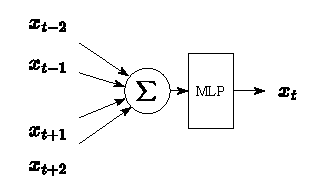
\includegraphics[width=\textwidth]{img/skipgram.pdf}
            \caption{Continuous Bag-of-Words}
            \label{fig:cbow}
        \end{subfigure}
        \hspace{-20px}
        \begin{subfigure}{0.45\textwidth}
            \centering
            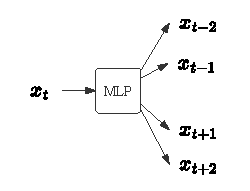
\includegraphics[width=0.75\textwidth]{img/cbow.pdf}
            \caption{Skip-gram}
            \label{fig:skipgram}
        \end{subfigure}
    \end{subfigure}
    \caption[Word2Vec objectives.]{The objectives employed by the Word2Vec algorithm \cite{mikolov2013distributed}. The algorithm here uses a context window of size $k=5$. In the (a) \emph{continuous bag-of-words} algorithm, we sum the embeddings of $k-1$ surrounding tokens and predict the original token. In the (b) \emph{skip-gram} algorithm, we use the original token for predicting the $k-1$ surrounding tokens.}
    \label{fig:word2vec}
\end{figure*}

The notion of using an embedding matrix for representing tokens is used also in neural \acp{lm} (\autoref{sec:lm-basics}). However, in majority of neural \acp{lm}, the embedding matrix is not trained separately with a specific algorithm, but s initialized randomly and trained jointly with the rest of the network via backpropagation.

\paragraph{Tokenization} For processing text as a sequence, we need to have a way of tokenizing the text, i.e. splitting it into discrete units. The most straightforward way would be to tokenize the text into either words or characters. Unfortunately, both of these approaches have major shortcomings. With word-level tokenization, we are not able to represent \emph{unknown} words, i.e., the words not seen in the training corpus. Word-level tokenization also considers morphologically similar words as independent units, forcing the model to learn their representation separately. Moreover, word-level tokenization becomes more difficult for languages such as Chinese, which do not separate words with spaces. In contrast, character-level tokenization uses a small and well-defined set of tokens, but the tokens are less meaningful and the resulting sequence is much longer, making the approach computationally inefficient. \cite[p.19]{jurafsky2024}

\emph{Subword tokenization}  is the middle ground between the word-level and character-level tokenization. It splits the text into smaller pieces called \emph{subwords}, which are continous character spans of various length. With subword tokenization, frequently used words typically get their own subword while less frequent words are split into multiple subwords. \cite[p.21]{jurafsky2024}

A subword tokenization algorithm that is commonly used in neural \acp{lm} is \emph{\acl{bpe}} (\acs{bpe}\glsunset{bpe}; \citealp{sennrich2016neural}). The \ac{bpe} algorithm starts with the vocabulary of individual bytes, iteratively merging the most frequent tokens and adding them to the vocabulary $V$ until we reach the target vocabulary size. An example subword tokenization of the expression ``Subword tokenization'' could be the subwords \texttt{ ['Sub', 'word', '▁token', 'ization']}, where ``\texttt{▁}'' is a special character denoting a preceding space.

There are also alternative sub-word tokenization algorithms, differing in their approach to constructing the vocabulary. WordPiece \cite{wu2016google} works similarly as BPE, but instead of the most frequent token choses the token which maximizes the likelihood of the training data. Unigram \cite{kudo2018subword} proceeds---unlike the previous algorithms---top-down, starting with a large vocabulary and progressively reducing the number of tokens to minimize unigram loss over the training data.


\subsection{Language Modeling}
\label{sec:lm-basics}
After introducing the main principles of neural networks and showing how to represent text in neural networks, we are ready to explain the notion of \emph{language modeling}, a central concept for building neural \acp{lm}.

\paragraph{Language Model} A \emph{language model} is a mathematical model that estimates a probability of a sequence of tokens $X = (x_1, \ldots, x_n)$. To estimate the probability, we can factorize the sequence probability using the chain rule:
\begin{align}
    P(X) = \prod_{i=1}^n P(x_i|x_1, \hdots, x_{i-1}).
\end{align}
This formulation gives us a way to compute the probability of the whole sequence as the product of probabilities of individual sequence prefixes.

\paragraph{\emph{n}-gram Language Model} An \emph{n}-gram \ac{lm} (parametrized by a positive integer $n$) further simplifies the product using the assumption that the probability of a token depends only on $n-1$ previous tokens \cite[p.32]{jurafsky2024}:
\begin{align}
    P(X) = \prod_{i=1}^T P(x_i|x_{i-n+1}, \hdots,x_{i-1}).
\end{align}

$n$-gram \acp{lm} store the counts of \emph{n}-gram occurrences over a training corpus in a look-up table. The probabilities are then estimated using these counts, interpolating over lower-order $n$-grams in case the specific $n$-gram did not occur in the training corpus. The main limitation of $n$-gram \acp{lm} (besides the size of the look-up tables) is the limit on the length of the context for each token, due to which \emph{n}-gram \acp{lm} fail to capture long-term dependencies \cite{bengio2000neural}.




\paragraph{Neural Language Model} A neural \ac{lm} is a \acl{lm} that estimates the text probability $P_\theta(X)$ using a neural network with parameters $\theta$. In contrast to \emph{n}-gram \acp{lm}, neural \acp{lm} can capture long-term dependencies and efficiently store the probability distribution in their parameters.

The parameters of the neural \ac{lm} are also estimated using a text corpus. For each word $x_i$ in the corpus, we aim to maximize the conditional probability that the model assigns to this word: $P_\theta(x_i|x_{<i})$ given preceding words in the context $x_{<i}$. If we express the gap between the model distribution $P_\theta$ and the empirical distribution of sequences in the corpus $P$ using cross-entropy, this formulation is equal to minimizing the negative log-likelihood of the next word \cite[p.158]{jurafsky2024}:
\begin{align}
    \mathcal{L}_{i} = - \log P_\theta(x_i|x_{<i}). \label{eq:clm}
\end{align}

This type of training is also called \emph{self-supervised}: each token naturally occurring in the corpus serves as the ground-truth label that the model aims to predict.


\subsection{Transformer Architecture}
\label{sec:transformer}
In this section, we pave the way towards the \emph{transformer} \cite{vaswani2017attention}: the core neural architecture used in \ac{nlp} nowadays. We describe its individual components and how the transformer is used for text processing.

\paragraph{Encoder-Decoder Framework}
We have described the \ac{rnn} (\autoref{sec:nns}) as a neural network that can \emph{encode} an input sequence into hidden states. The encoder-decoder framework \cite{sutskever2014sequence,cho2014learning}, originally introduced on top of \acp{rnn}, allows us to also \emph{generate an output sequence}. The idea is to use another network called the \emph{decoder} for generating the sequence, using the last hidden state of the encoder as its initial state. Here, we illustrate how the framework is applied using two \acp{rnn}:\footnote{We will later adapt the idea also for the transformer architecture.}

\begin{enumerate}
    \item The first \ac{rnn}, called the \emph{encoder}, encodes the sentence of input embeddings $\mathbf{X}= (\mathbf{x}_1, \ldots, \mathbf{x}_n)$ into a sequence of hidden states $\mathbf{H}_e = \{\mathbf{h}_e^{(0)}, \ldots, \mathbf{h}_e^{(n)}\}$ (where $\mathbf{h}_e^{(0)}$ is a null vector) by repeatedly applying a transformation $\mathcal{E}$ in each timestep $i\in(1,n)$:
          \begin{align}
              \mathbf{h}_e^{(i)} = \mathcal{E}(\mathbf{h}_e^{(i-1)}, \mathbf{x}_i).
          \end{align}
    \item The second \ac{rnn}, called the \emph{decoder}, uses $\mathbf{h}_e^{(n)}$ as its initial state $\mathbf{h}_d^{(0)}$ and produces the sequence of output tokens  $Y = (y_1, \ldots, y_m)$ by repeatedly applying a transformation $\mathcal{D}$ in each timestep $j\in(1,m)$:
          \begin{align}
              \mathbf{h}_d^{(j)}, y_j = \mathcal{D}(\mathbf{h}_d^{(j-1)}, y_{j-1}).
          \end{align}
\end{enumerate}

Note that the decoder produces the output sequence iteratively, yielding a token $y_j$ in each timestep, which is fed back as input in the next step. This process is called \emph{autoregressive decoding} and is described in more detail in \autoref{sec:plms}.

\paragraph{Attention Mechanism} We have mentioned that the hidden state of an \ac{rnn} used in every step has a fixed size, which limits the amount of information the network can capture about a sequence. The \emph{attention mechanism} \cite{bahdanau2015neural,luong-etal-2015-effective} bypasses this bottleneck by enabling the decoder to extract information dynamically from the whole encoded sequence.

At each step $j$, the decoder first computes a weight vector $\boldsymbol{\alpha}_j$: a probability distribution over the encoder hidden states. The coefficients $\alpha_{ji}$ are then used as weights in computing a context vector $\mathbf{c}_j$, which incorporates information from every hidden state of the encoder proportionally to its weight. The context vector is used as an additional input for the decoder:
\begin{align}
    \mathbf{h}_d^{(j)}, y_j = \mathcal{D}(\mathbf{h}_d^{(j-1)}, y_{j-1}, \mathbf{c}_j).
\end{align}


% At each step $j$, the decoder computes a context vector $c_j$ as the weighted sum of the hidden states of the encoder $\mathbf{H}_e$ using the attention matrix $\mathbf{W}_a$:
% \begin{align}
%   \alpha_{ji}  & = \operatorname{softmax}(\mathbf{h}_d^{(j)}\mathbf{W}_a \mathbf{h}_e^{(i)}), \\
%   \mathbf{c}_j & = \sum_i \alpha_{ji} \mathbf{h}_e^{(i)}.
% \end{align}




\paragraph{Transformer Architecture} The \emph{transformer}\footnote{Although \citet{vaswani2017attention} use ``Transformer'' with a capital ``T'', the orthography is gradually shifting towards the variant with a lowercase ``t''. See, e.g., \citet[p.~215]{jurafsky2024}.} \cite{vaswani2017attention} is a neural sequence processing architecture. Similarly as with \acp{rnn}, the input of the transformer is a sequence $\mathbf{X} \in \mathbb{R}^{n,d}$ and the output is the series of hidden states $\mathbf{H} \in \mathbb{R}^{n,d}$. Unlike \acp{rnn}, the transformer can process the sequence efficiently in parallel. To achieve that, the transformer replaces the \ac{rnn} hidden state---used previously as a mechanism for sharing information among tokens within a sequence---with the \emph{self-attention mechanism}.

Specifically, the transformer processes the input in a series of blocks. Each block is composed of two layers: (a) the \emph{self-attention layer} and (b) the \emph{\ac{mlp} layer}. The layers serve a different purpose: while the \ac{mlp} layer computes element-wise operations over each token, the self-attention layer enables sharing information among tokens.

\begin{itemize}
    \item \textbf{Self-attention layer}: Self-attention \cite{cheng2016long,vaswani2017attention} is a variant of the attention mechanism in which the source and the target states come from the same sequence. Given the input $\mathbf{X} \in \mathbb{R}^{n,d}$, the \emph{self-attention} produces the output $\mathbf{A} \in \mathbb{R}^{n,d}$ of the same size. For the state $\mathbf{x}_j \in \mathbf{X}$, the self-attention mechanism computes the vector $\mathbf{a}_j \in \mathbf{A}$ as a weighted combination of the value vectors $\mathbf{v}_i$ corresponding to the states $\mathbf{x}_i \in \mathbf{X}$:
          \begin{align}
              \mathbf{a}_j = \sum_{i\in 1..n} \alpha_{ji} \mathbf{v}_i,
          \end{align}
          where the \emph{value vector} $\mathbf{v}_i$ is computed using a trainable \emph{value matrix} $\mathbf{W_v} \in \mathbb{R}^{n,d}$:
          \begin{align}
              \mathbf{v}_i = \mathbf{x}_i \mathbf{W_v}.
          \end{align}
          To get the attention weights $\alpha_{ji}$, we first compute \textit{query} and \textit{key} vectors for each state using trainable matrices $\mathbf{W_q}$ and $\mathbf{W_k} \in \mathbb{R}^{n,d}$. Each weight is a normalized dot product of the corresponding vectors:
          \begin{align}
              \mathbf{q}_i & = \mathbf{x}_i \mathbf{W_q},                                                     \\
              \mathbf{k}_i & = \mathbf{x}_i \mathbf{W_k},                                                     \\
              \alpha_{ji}  & = \operatorname{softmax}\biggl(\frac{\mathbf{q}_j\mathbf{k}_i}{\sqrt{d}}\biggr),
          \end{align}
          where $\operatorname{softmax}(\mathbf{x}) = \frac{\exp(\mathbf{x})}{\sum_i \exp(\mathbf{x}_i)}$. The operations can be efficiently parallelized using matrix multiplication:
          \begin{align}
              \mathbf{Q}                                             = \mathbf{X}\mathbf{W_q},\quad\mathbf{K} & = \mathbf{X}\mathbf{W_k},\quad\mathbf{V} = \mathbf{X}\mathbf{W_v},                          \\
              \operatorname{attn}(\mathbf{Q}, \mathbf{K}, \mathbf{V})                                         & = \operatorname{softmax}\biggl(\frac{\mathbf{Q}\mathbf{K}^\top}{\sqrt{d}}\biggr)\mathbf{V}.
          \end{align}
          To capture different aspects of the input sequence, transformer uses $k$ \emph{attention heads}. Each head $\mathcal{H}_i$ is parametrized by a set of attention matrices $\mathbf{W}^{(\mathcal{H}_i)}_\mathbf{q}$,$\mathbf{W}^{(\mathcal{H}_i)}_\mathbf{k}$, and $\mathbf{W}^{(\mathcal{H}_i)}_\mathbf{v}$, computing the self-attention as described above. To compute the output of the self-attention layer, the output of each head is concatenated and linearly transformed using the trainable output matrix $\mathbf{W}_o$:
          \begin{align}
              \mathbf{A} = \operatorname{concat}(\operatorname{attn}^{(\mathcal{H}_1)}, \ldots, \operatorname{attn}^{(\mathcal{H}_k)})\mathbf{W}_o.
          \end{align}
    \item \textbf{\ac{mlp} layer:} The \ac{mlp} layer processes the outputs of the self-attention layer with a two-layer \ac{mlp}. Specifically, it applies two linear transformations with a non-linear activation function $f$ in between:
          \begin{align}
              \mathbf{H} = f(\mathbf{a}_j\mathbf{W}_1 + \mathbf{b}_1)\mathbf{W}_2 + \mathbf{b}_2,
          \end{align}
          where $\mathbf{W}_1 \in \mathbb{R}^{d,d_{\text{ff}}}$, $\mathbf{W}_2 \in \mathbb{R}^{d_{\text{ff}},d}$, $\mathbf{b}_1 \in \mathbb{R}^{d_{\text{ff}}}$, and $\mathbf{b}_2 \in \mathbb{R}^{d}$ are the trainable parameters and $d_{\text{ff}}$ is the dimensionality of the hidden layer. Note that the operations in the \ac{mlp} layer are element-wise (applied separately to each $\mathbf{a}_j$), so the transformation can be computed efficiently in parallel.
\end{itemize}
To stabilize the training process, the input of each layer (or output, depending on the architecture variant) is normalized using \emph{layer normalization} \cite{ba2016layer}. Another feature that helps to stabilize training is the \emph{residual connection}: the fact that the output of the $i$-th layer is summed with its original input $\mathbf{H}^{(i)}$:
\begin{align}
    \mathbf{H}^{(i+1)} = \mathbf{H}^{(i)} + \operatorname{layer}(\mathbf{H}^{(i)}).
\end{align}
This way, the model can learn to adjust the input representation rather than completely replacing it.

To get the input representation $\mathbf{H}^{(0)}$, we sum the token embeddings $\mathbf{X} \in \mathbb{R}^{n,d}$ with \emph{positional embeddings}. Positional embeddings encode the absolute or relative position information of individual tokens, which would otherwise get lost in parellized processing.\footnote{There are multiple variants of positional embeddings with various trade-offs; see \citet{dufter2022position} for an overview.}



\begin{figure*}[ht]
    \centering
    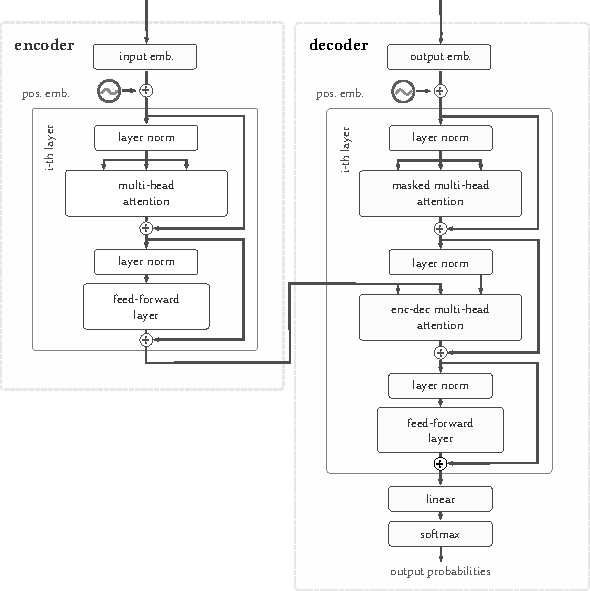
\includegraphics[width=0.9\textwidth]{img/transformer.pdf}
    \caption[The transformer architecture.]{An encoder-decoder variant of the transformer architecture. The encoder has $N_{e}$ blocks, each consisting of a \emph{self-attention} and \emph{MLP layer}. The decoder has $N_{d}$ blocks with \emph{masked self-attention} and \emph{encoder-decoder attention}, again followed by an \emph{MLP layer}. The input to each layer is normalized using \emph{layer norm}. After the last decoder block, the output probabilities are computed using a linear projection and softmax. The figure is adapted from \href{https://github.com/bbycroft/llm-viz/blob/main/src/llm/intro-image.svg}{https://github.com/bbycroft/llm-viz}.}
    \label{fig:transformer}
\end{figure*}



% We train the model on \emph{batches} of data, using an optimization algorithm such as \acl{sgd} (\acs{sgd}\glsunset{sgd}; \citealp[p.~275]{goodfellow2016deep}) or Adam \cite{kingma2014adam}. The batch size $b$ and the learning rate $\alpha$ are the training hyperparameters.
As shown in \autoref{fig:transformer}, which summarizes the architecture details discussed so far, the original transformer architecture is based on the encoder-decoder framework. The decoder blocks implement two additional features:
\begin{itemize}
    \item Each block contains an additional layer called the \emph{encoder-decoder attention}. In contrast to the self-attention mechanism, the \emph{keys} and \emph{values} come from the last block of the encoder, enabling the decoder to attend to the encoded sequence.
    \item The self-attention is \emph{masked} so that each token can collect information only from the preceding tokens, which is necessary to enable training the model for left-to-right autoregressive decoding.
\end{itemize}

The hidden states produced by the transformer can be used for language modeling: after the last decoder block, the hidden states are projected into a matrix of size $\mathbb{R}^{|V|\times n}$ and normalized using softmax, producing a probability distribution over the vocabulary for each input token.

\paragraph{Text Generation} For generating text from a transformer decoder, we can use \textit{left-to-right autoregressive decoding} \cite[p.196]{jurafsky2024}. The decoding process starts by feeding a special \texttt{<s>} (beginning of sequence) token into the decoder and iteratively selecting the \emph{i}-th token based on the model-predicted probability distribution for the \emph{i}-th position. The decoding stops once a special \texttt{</s>} (end of sequence) token is decoded. The procedure is outlined in Algorithm \ref{alg:decoding}.
\begin{algorithm}[ht]
    \begin{algorithmic}[1]
        \State{Initialize: $Y= \texttt{<s>}, y = \texttt{<s>}$ \Comment{Output sequence, current token}}
        \While{$y \neq \texttt{</s>}$}
        \State Predict next token probability distribution: $p(y | Y)$
        \State Select the next token: $y \sim p(y | Y)$ \label{alg:dec:sample}
        \State Update output sequence: $Y = Y \cup y$
        \EndWhile
        \State Return $Y$
    \end{algorithmic}
    \caption{Autoregressive decoding}
    \label{alg:decoding}
\end{algorithm}

\noindent The token selection step (line \ref{alg:dec:sample}) can be realized in various ways, including:
\begin{itemize}
    \item \textbf{Greedy decoding}: Selecting the most probable token: $y_i = \argmax{y \in V} p_\theta(y|y_{<i}).$
    \item \textbf{Beam search}: Extending the $k$ most probable sequences from the previous step with the next tokens, and selecting the $k$ most probable sequences for the next step.
    \item \textbf{Top-$k$ sampling}: Sampling the next token from the distribution of $k$ most probable tokens.
    \item \textbf{Top-$p$ (nucleus) sampling} \cite{holtzman2019curious}: Sampling the next token from the distribution of tokens with cumulative probability $p$.
\end{itemize}
While greedy decoding and beam search are used to generate more probable sequences (approximating the exact algorithm for estimating the most probable sequence overall, which has exponential complexity), sampling algorithms are used to decode more creative outputs. Notet that the list of the decoding algorithms as presented here is not exhaustive; see \citet{zarriess2021decoding} and \citet{wiher2022decoding} for an overview and further discussion.

\subsection{Pretrained Language Models}
\label{sec:plms}
To achieve good performance on an \ac{nlp} task with a vanilla transformer model, we need an extensive amount of labeled training data. A more efficient workflow is as follows: the models are first \emph{pretrained} on large-scale data---such as The Pile \cite{gao2020pile}, or C4 \cite{raffelExploringLimitsTransfer2019}---and then \emph{finetuned} for downstream tasks on a smaller, task-specific dataset. Crucially, the pretraining is \emph{self-supervised} (cf. \autoref{sec:lm-basics}), i.e., it can be done using general domain-data with no specific annotations. Although pretraining a model still requires significant computational resources, the checkpoints of \acp{plm} can be used for efficient finetuning on downstream tasks.


\begin{table}[t]
    \footnotesize
    \centering
    \begin{tabular}{lllp{4.5cm}}
        \toprule
        \textbf{Type}            & \textbf{Example Models}                              & \textbf{\# Parameters}  & \textbf{Note}                                            \\
        \midrule
        \multirow{3}{*}{Encoder} & BERT \cite{devlinBERTPretrainingDeep2019}            & 110M-340M               & landmark pretrained encoder                              \\
                                 & RoBERTa \cite{liuRoBERTaRobustlyOptimized2019}       & 125M-355M               & improves BERT pretraining                                \\
                                 & \textsc{LaserTagger} \cite{malmi2019lasertagger}     & 110M                    & text-editing model                                       \\
        \midrule
        \multirow{3}{*}{Enc-Dec} & BART \cite{lewisBARTDenoisingSequencetoSequence2019} & 139M-406M               & \multirow{2}{*}{landmark encoder-decoders}               \\
                                 & T5 \cite{raffelExploringLimitsTransfer2019}          & 220M-11B                &                                                          \\
                                 & mBART \cite{liuMultilingualDenoisingPretraining2020} & 680M                    & multilingual version of BART                             \\
        \midrule
        \multirow{3}{*}{Decoder} & GPT-2 \cite{radfordLanguageModelsAre2019}            & 117M-1.5B               & landmark pretrained decoder                              \\
                                 & Llama2 \cite{touvronLlamaOpenFoundation2023}         & \multirow{3}{*}{7B-70B} & \multirow{3}{*}{large language models (§\ref{sec:llms})} \\
                                 & Mistral \cite{jiangMistral7B2023}                    &                         &                                                          \\
                                 & Zephyr \cite{tunstallZephyrDirectDistillation2023}   &                         &                                                          \\
        \bottomrule
    \end{tabular}
    \caption[Transformer architectures and models.]{Types of transformer architectures and specific models used in this work. The number of parameters may vary based on the model variant.}
    \label{tab:pretrained_models}
\end{table}


\paragraph{Model types} Depending on the downstream task, different variants of the transformer architecture are used:

\begin{itemize}
    \item \textbf{Encoder models} \cite{devlinBERTPretrainingDeep2019,liuRoBERTaRobustlyOptimized2019} use only the \emph{encoder} part of the transformer architecture. These models are not generative; instead, they produce a contextualized representation of the input sequence $\mathbf{X}$. The representation can be used for downstream tasks such as sequence classification, sequence tagging, or computing sequence similarity.
    \item \textbf{Encoder-decoder models} \cite{lewisBARTDenoisingSequencetoSequence2019,raffelExploringLimitsTransfer2019} use the original \emph{encoder-decoder} architecture, and are explicitly trained to transform an input sequence $\mathbf{X}$ into a target sequence $\mathbf{Y}$. Encoder-decoder models are mostly used for sequence-to-sequence tasks, such as \ac{mt}, question answering, or summarization.
    \item \textbf{Decoder models} \cite{radford2018improving,radford2019language} use only the \emph{decoder} part of the transformer architecture, which makes them suitable for generating text continuations. While seemingly less expressive, the models can be used for the same tasks as the encoder-decoder models, using the input sequence $\mathbf{X}$ as the prefix for  generating the output sequence $\mathbf{Y}$.
\end{itemize}

\autoref{tab:pretrained_models} shows examples of the \acp{plm} for each category, focusing on the models relevant for this work.


\paragraph{Pretraining objectives} There are multiple ways to use the ground truth sequence for pretraining the transformer models (see \autoref{fig:objectives} for illustration):


\begin{itemize}
    \item \textbf{Masked Language Modeling}: The goal is to predict a token at a masked position given both its left and right context. This objective is inspired by the Cloze task in psychology, where a similar task is given to human subjects \cite{taylor1953cloze}. The objective is commonly used for encoder-only models such as BERT \cite{devlinBERTPretrainingDeep2019}.
    \item \textbf{Text Denoising}: The goal is generally to predict the original sequence from its corrupted version. This objective combines masked language modeling with other tasks such as predicting a deleted token or predicting a number of missing tokens. It is used for pretraining encoder-decoder models such as BART \cite{lewisBARTDenoisingSequencetoSequence2019} or T5 \cite{raffelExploringLimitsTransfer2019}.
    \item \textbf{Causal language modeling}: The goal is to predict the next token given the previous sequence of tokens, as described in \autoref{eq:clm}. This objective is used for pretraining decoder-only models, including GPT-2 \cite{radford2019language} and most of \acp{llm}.
\end{itemize}

As a matter of fact, only causal language modeling adheres to the strict definition of a language model as given in \autoref{sec:lm-basics} \cite{cotterell2024formal}. However, all of these objectives are used in practice and are often combined with other auxiliary objectives such as next sentence prediction or token frequency prediction \cite{aroca2020losses}.

\begin{figure*}[t]
    \centering
    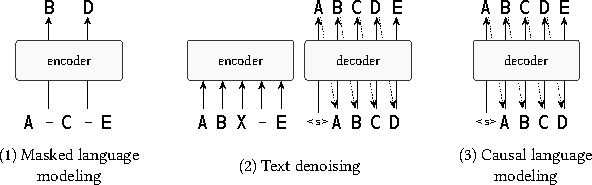
\includegraphics[width=0.9\textwidth]{img/objectives.pdf}
    \caption[Pretraining objectives.]{A scheme of the common objectives used by pretrained models: (1) masked language modeling, (2) text denoising, (3)  causal language modeling. The special symbol \texttt{<s>} (beginning of a sentence) is used to bootstrap the decoding process.}\label{fig:objectives}
\end{figure*}


\paragraph{Finetuning} By \emph{finetuning} a model, we mean additional training of a pretrained model on a task-specific dataset. Finetuning a pretrained model is more efficient than training a model from scratch, as the pretrained representations provide a warm start for the training process. However, finetuning typically cannot be applied repeatedly on the same model: repeated model updates can lead to erasing previous knowledge, also known as \emph{catastrophic forgetting} \cite{mccloskey1989catastrophic,kirkpatrick2017overcoming}.\footnote{This problem is partially mitigated by multi-task finetuning, in which the tasks are unified under a pre-specified input format and the model is finetuned for all the tasks at once \cite{sanh2021multitask,xieUnifiedSKGUnifyingMultiTasking2022}.}


\paragraph{Few-shot and Zero-shot Settings} If the size of the finetuning data is very limited (up to a few hundred examples), we talk about \emph{few-shot} setting. By limiting the finetuning data to zero, we arrive at a \emph{zero-shot} setting, where we use a model on a task which it has not been trained for. These settings are crucial for tasks with scarce data, also called \emph{low-resource scenarios}. \cite{hedderich2021survey}


\subsection{Large Language Models}
\label{sec:llms}
Scaling the models in terms of the number of parameters and the size of the training data has turned out to further improve the performance of the models \cite{kaplan2020scaling,hoffmann2022training}. Larger models were shown to exhibit unprecedented capabilities in terms of language fluency, language understanding, and reasoning skills \cite{wei2022emergent,bubeck2023sparks}, giving name to a specific category of \emph{\aclp{llm} (\acsp{llm}\glsunset{llm};} \citealp{brown2020language,zhao2023survey}). Broadly speaking, \acp{llm} are transformer decoders with billions of parameters \cite{yang2024harnessing}.

At the time of writing, \acp{llm} are becoming an omnipresent phenomenon in most of \ac{nlp} areas. In many \ac{nlp} tasks, from document-level translation \cite{wang2023documentlevel} and \ac{mt} evaluation \cite{kocmiLargeLanguageModels2023} to news summarization \cite{zhang2024benchmarking} and story generation \cite{xie2023next}, \acp{llm} have comparable or better performance than previous task-specific approaches.

Although the most performant \acp{llm} are currently available only through proprietary APIs \cite{chatgpt,openai2023gpt4,team2023gemini,anthropic2024claude}, there is an increasing amount of performant open-access \acp{llm} \cite{jiangMistral7B2023,touvronLlamaOpenFoundation2023} available through platforms such as HuggingFace Transformers \cite{wolf2019HuggingFacesTS}.

\paragraph{In-context Learning} \acp{llm} can perform certain tasks without the need for finetuning on task-specific data $E_{\text{task}} = \{(x_1, y_1), \ldots, (x_n, y_n)\}$. Instead of training, we provide $E_{\text{task}}$ as a part of the \emph{prompt} (i.e., the text used as a decoding prefix). After $E_{\text{task}}$, we also append our test input $x_{n+1}$. By the virtue of causal language modeling and using other examples for the context, the model can be expected to decode the corresponding output $\hat{y}_{n+1}$. This ability is known as \emph{in-context learning} \cite{brown2020language,dong2022survey}. As the set of input-output examples is usually limited by the context size, we talk about \emph{few-shot prompting}.

\paragraph{Instruction Tuning} Another key to strong cross-task performance of \acp{llm} is instruction tuning: finetuning on a large dataset of tasks formulated using natural language instructions, such as \textit{``Answer this question: \{question\}''} or \textit{``Translate this sentence: \{sentence\}''} \cite{sanh2021multitask,ouyang2022TrainingLM}. Due to their strong generalization abilities, the instruction-tuned models can be prompted to perform a task of choice in natural language, even without being directly trained for it. This allows to use the model for the task with no examples in the context, a setting known as \emph{zero-shot prompting}.



\section{Data-to-Text Generation}
\label{sec:d2t}
In this section, we provide background for the task of \acl{d2t} generation. First, we present the task itself along with its applications (\autoref{sec:d2t-tasks}) and the subtasks to which \ac{d2t} generation can be decomposed (\autoref{sec:d2t-pipeline}). For the subtasks, we present rule-based (\autoref{sec:rule-d2t}), statistical (\autoref{sec:stat-d2t}), and neural (\autoref{sec:neural-d2t}) approaches. In the final part, we describe the \ac{d2t} datasets (\autoref{sec:datasets}) and evaluation metrics (\autoref{sec:evaluation}) we use in the thesis.

\subsection{Task and Applications}
\label{sec:d2t-tasks}

\ac{d2t} generation is an umbrella term for tasks that require transforming structured data into natural language. The input can take various forms, including graphs, trees, 2D tables, charts, or databases. The output is a fluent text that accurately conveys the information from the data \cite{gattSurveyStateArt2018,sharmaInnovationsNeuralDatatotext2022}.

Before we talk about \ac{d2t} generation from the research point of view, we present an overview of its practical applications:

\begin{itemize}
    \item \textbf{Automated Journalism}: Augmenting (or, in simple cases, even replacing) human journalists for writing data-based reports, including:
          \begin{itemize}
              \item \textbf{News reports}: Automating news writing, e.g., for election results \cite{leppanen2017data}, incidents \cite{vanderleeCACAPODatasetMultilingual2020}, earthquakes \cite{oremus2014first}, or wildlife tracking \cite{siddharthan2012blogging,ponnamperuma2013tag2blog}.
              \item \textbf{Sport reports}: Generating game summaries for sports such as basketball \cite{wiseman2017challenges,thomson2020sportsett}, baseball \cite{puduppullyDatatotextGenerationEntity2019}, or soccer \cite{van2017pass}.
              \item \textbf{Financial reports}: Supporting financial decisions by generating comments on stock prices \cite{murakami2017learning,aoki2018generating} and summarizing financial documents \cite{chapman2022towards}.
              \item \textbf{Weather reports}: Generating weather forecasts and weather-related reports \cite{goldberg1994using,belz2005corpus,belz2008automatic,angeli-etal-2010-simple,balakrishnan2019constrained}.
          \end{itemize}
    \item \textbf{Business Intelligence Reports}: Providing decision support in business reports alongside data summaries and visualizations (mostly developed by commercial companies such as Arria\footnote{\url{https://www.arria.com}}, InfoSentience\footnote{\url{https://infosentience.com}}, or vPhrase\footnote{\url{https://www.vphrase.com}}; see also \citet{daleNavigatingTextGeneration2023} for a recent overview).
    \item \textbf{Chart Captioning}: Generating captions\footnote{In contrast to image captioning \cite{stefanini2022show}, here the systems can rely on the underlying data in textual form (although the approaches can be hybrid, see e.g. \citealp{kantharajCharttoTextLargeScaleBenchmark2022}).} for charts or graphs, e.g., for assistive technologies, document indexing, or simplifying decision support \cite{demirGeneratingTextualSummaries2008,demirSummarizingInformationGraphics2012,obeidCharttoTextGeneratingNatural2020,kantharajCharttoTextLargeScaleBenchmark2022}.
    \item \textbf{Healthcare Summaries}: Providing clinical data summaries about patients to clinicians \cite{portet2009automatic,scott2013data}, or providing medical information to patients, e.g., for behavioral change \cite{reiter2003lessons} or nutritional counseling \cite{balloccu-reiter-2022-comparing}.
    \item \textbf{Product Descriptions}: Automating generating product descriptions in specific domains such as for laptops and TVs \cite{wen2015toward,wen2016multi}, or general-domain approaches for big e-commerce platforms \cite{shaoControllableDiverseText2021,kotoCanPretrainedLanguage2022}.
\end{itemize}

\subsection{D2T Generation Pipeline}
\label{sec:d2t-pipeline}


Until recently, \ac{d2t} generation was decomposed into approximately 4-6 subtasks\footnote{The count is only approximate: for example, \citet{milleModD2TMultilayerDataset2023} further subdivides some of the subtasks, leading to 10 subtasks in total.} which were addressed separately \cite{reiterBuildingAppliedNatural1997,Reiter_Dale_2000,reiterArchitectureDatatoTextSystems2007,gattSurveyStateArt2018}. Even though recent advances enable approaches which solve the task in an \emph{end-to-end} fashion (i.e., without intermediate steps), the subtasks are still relevant for conceptualization of \ac{d2t} generation. We choose to split the pipeline into five representative subtasks, as illustrated in \autoref{fig:pipeline}:

\begin{enumerate}
    \item \textbf{Content Selection}: Deciding which facts from the structured data
          to include in the text.
    \item \textbf{Document Planning}: Determining the order of the
          facts and dividing the facts into paragraphs.
    \item \textbf{Sentence Planning}: Aggregating the facts into
          sentences.
    \item \textbf{Lexicalisation}: Transforming the facts to text segments.
    \item \textbf{Surface Realisation}: Combining the text segments into a well-formed text in natural language.
\end{enumerate}


\begin{figure*}[t]
    \centering
    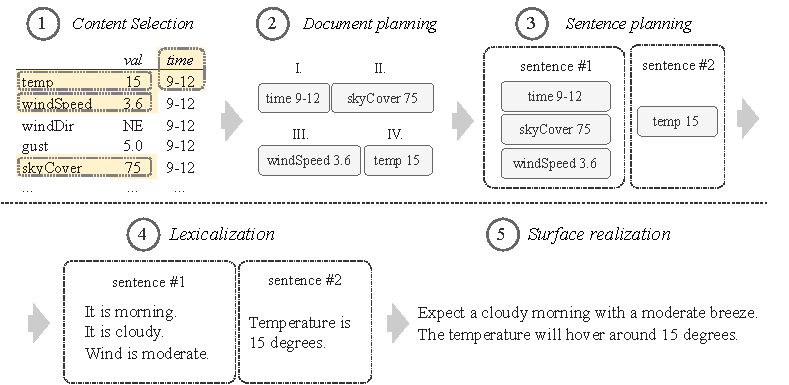
\includegraphics[width=\textwidth]{img/pipeline.pdf}

    \caption[A data-to-text generation pipeline.]{A five-step \ac{d2t} generation pipeline on the example of generating a weather forecast. (1) The relevant fields for the forecast are selected from the data table. (2) The fields are ordered. (3) The ordered fields are aggregated into sentences. (4) Each field is transformed into a text segment. (5) The text segments are combined into the final text.}\label{fig:pipeline}

\end{figure*}


Decomposing \ac{d2t} generation into subtasks helps to modularize the system. Each module has a specific and well-defined function, which makes the system more explainable. Modularization also enables realizing each subtask using a different approach (see \Cref{sec:rule-d2t,sec:stat-d2t,sec:neural-d2t}).

The subtasks are typically executed in a \emph{pipeline}, i.e., the input is sequentially processed by a series of modules. The main issue of pipeline-based approaches is error accumulation: the errors from one module propagate to downstream modules. Despite this issue, the pipeline approach is the basis of many rule-based \ac{d2t} generation systems \cite{milleModD2TMultilayerDataset2023} and can also benefit neural-based systems (\citealp{moryossef2019step,puduppullyDatatotextGenerationMacro2021}; see also \autoref{sec:pipeline}).


\subsection{Rule-based Approaches}
\label{sec:rule-d2t}

By \emph{rule-based approaches} for \ac{d2t} generation, we mean the approaches using manually defined rules or grammars.\footnote{In contrast to the data-driven approaches (presented in \Cref{sec:stat-d2t,sec:neural-d2t}), which derive the system's inner workings from the data.} Rule-based approaches are still in use in various forms today \cite{gattSurveyStateArt2018,daleNaturalLanguageGeneration2020,daleNavigatingTextGeneration2023}. It is helpful to view these approaches through the lens of the whole \ac{d2t} generation pipeline (\autoref{sec:d2t-pipeline}), as these approaches typically tackle particular subtasks of the pipeline individually.


\paragraph{Content Selection}
Extracting meaningful information from the data typically relies on domain-specific heuristics, e.g., \textit{``if a pattern is detected in the signal, include it in the report''} \cite{portet2009automatic}. Various factors can influence the decision, including the target length of the report, the type of the report, and its target audience \cite{gkatziaContentSelectionDatatoText2016}.

\paragraph{Text Planning} Rule-based text planning follows discourse strategies which are designed to satisfy the desired communicative goals (such as \emph{define}, \emph{compare}, or \emph{describe}; \citealp{mckeown1985text}). The resulting rules are typically in the form \textit{``if a player scores two consecutive goals, describe these in the same sentence''}  \cite{gattSurveyStateArt2018}.


\paragraph{Template-based Lexicalization \& Surface Realization}
Simpler rule-based approaches for lexicalization and surface realization are typically based on \emph{templates}: pre-written text snippets with placeholders which are filled with values from the data. Templates can range from simple fill-in-the-blank approaches (such as \textit{``The temperature will be \{temp\} degrees''}) to more sophisticated templates using a templating language \cite{gatt2009simplenlg,reiter2016nlg}.  Rules are used for selecting the templates, combining them, and filling the placeholders with values (with the last step being non-trivial in languages with rich morphology \cite{duvsek2019neural}). The resulting rule-based system is usually tied to a specific task and domain, but it can be a way to generate outputs of sufficient quality with reasonable development time and costs \cite{vanderleeAutomatedLearningTemplates2018}.


\paragraph{Grammar-based Lexicalization \& Surface Realization}
A different way to handle lexicalization and surface realization in rule-based systems is using grammar-based approaches. Even though a \emph{grammar} is technically also a set of rules, it differs by the fact that it describes the production rules for the whole sentence.
Grammar-based approaches are rooted in linguistic theories, such as systemic grammars \cite{halliday1985systemic,matthiessen1991lexico} or meaning-text theory \cite{mel1988dependency,goldberg1994using}. The implementation typically relies on off-the-shelf realizers such as FUF/SURGE \cite{elhadad1997surge} or KPML \cite{bateman1997enabling}. Grammar-based approaches are more general-purpose than rule-based approaches; however, they require considerable manual effort, detailed input, and often also additional rules for choosing among multiple valid outputs \cite{gattSurveyStateArt2018}.
% FORGe \cite{milleFORGeWebNLG20172017,mille2019teaching}


\subsection{Statistical Approaches}
\label{sec:stat-d2t}
The idea of statistical\footnote{Since statistical \ac{d2t} generation approaches overlap with classical machine learning methods, these approaches are perhaps better described as \emph{pre-neural data-driven} approaches. However, we will stick to the more established term.} \ac{d2t} generation approaches is to derive some part of a \ac{d2t} generation system from statistics of a text corpus. This may apply both to individual steps of the \ac{d2t} generation pipeline (estimating parameters of a specific module) or for parametrizing an end-to-end system \cite{liang2009learning,dusekTrainingNaturalLanguage2015}. This idea is not mutually exclusive with rule-based and grammar-based approaches; in fact, corpus statistics were initially used for re-ranking the outputs generated from a grammar-based system \cite{bangalore2000corpus,langkilde2000forest,ratnaparkhi2000trainable} or even integrated directly at the level of generation decisions \cite{belz2008automatic}.

Even fully data-driven approaches still relied on grammatical rules; the only difference was that these rules were derived from treebanks, i.e., text corpora annotated with syntactic and semantic sentence structures. For example, the approach of \citet{white2007towards} relied on a Combinatory Categorial Grammar \cite{steedman2001syntactic} derived from the Penn Treebank \cite{hockenmaier2007ccgbank}. Hybrid approaches combined a set of hand-written rules or grammars with statistical models \cite{konstas2012concept,gardent2017statistical}.

The earlier stages of the \ac{d2t} generation pipeline, such as content selection or text planning, were usually tackled by \emph{unsupervised} machine learning methods. For example, \citet{duboue2003statistical} proposed to use a clustering-based method for content selection, estimating the relative importance of each cluster for the final text. \citet{barzilay2004catching} modelled the content structure using Hidden Markov Models \cite{baum1966statistical}, learning the structure from unannotated documents. An example of a statistical approach for text planning is presented in \citet{liang2009learning}, who learn latent alignment between the text and the data for text segmentation and structuring.

\subsection{Neural Approaches}
\label{sec:neural-d2t}
Building upon the previous data-driven approaches, neural networks (see \autoref{sec:nns}) began to be studied more widely in the context of \ac{d2t} generation around 2015 \cite{wen2015toward,dusekSequencetoSequenceGenerationSpoken2016}. Thanks to advances in hardware \cite{hooker2021hardware} and efficient learning from large data \cite{lecun2015deep}, neural networks enabled not only building more powerful modules for the \ac{d2t} generation pipeline but also replacing the pipeline entirely with end-to-end models \cite{dusekEvaluatingStateoftheartEndtoEnd2020}. For a more detailed overview of neural \ac{d2t} generation in recent years, we point the reader to the surveys of \citet{sharmaInnovationsNeuralDatatotext2022} and \citet{lin2023survey}; here, we mainly focus on the concepts and model architectures related to this thesis.


\paragraph{Linearization} To get an input sequence suitable for the neural model, structured data first needs to be converted into a sequence of tokens. To preserve the data structure while keeping the input simple, a common practice is to \emph{linearize} the input: convert the data to a minimalistic representation with a handful of dedicated special tokens serving as delimiters. An example linearization of a knowledge graph is depicted in \autoref{fig:linearization}~(c). Linearization can be very effective \cite{yang2020improving,hoyle2021promoting,xieUnifiedSKGUnifyingMultiTasking2022}, beating specialized representations such as graph embeddings \cite{marcheggianiDeepGraphConvolutional2018,koncel-kedziorskiTextGenerationKnowledge2019}.

\begin{figure*}[h]
    \centering
    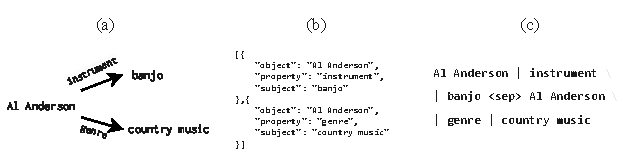
\includegraphics[width=\textwidth]{img/linearization.pdf}

    \caption[Knowledge graph representations.]{Representations of a simple knowledge graph: (a) the original knowledge graph, (b) JSON representation, (c) linearized representation.}\label{fig:linearization}

\end{figure*}

% Along with linearization, we can also use special embeddings for the structural elements (e.g., for table rows and columns), which are summed with the positional and token embeddings \cite{wang2021tuta,yangTableFormerRobustTransformer2022}. Since these additional embeddings need to be learned, this approach is more suitable for high-resource tasks.

\paragraph{Delexicalization} A specific data value may appear only a few or zero times in the training data, making it difficult for the model to learn its representation. Delexicalization is the process of replacing the values with placeholders, allowing the model to work only with the fill-in-the-blank templates instead of actual values \cite{oh2000stochastic,mairesse2010phrase,wen2015semantically,dusekSequencetoSequenceGenerationSpoken2016}. The values are filled in the post-processing step using simple rules, akin to template-based systems. This approach was shown to be useful even for languages with rich morphology, where the values can be inflected using a dedicated language model \cite{duvsek2019neural}.

\paragraph{Sequence-to-Sequence Generation} Generating text from data in the end-to-end fashion, i.e., without intermediate steps, is enabled by neural \ac{seq2seq} models. \Ac{seq2seq} models are designed for transforming variable-length input sequences into variable-length output sequences \cite{cho2014learning,sutskever2014sequence}. The typical \ac{seq2seq} architecture is the encoder-decoder framework described in \autoref{sec:transformer}. In the case of \ac{d2t} generation, the input sequence is the linearized version of structured data, and the output sequence is the target text.

\paragraph{RNN-based Approaches} The original seq2seq approaches were designed for \ac{mt} \cite{cho2014learning,sutskever2014sequence}, but soon were also adopted for other \ac{nlg} tasks.  \citet{wen2015semantically} and \citet{dusekSequencetoSequenceGenerationSpoken2016} adopted \acp{rnn} for generating the response in a dialogue system, using a structured representation of the dialogue act as the input. \citet{mei2016talk} use \acp{rnn} to address also the content selection step, identifying salient data records using the attention mechanism for generating weather reports.

An important addition to \ac{rnn}-based approaches was the \emph{copy mechanism}, which allows the model to generate the tokens by copying them from the input sequence \cite{gu2016incorporating,seeGetPointSummarization2017}. The copy mechanism is an alternative to delexicalization, enabling the model to fill in lexical values by itself. Unlike delexicalization, the copy mechanism is trainable along with the rest of the model \cite{gehrmannEndtoEndContentPlan2018}.

\acp{rnn} were still used even after the introduction of the transformer model (\autoref{sec:transformer}), since they tend to work better in low-resource settings. For example, \citet{freitagUnsupervisedNaturalLanguage2018} experimented with using a text denoising objective to pretrain an \ac{rnn}-based system for \ac{d2t} generation. For adapting an \ac{rnn}-based model to other domains, \citet{wen2020recurrent} proposed \emph{data counterfeiting}, i.e., replacing delexicalized slots with slots from another domain. To improve the faithfulness of the outputs, \citet{rebuffel2021controlling} propose an architecture based on three \acp{rnn} focusing separately on content, faithfulness, and fluency. Various shared tasks and comparisons \cite{gardentWebNLGChallengeGenerating2017,dusekEvaluatingStateoftheartEndtoEnd2020,ferreiraNeuralDatatotextGeneration2019} showed that RNN-based approaches were generally competitive with rule-based approaches: the RNNs produce more fluent text, while the pipeline-based approaches make less semantic errors.


\paragraph{PLM-based Approaches} Using a transformer model for \ac{d2t} generation became practical with the arrival of \acp{plm} discussed in \autoref{sec:plms}. As an example, the 2020 WebNLG+ shared task (see \autoref{sec:datasets}) was dominated by systems based on pretrained encoder-decoder transformer models (\citealp{ferreira20202020}).

\acp{plm} made it possible to remove both \emph{delexicalization} and \emph{copy mechanism}. The general language modeling pretraining, along with the learned ability to copy tokens from the input, allow the model to handle rare entities not present in the task-specific training data. \acp{plm} are also able to produce outputs with considerably better fluency than \ac{rnn}-based models. Moreover, variants of \acp{plm} pretrained on multilingual corpora \cite{liuMultilingualDenoisingPretraining2020,xueMT5MassivelyMultilingual2021} are able to produce outputs in a variety of languages.

Due to the advantages above, \ac{plm}-based approaches excel in low-resource settings, which are common for many \ac{d2t} generation tasks. Following \citet{chenFewShotNLGPreTrained2019}, other works adopted PLMs for few-shot or zero-shot \ac{d2t} generation. In these scenarios, the models are typically finetuned on domain-specific data for few-shot generation \cite{changNeuralDatatoTextGeneration2021,suFewShotTabletoTextGeneration2021} or on related domains for zero-shot generation (see \autoref{sec:pipeline}). Improving \ac{plm}-based \ac{d2t} generation in English revolves mainly around (1) finding \emph{suitable data representations} and (2) ensuring the \emph{semantic accuracy} of the outputs, both of which we will discuss in the following chapters.

\paragraph{LLM-based Approaches} At the time of writing, approaches using \acp{llm} for \ac{d2t} generation are still in naissance. Works which compared zero-shot or few-shot \ac{llm} prompting with finetuned \acp{plm} on existing datasets have found that \acp{llm} rank behind state-of-the-art finetuned models on automatic metrics \cite{axelssonUsingLargeLanguage2023,yuanEvaluatingGenerativeModels2023}. In \autoref{sec:quintd}, we will also show that \acp{llm} can be employed for zero-shot generation of data in standard data formats, with the main issue remaining the semantical accuracy of the outputs. However, as of May 2024, there are no large-scale comparisons or attempts of finetuning \acp{llm} for \ac{d2t} generation.

% There are multiple factors which complicate benchmarking \acp{llm} on \ac{d2t} generation. Using closed \acp{llm}, which are accessible only through an API \cite{openai2023gpt4,chatgpt}, makes the work non-reproducible. Evaluation is also complicated with potential data contamination: the fact that any existing benchmark (including its test set) may have been included in the pretraining data of \acp{llm} \cite{golchin2023time,aiyappa-etal-2023-trust,balloccu2024leak}.

% On the other hand, \acp{llm} hold the promise of further simplifying data processing, enabling .

\subsection{Datasets}
\label{sec:datasets}

In this section, we outline the format and structure of \ac{d2t} generation datasets, focusing on the datasets used in this thesis. The overview of the datasets is presented in \autoref{tab:datasets} (note that we mainly focus on the datasets in boldface).\footnote{We do not describe here our novel datasets presented in \citet{kasnerMindLabelsDescribing2022} and \citet{kasnerReferenceBasedMetricsAnalyzing2024}; these are described in their respective sections in \autoref{chap:investigating}.}

\begin{table*}[t]
    \centering\small
    \begin{tabular}{@{}lllr@{}}
        \toprule
        \textbf{Dataset}                                                                           & \textbf{Data Format} & \textbf{Domain(s)}      & \textbf{\# Ex.} \\  \midrule
        CACAPO \cite{vanderleeCACAPODatasetMultilingual2020}                                       & Key-value            & News$^\blacklozenge$    & 20,149          \\
        DART \cite{nan2021dart}                                                                    & \acs{rdf} triples    & Wikipedia$^\lozenge$    & 70,524          \\
        \textbf{E2E} \cite{dusekSemanticNoiseMatters2019,dusekEvaluatingStateoftheartEndtoEnd2020} & Key-value            & Restaurants             & 36,856          \\
        EventNarrative \cite{colas2021eventnarrative}                                              & \acs{rdf} triples    & Events$^\lozenge$       & 224,428         \\
        HiTab \cite{chengHiTabHierarchicalTable2021}                                               & Table w/hl           & Statistics$^\lozenge$   & 10,672          \\
        Chart-To-Text \cite{kantharajCharttoTextLargeScaleBenchmark2022}                           & Table                & Statistics$^\lozenge$   & 34,811          \\
        Logic2Text \cite{chenLogic2TextHighFidelityNatural2020}                                    & Table w/hl           & Wikipedia$^\lozenge$    & 10,753          \\
        LogicNLG \cite{chenLogicalNaturalLanguage2020}                                             & Table                & Wikipedia$^\lozenge$    & 37,015          \\
        NumericNLG \cite{suadaaTabletoTextGenerationNumerical2021}                                 & Table                & Science$^\lozenge$      & 1,355           \\
        SciGen \cite{moosaviLearningReasonText2021}                                                & Table                & Science$^\lozenge$      & 17,551          \\
        \textbf{Rotowire}$^*$ \cite{wiseman2017challenges}                                         & Table                & Basketball              & 6,150           \\
        ToTTo \cite{parikhToTToControlledTableToText2020}                                          & Table w/hl           & Wikipedia$^\lozenge$    & 136,553         \\
        \textbf{WebNLG} \cite{gardentWebNLGChallengeGenerating2017}                                & \acs{rdf} triples    & DBPedia$^\blacklozenge$ & 42,873          \\
        WikiBio \cite{lebretNeuralTextGeneration2016}                                              & Key-value            & Biographies$^\lozenge$  & 728,321         \\
        WikiSQL \cite{zhong2017seq2sql}                                                            & Table + SQL          & Wikipedia$^\lozenge$    & 80,654          \\
        WikiTableText \cite{bao2018table}                                                          & Key-value            & Wikipedia$^\lozenge$    & 13,318          \\
        \bottomrule
    \end{tabular}
    \caption[The list of data-to-text datasets used in this work.]{The list of \ac{d2t} datasets used in this work. All listed datasets are included in the \textsc{TabGenie} framework (\autoref{sec:tabgenie}), except for Rotowire, where we include an updated version dubbed SportSett:Basketball instead \cite{thomson2020sportsett}. Our main focus is on the datasets in \textbf{boldface}. Glossary of data types: \textit{Key-value}: key-value pairs, \textit{Table}: tabular data (\textit{w/hl}: with highlighted cells),  \textit{SQL}: strings with SQL queries. $\blacklozenge$ indicates that the dataset is multi-domain; $\lozenge$ indicates that the dataset is open-domain.}
    \label{tab:datasets}.
\end{table*}

\paragraph{Data Formats} The following formats of structured data are present in the datasets which we employ in this thesis (and at the same time, representative of \ac{d2t} generation datasets in general):

\begin{itemize}
    \item \textbf{Key-value pairs}: The input is a set of tuples $(k, v)$, where $k$ is a key (also called a slot), which is typically a descriptive text string, and $v$ is a generic value such as a text string, a number, or a boolean. The format is used for example as a \emph{meaning representation} for representing dialogue states in dialogue systems \cite{rastogiScalableMultiDomainConversational2020,budzianowskiMultiWOZLargeScaleMultiDomain2020}.
    \item \textbf{\acs{rdf} (\Acl{rdf}\glsunset{rdf})\footnote{See \url{https://www.w3.org/TR/PR-rdf-syntax/}.} triples}: The input is a set of triples $(s, p, o)$, where $s$ is a \emph{subject},  $p$ is a \emph{predicate}, and $o$ is an \textit{object}. This formalism directly translates to a \emph{directed graph}, where $s$ and $o$ are nodes, and $p$ is a directed edge between these nodes. In a knowledge graph such as Wikidata or DBPedia, the subject is usually an entity with a given identifier (e.g., a person, an object, or a place), the object is either another entity or a generic value (a text string or a number), and the predicate expresses the relation between the subject and the object.
    \item \textbf{Tabular}: The input is structured as a \textit{table}, i.e., a two-dimensional cell matrix of $m$ columns and $n$ rows. A table cell can contain a textual or a numerical value. If a cell is marked as a heading, it contains a ``key'' (a label) for the respective row or column. In some datasets, a subset of cells is \emph{pre-highlighted} -- in that case, the output text should describe only that particular subset of cells.
          % In certain cases, a table can also contain merged cells, nested headings, or multiple disjoint table regions, analogically to real-world phenomena.
\end{itemize}



As we show in \autoref{chap:tabgenie}, key-value pairs and RDF triples can be converted to a tabular format with minimal information loss. We also show how to handle data in JSON\footnote{JavaScript Object Notation; see \url{https://www.json.org}.} format in \autoref{sec:quintd}.

% We do not consider here data formats with a more task-specific structure such as \acl{amr} (\acs{amr}\glsunset{amr}; \citealp{banarescu2013abstract}).

\paragraph{Domains} In \ac{d2t} generation, the notion of a \emph{domain}---commonly used for drawing boundaries between the datasets or their subsets---mostly adheres to the dictionary definition of \emph{an area of interest}.\footnote{\url{https://dictionary.cambridge.org/dictionary/english/domain}} However, its exact scope may vary: for example, while \citet{wen2016multi} consider datasheets for TVs and laptops as coming from distinct domains, \citet{lin2023survey} group all tables from ACL Anthology papers in a single domain \cite{suadaaTabletoTextGenerationNumerical2021}.

The definition is more clear for the term \emph{multi-domain}. Most commonly, a dataset is called \emph{multi-domain} if two subsets of data come from distributions so different that the model trained on one subset does not straightforwardly generalize to the second \cite{vanderleeCACAPODatasetMultilingual2020,budzianowskiMultiWOZLargeScaleMultiDomain2020,rastogiScalableMultiDomainConversational2020}. If the topic of the dataset is unrestricted, or if it is based on a large-scale data source such as Wikipedia, the dataset is considered \emph{open-domain} (see, e.g., \citealp{chenLogicalNaturalLanguage2020,nan2021dart,kann2022open}).

\begin{figure*}[ht]
    \centering
    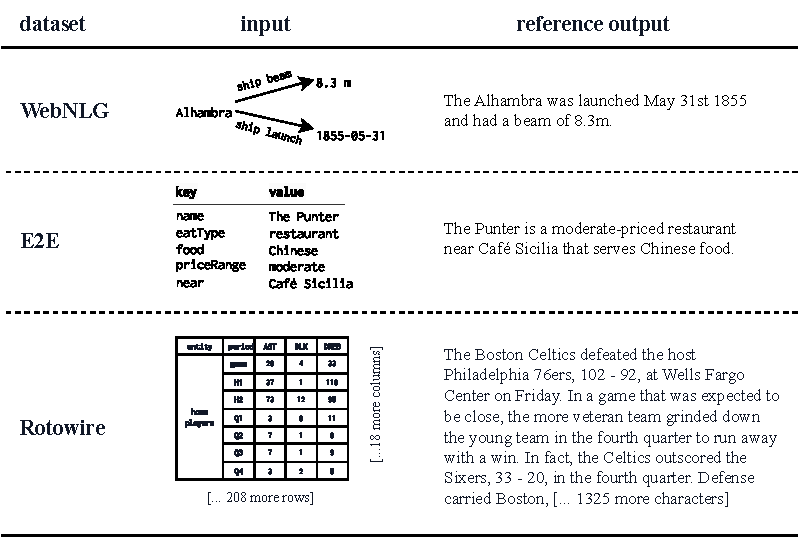
\includegraphics[width=\textwidth]{img/datasets.pdf}
    \caption[Examples from WebNLG, E2E, and Rotowire.]{Example inputs and reference outputs from the WebNLG, E2E, and Rotowire datasets.}\label{fig:datasets}
\end{figure*}

\paragraph{Datasets} The following \ac{d2t} generation datasets (highlighted in \autoref{tab:datasets}) are the most relevant for the thesis:


\begin{itemize}
    \item \textbf{WebNLG}: The WebNLG dataset \cite{gardentCreatingTrainingCorpora2017,gardentWebNLGChallengeGenerating2017} contains \ac{rdf} triples from DBPedia \cite{auer2007dbpedia} and their crowdsourced descriptions. Each example consists of 1-7 triples, forming a subgraph in the DBPedia knowledge graph. The target text should describe all the entities and the relations between them. The original WebNLG dataset \cite{gardentCreatingTrainingCorpora2017} contains 15 domains (such as Astronaut, Building, or Food), out of which 5 are \emph{unseen}, i.e., included only in the test set. Each set of triples included several verbalizations to promote lexical variability. In the version 2, the dataset has been fixed, annotated for intermediate subtasks, and enriched with semi-automated German translations \cite{shimorinaHandlingRareItems2018,castroferreiraEnrichingWebNLGCorpus2018}. Version 3 of the data \cite{ferreira20202020} contains one additional domain and automatic translations to Russian.
          \begin{itemize}
              \item
                    We participated in the 2020 edition of \emph{WebNLG Challenge}, which is a series of shared tasks based on the WebNLG dataset (\citealp{gardentWebNLGChallengeGenerating2017,shimorinaWebNLGChallengeHuman2019,ferreira20202020,cripwell2023WebNLGShared2023}; see \autoref{sec:finetuning}). We also used the dataset in the experiments on low-resource \ac{d2t} generation (\Cref{sec:iterative,sec:pipeline}), evaluation (\autoref{sec:sem-acc}), data processing (\autoref{sec:tabgenie}), and out-of-domain generalization (\autoref{sec:rel2text}).
          \end{itemize}

    \item \textbf{E2E}: The E2E dataset \cite{dusekEvaluatingStateoftheartEndtoEnd2020,dusekSemanticNoiseMatters2019} contains restaurant descriptions in the form of key-value pairs (3-8 items per example) and corresponding human-written restaurant recommendations. The name of the dataset is derived from the E2E Challenge, a shared task that focused on evaluating end-to-end \ac{d2t} generation systems \cite{dusekEvaluatingStateoftheartEndtoEnd2020}. Since the original version of the dataset was riddled with semantic noise (incorrect or missing facts in the crowdsourced descriptions), we use the cleaned version from \citet{dusekSemanticNoiseMatters2019} as the default version for our experiments.
          \begin{itemize}
              \item
                    Similarly to WebNLG, we used the dataset in our experiments on low-resource \ac{d2t} generation (\Cref{sec:iterative,sec:pipeline}), evaluation (\autoref{sec:sem-acc}), and data processing (\autoref{sec:tabgenie}).
          \end{itemize}

    \item \textbf{Rotowire}: Rotowire \cite{wiseman2017challenges} is a dataset with tabular statistics of basketball games and their corresponding game summaries. The target text contains only a small subset of the full input table, so the systems also need to model the content selection step. Together with the full-paragraph length of the target summaries, this aspect makes the dataset particularly challenging for \ac{d2t} generation systems.
          \begin{itemize}
              \item
                    We used the outputs from the neural systems on this dataset for building a token-level evaluation metric (\autoref{sec:tok-eval}). We also included its updated version SportSett:Basketball \cite{thomson2020sportsett} in our data processing toolkit (\autoref{sec:tabgenie}).
          \end{itemize}
\end{itemize}

See \autoref{fig:datasets} for example inputs and reference outputs from these datasets.

\subsection{Evaluation Metrics}
\label{sec:evaluation}

The most common evaluation measures for \ac{d2t} generation are \emph{intrinsic}, i.e., focusing on evaluating certain aspects of the quality of the system and its outputs \cite{gkatzia2015snapshot,celikyilmazEvaluationTextGeneration2021}.\footnote{As opposed to \emph{extrinsic} measures, which evaluate the impact of the system in the external environment \cite{celikyilmazEvaluationTextGeneration2021}. While \emph{extrinsic} metrics could give us a better picture of the real-world impact, they are not suitable for early research stages due to high demands on the system quality, and they are also less suitable for evaluating individual subtasks \cite{van2019best}, which is why we focus on intrinsic measures in this work.} The intrinsic measures can be divided between \emph{automatic metrics} and \emph{human evaluation}. Automatic metrics are generally cheaper, faster, and more easily replicable. However, they mostly serve only as a crude heuristic for the desired performance measure, which should be correlated with human judgment \cite{van2019best}. Human evaluation is more expensive and difficult to execute, but if executed correctly, it can give us a more precise and fine-grained picture of system performance. A rule of thumb is that an experimental result should be supported by both kinds of metrics.


If we have human-written (also called \emph{ground truth} or \emph{gold-standard}\footnote{The term \emph{gold-standard} can misleadingly suggest that human-written references are the ``holy grail'' which the systems should imitate. This is generally an overstatement, as human-written references are often noisy and faulty \cite{dusekSemanticNoiseMatters2019,clarkAllThatHuman2021}, but they can still serve as a valuable point of reference.}) reference texts at our disposal, we can use \emph{reference-based}  automatic metrics. The implicit assumption with reference-based metrics is that the more similar the generated text is to the respective human-written reference text, the better. \emph{Referenceless} metrics, on the other hand, can be more varied: they can either judge the intrinsic qualities of the text, such as its fluency, diversity, and reading level, or---taking the input data into account---the faithfulness of the text with respect to the input data. \cite{celikyilmazEvaluationTextGeneration2021}

In the following paragraphs, we will introduce  reference-based automatic metrics for measuring lexical similarity, semantic similarity, and semantic accuracy of the generated text, followed by referenceless automatic metrics for text fluency and lexical diversity. Finally, we will discuss evaluation methods based on human annotators and large language models.


\paragraph{Lexical Similarity} Lexical similarity metrics measure the similarity between the generated and reference text using word-level (or character-level) overlap. These metrics are fast, easy to compute, and have been used for decades as a convenient proxy for system comparison in various \ac{nlp} areas \cite{celikyilmazEvaluationTextGeneration2021}. However, there is a recent upsurge of works arguing against these metrics because their correlations with human judgments for high-quality outputs are low or negative, and the metrics fail to capture fine-grained phenomena \cite{mathurTangledBLEUReevaluating2020,kocmiShipNotShip2021,gehrmannRepairingCrackedFoundation2022}. As a general rule, lexical similarity metrics (if used, e.g., for comparison with prior work) should be accompanied by other metrics.

Here are some of the common metrics which we use in this work:

\begin{itemize}
    \item \textbf{BLEU} \cite{papineni2002bleu} measures $n$-gram precision, i.e., to which extent the $n$-grams in the generated text correspond to the reference text.  It is computed as a geometric mean of the individual 1-4-gram precisions, with a brevity penalty to penalize outputs shorter than the reference. \acs{bleu} was originally used for evaluating \ac{mt}, but it has become commonplace in \ac{nlp}. The SacreBLEU library \cite{post2018call}  was developed to tackle inconsistencies in implementations of the metric \cite{reiter2018structured}.
    \item \textbf{ROUGE} \cite{lin-2004-rouge} is a set of metrics that focus on recall, i.e., to which extent does the generated text preserve the information in the reference text. ROUGE has been originally designed for evaluating automatic summarization, but similarly to BLEU, it has been used widely (and as recently found by \citet{gruskyRogueScores2023}, oftentimes incorrectly) across the \ac{nlp} literature. ROUGE includes several variants, such as ROUGE-L, which measures the longest matching word sequence, and ROUGE-{1/2/3/4}, which measures the overlap on the respective $n$-grams.
    \item \textbf{METEOR} \cite{banerjee-lavie-2005-meteor} is a metric that computes the harmonic mean of precision and recall w.r.t. a reference computed on unigrams. METEOR also partially addresses non-exact matches by using stemming and synonym matching. It has been shown to produce better correlations with human judgments than \acs{bleu} \cite{agarwal2008meteor} but is more complex and expensive to compute.
    \item \textbf{NIST} \cite{martin2000nist} is a metric which focuses on precision similarly to \acs{bleu}. However, it assigns higher weights to less common n-grams, which are considered more informative \cite{doddington2002automatic}. Its length penalty is also more robust to slight variations in text length.
    \item \textbf{ChrF++} \cite{popovic2015chrf,popovic2017chrf} is a metric which computes the F1-score on \emph{character} $n$-grams. The metric is more robust to morphological variations than word-level metrics. On top of the original ChrF metric, ChrF++ also considers word unigrams and bigrams along with the character $n$-grams.
          % \item \textbf{CIDEr} \cite{vedantam2015cider} is a metric originally designed for evaluating image captions. It considers n-gram overlap, word frequency, and the informativeness of the generated caption compared to the reference captions. While not typically used for text summarization or \ac{mt} evaluation, it can be adapted for these tasks as well.
\end{itemize}
\paragraph{Semantic Similarity} As described in \autoref{sec:text-repr}, word embeddings map words with similar meanings close to each other in the vector space. Semantic similarity metrics use this fact to measure the similarity of texts as a distance between their embeddings. The metrics most often rely on \emph{contextual embeddings} computed by pretrained transformer encoders (\citealp{peters2018deep,devlinBERTPretrainingDeep2019}; see \autoref{sec:transformer}). In contrast to lexical similarity metrics, semantic similarity metrics are more robust to lexical variations but are more computationally expensive. They are also subject to limitations of pretrained models, including their biases and black-box nature.

The following are the metrics which we use in this work:

\begin{itemize}
    \item \textbf{BERTScore} \cite{zhang2019bertscore} measures the semantic similarity of texts by computing cosine similarity between the embeddings of the texts encoded by a pretrained transformer model. It was initially developed on top of BERT \cite{devlinBERTPretrainingDeep2019}, but it now also supports other transformer encoder models. Its flexibility helps to achieve better correlations with human judgment but makes it less suitable for comparison across different works.
    \item \textbf{BLEURT} \cite{sellam2020bleurt} measures semantic similarity of texts using a BERT model \cite{devlinBERTPretrainingDeep2019} which is further finetuned for predicting human ratings on synthetically labeled data. Compared to BERTScore, BLEURT is less flexible but ensures a more consistent setup across works.
    \item \textbf{NUBIA} \cite{kaneNUBIANeUralBased2020} measures semantic similarity of texts by combining features from two finetuned RoBERTa models \cite{liuRoBERTaRobustlyOptimized2019}, on the semantic similarity benchmark STS \cite{cer-etal-2017-semeval} and on the natural language inference benchmark MNLI \cite{williams2018mnli}; along with perplexity from the GPT-2 model \cite{radford2019language}. These features are combined using an \ac{mlp} layer. Combining the features ensures better robustness of the metric at the cost of higher complexity and higher computational requirements.
\end{itemize}

\paragraph{Semantic Accuracy} Semantic accuracy\footnote{The similar phenomenon is also called \emph{faithfulness}, \emph{factual accuracy}, or \emph{factual consistency} \cite{celikyilmazEvaluationTextGeneration2021}. We emphasize that in this work, we use the term \emph{semantic accuracy} to refer to the faithfulness of the text \emph{to the input data}, i.e., regardless of the factual correctness of the data itself (as opossed to \emph{factual accuracy}, which is determined by the actual state of the world).} measures inaccuracies in the output text with respect to the input data. The inaccuracies in \ac{d2t} generation can be broadly divided into \emph{omissions} (the model not mentioning facts in the input data) and \emph{hallucinations} (the model mentioning extra facts that are not supported by the input data). Naturally, omissions apply only if the task requires mentioning all the facts in the input data. Further, hallucinations can be \emph{extrinsic}, i.e., the model introduces external information not present in the data, or \emph{intrinsic}, i.e., the model uses the data incorrectly. \cite{maynezFaithfulnessFactualityAbstractive2020}

% The closest notion is the \emph{slot error rate} from task-oriented dialogue systems, which is typically implemented by exact string match or regular expressions  \cite{wen2015semantically,dusekEvaluatingStateoftheartEndtoEnd2020}. 

% Metrics for measuring semantic accuracy in \ac{d2t} generation are sparse. 
\citet{honovich2022true} presents a survey of factual consistency metrics, focusing on \ac{nlg} areas such as summarization, fact verification, paraphrasing, and knowledge-grounded dialogue. Targetting specifically \ac{d2t} generation, Data-QuestEval \cite{rebuffel2021data} is a referenceless metric that uses QuestEval \cite{scialomQuestEvalSummarizationAsks2021}, a tandem of question generation and question answering models. For tabular data, PARENT \cite{dhingraHandlingDivergentReference2019} was proposed as a reference-based metric, which uses lexical alignment models for computing precision and recall for tabular values. In \Cref{sec:sem-acc,sec:tok-eval}, we present two novel referenceless metrics for evaluating semantic accuracy of \ac{d2t} generation using \acp{plm}. In \autoref{sec:quintd}, we also show how to evaluate the semantic accuracy of texts using a \ac{llm}.

\paragraph{Text Fluency} Text fluency is a catch-all term for measuring grammatical correctness, spelling, word, and stylistical choices of text \cite{celikyilmazEvaluationTextGeneration2021}. In \ac{mt}, lexical similarity metrics (such as \acs{bleu}) were used as a proxy for measuring text fluency, following the intuition that texts that are more similar to human written text tend to be more fluent \cite{papineni2002bleu,celikyilmazEvaluationTextGeneration2021}. However, outside of \ac{mt}, the correlation between lexical similarity metrics and fluency was repeatedly found to be low or negative \cite{novikovaWhyWeNeed2017,fabbri2021summeval,nekvinda2021shades}. An alternative measure of text fluency is the \emph{perplexity} of the text under a neural \ac{lm}. This approach assumes that the \ac{lm} assigns higher probability to more fluent sentences, which were supposedly more common in the pretraining corpus. Despite its shortcomings \cite{wang2022perplexity}, this approach is used in various \ac{nlg} works \cite{kann2018sentence,wang2020cat,kaneNUBIANeUralBased2020,liu2021can,leeFactualityEnhancedLanguage2022}.


\paragraph{Lexical Diversity} Lexical diversity measures the variability and richness of expressions in the text \cite{vanmiltenburgMeasuringDiversityAutomatic2018}. One way to express lexical diversity is the ratio between the average number of different words and the total number of words, called \emph{\ac{ttr}} or \emph{distinct $n$-grams} \cite{johnson1944studies,li2016diversity}. Another way is to measure entropy of $n$-grams \cite{shannon1948mathematical}.
Lexical diversity is not generally required in \ac{d2t} generation, although there are approaches explicitly aiming to decode diverse outputs \cite{hanGeneratingDiverseDescriptions2021,perlitzDiversityEnhancedTabletoText2022}.

\paragraph{Human Evaluation} Since automatic metrics serve only as imperfect proxies for human judgment, using human annotators is a crucial part of any \ac{nlg} experimental evaluation \cite{gehrmannRepairingCrackedFoundation2022}. Although there are attempts at standardizing human evaluation \cite{thomsonGoldStandardMethodology2020}, human annotation protocols are usually task-specific \cite{van2019best,belzDisentanglingPropertiesHuman2020,howcroft2020twenty}. There are two main paradigms of human evaluation: large-scale evaluation using crowd workers mainly focusing on quantitative aspects (\emph{crowdsourcing}), and small-scale evaluation using expert annotators focusing primarily on qualitative aspects (\emph{manual evaluation}).

\begin{itemize}
    \item \textbf{Crowdsourcing}: Crowdsourcing platforms such as Amazon Mechanical Turk\footnote{\url{https://www.mturk.com}} or Prolific\footnote{\url{https://prolific.com}} are often used for distributing the work between human annotators. These platforms offer a convenient interface for hiring annotators with a specific background. Due to financial incentives and skill issues, the quality of outputs may vary, especially since the workers are nowadays prone to delegating the task to \acp{llm} \cite{veselovskyArtificialArtificialArtificial2023}. It is, therefore, necessary to employ quality assurance checks in the annotation process.
    \item \textbf{Manual Error Analysis}: To measure fine-grained aspects of output quality, manual evaluation can be performed by the paper authors or other domain experts on a moderate-sized sample of data (\textasciitilde 100 examples). The main goal of manual evaluation is to provide insights into the kinds of errors that appear in the output texts.
\end{itemize}


\paragraph{LLM-based Evaluation} Recently, researchers have started to examine the potential of replacing human annotators with \acp{llm}-based metrics \cite{zhaoInvestigatingTabletoTextGeneration2023,sottanaEvaluationMetricsEra2023,kocmiLargeLanguageModels2023,chiang-lee-2023-large,wangChatGPTGoodNLG2023a,fu2023gptscore}. In particular, the GPT-4 model \cite{openai2023gpt4} was shown to be better in following fine-grained instructions compared to other LLMs and of having high correlations with human judgment on evaluating generated texts.  Since the model can be prompted for the specific task, using \acp{llm} can be cheaper and more robust than human annotators. However, due to concerns about its non-reproducibility \cite{kocmiGEMBAMQMDetectingTranslation2023} and bias \cite{wangLargeLanguageModels2023}, this evaluation method is only experimental. We present experiments with using a \ac{llm}-based metric for text evaluation in \autoref{sec:quintd}.


\chapter{Low-Resource Data-to-Text Generation}
\label{chap:low-res}

In this chapter, we introduce three approaches for low-resource \ac{d2t} generation based on \acp{plm}. By \emph{low-resource}, we mean using as little data as possible for generating fluent and accurate text. We develop approaches that leverage the general-domain pretraining of \acp{plm} in order to generate texts in domains with thousands, hundreds, or even zero training examples.

The data we focus on are \emph{\acs{rdf} triples} from factual knowledge graphs in the WebNLG dataset and \emph{key-value meaning representations} in the E2E dataset. Both datasets were previously described in \autoref{sec:datasets}. These datasets assume that content selection was performed beforehand, i.e., we always want to verbalize the whole input.

The most straightforward setting, presented in \autoref{sec:finetuning}, consists of finetuning mBART \cite{liuMultilingualDenoisingPretraining2020}, a pretrained transformer encoder-decoder model. For finetuning the model, we need approximately thousands of in-domain examples. We show that this baseline is powerful, achieving competitive results on a shared task for generating knowledge graph descriptions. On top of that, we show that this approach generalizes to languages other than English, namely Russian.

In \Cref{sec:iterative,sec:pipeline}, we present approaches that can generate texts with an even more limited amount of in-domain training examples. Our key idea is to use a \ac{plm} only as a tool for improving text fluency \emph{regardless of the content} and delegating (possibly crude and basic, but factually correct) verbalization of the content to different, more controllable means. \autoref{sec:iterative} shows an approach based on a text-editing model, which has a limited vocabulary and is trained on iteratively fusing simple templates. The limited vocabulary and training objective helps the model to generate factually correct sentences. In \autoref{sec:pipeline}, we present an alternative approach that adds an ordering and aggregation step for generating more fluent texts. Moreover, we show how to train a \ac{plm} for all the steps entirely on general-domain operations, reducing the need for in-domain examples to zero.

\section{Finetuning Pretrained Language Models}
\label{sec:finetuning}

\begin{refbox}
    This section is based on the paper \emph{Train Hard, Finetune Easy: Multilingual Denoising for RDF-to-Text Generation} \cite{kasnerTrainHardFinetune2020}, joint work with Ondřej Dušek, published in the Proceedings of the 3rd International Workshop on Natural Language Generation from the Semantic Web (WebNLG+) at INLG 2020.
\end{refbox}


In this section, we introduce a simple approach for generating knowledge graph descriptions. Our approach is based on finetuning a multi-lingual \ac{plm} on linearized graphs and the accompanying human-written descriptions from the WebNLG dataset. In the WebNLG+ Shared Task, our model ranked in the first third of the leaderboard for English and the first or second for Russian on automatic metrics. It also made it in the best or second-best system cluster on human evaluation. Our approach shows how, with a moderate amount of finetuning data, a simple \ac{plm}-based baseline can achieve satisfactory results for the task. We also highlight the remaining shortcomings of such an approach.

\subsection{WebNLG+ Shared Task}
\label{sec:webnlgp}
The WebNLG Challenge 2020\footnote{\url{https://synalp.gitlabpages.inria.fr/webnlg-challenge/challenge_2020/}} (WebNLG+; \citealp{ferreira20202020}) was the second edition of the shared task in graph-to-text generation. The task was based on the WebNLG dataset, which contains subgraphs from the DBpedia knowledge graph. Each subgraph is described by a set of \ac{rdf} triples and accompanied with crowdsourced text descriptions (see \autoref{sec:datasets}). On top of the original challenge \cite{gardentWebNLGChallengeGenerating2017}, WebNLG+ included a separate track of generating texts in Russian, in which we also participated.


\subsection{Problem Formulation}
\label{sec:mbart}
Our input is a set of \ac{rdf} triples $x \in X$, where each triple $x = (s, p, o)$ describes the relation $p$ between the entities $s$ and $o$ in the knowledge graph. Our target output $Y$ is a fluent and semantically accurate natural language description of $X$.


We formulate the task as \emph{sequence-to-sequence} generation. First, we linearize the input sequence in the default order. We select two arbitrary separator tokens: one to delimit the contituents of the triple and another to delimit individual triples. Using the linearized sequence as an input and the target text, we finetune a pretrained encoder-decoder model using the cross-entropy objective (see \autoref{sec:transformer}). We use the finetuned model to generate the target texts using autoregressive decoding (see Algorithm~\ref{alg:decoding}).

% 


\subsection{Implementation}
\paragraph{Data Preprocessing} We use the provided XML WebNLG data reader\footnote{\url{https://gitlab.com/webnlg/corpus-reader}} to load and linearize the triples. For each triple, we use the \texttt{flat\_triple()} method which converts each triple into the ``\texttt{s $\vert$ p $\vert$ o}'' string, using a pipe (``$\vert$'') as a separator. We use another token not present in the training data (``$\blacktriangleright$'') for delimiting individual triples to avoid extending the model vocabulary.\footnote{Our choice of the separators is arbitrary, as we will adapt the model to account for our separators.
    % Works such as \TODO{cite} or \TODO{cite} show that the choice of separators is not important.
} We linearize the triples in their default order. For the input to the model, we tokenize the data using SentencePiece tokenizer \citep{kudo2018sentencepiece} trained on the training dataset, using a vocabulary of 250,000 subword tokens.

\paragraph{Model}
We use mBART \cite{liuMultilingualDenoisingPretraining2020}, a multilingual \ac{plm} based on BART, a transformer model pretrained on text denoising (see \autoref{sec:plms}).
% In pretraining, the noise function of mBART replaces text spans of arbitrary length with a mask token (35\% of the words in each instance) and permutes the order of sentences. 
The model uses 12 layers for the encoder and 12 layers for the decoder ($\sim$680M parameters), and it is pretrained on the large-scale CC25 corpus extracted from Common Crawl, which contains data in 25 languages \citep{wenzek2020ccnet}.



\paragraph{Training} We finetune the pre-trained \texttt{mbart.CC25} model from the \textsc{fairseq} toolkit \citep{ott2019fairseq} using the default parameters.\footnote{We use dropout 0.3, attention dropout 0.1, and 1024 tokens per batch. We set the initial learning rate to 0.0003 and use polynomial decay with 2500 warmup steps. We train the model using the Adam optimizer \cite{kingma2014adam} with $\beta_1=0.9, \beta_2=0.98$ and $\varepsilon=1e-06$. For the full setup, see \url{https://github.com/facebookresearch/fairseq/tree/main/examples/mbart}.} We change the total number of updates from 40k to 10k to reflect the smaller size of our data. We train a separate version of mBART for each language: $\text{mBART}_{\text{en}}$ on English inputs and English outputs, and $\text{mBART}_{\text{ru}}$ on English inputs and Russian outputs.



\subsection{Results}

\begin{table*}[t]
    \footnotesize
    \centering
    \begin{tabular}{@{}lp{12.7cm}@{}}
        \textbf{input}    & \texttt{Piotr\_Hallmann | weight | 70.308 }  $\blacktriangleright$ \texttt{ Piotr\_Hallmann | birthDate | 1987-08-25} \\
        \textbf{out (en)} & Born on August 25th 1987, Piotr Hallmann has a weight of 70.308.                                                      \\
        \midrule
        \textbf{in}       & \texttt{Ciudad\_Ayala | populationMetro | 1777539}                                                                    \\
        \textbf{out (en)} & The population metro of Ciudad Ayala is 1777539.                                                                      \\
        \midrule
        \textbf{in}       & \texttt{Bakewell\_tart | ingredient | Frangipane}                                                                     \\
        \textbf{out (ru)} & Франжипан - один из ингредиентов тарта Бейквелл.                                                                      \\[0.1cm]
        \textbf{transcr.} & Franzhipan - odin iz ingredientov tarta Bejkvell.                                                                     \\
        \textbf{transl.}  & Frangipane is one of the ingredients of the Bakewell tart.                                                            \\
    \end{tabular}
    \caption{Example outputs from the mBART model(s) finetuned for \ac{rdf}-to-text generation. (1) The model can work with unseen entities, dates and numbers. (2) The model is quite robust to unseen properties, such as \texttt{populationMetro}. However, the surface form of the property deviates too much from its meaning and the sentence is incorrect. (3) The model trained on Russian targets can use English data to form sentences in Russian, transcribing the entities to Cyrillic.}
    \label{tab:mbart:examples}
\end{table*}

We report on WebNLG automatic and human evaluation results, as well as our own error analysis.

\paragraph{Automatic Metrics}
The results of our approach for English are shown in \autoref{tab:mbart:results-en}, comparing to the baseline.
% \footnote{See \url{https://gerbil-nlg.dice-research.org/gerbil/webnlg2020results} for full results.} 
We can see that our approach beats the baseline in all metrics and places in the first third of the submissions. While it does lose performance on unseen categories, the drop is not as dramatic as for many other competing approaches.

The results for Russian are shown in \autoref{tab:mbart:results-ru}. There were fewer submissions for Russian, and our system not only beats the baseline by a large margin (as did all competing submissions), but it is able to rank first in 2 metrics out of 4 (BLEU, BERTScore) and second in the remaining ones.

\paragraph{Human Evaluation}

The challenge organizers ran a human evaluation campain, where annotators were asked to rate the texts for data coverage, relevance, correctness, text structure and fluency.  Each criterion has been rated with a number in the range from 0 (completely disagree) to 100 (completely agree). The scores were clustered into groups (1-5; 1 being the best) among which there are no statistically significant differences according to the Wilcoxon rank-sum test \citep{wilcoxon1992individual}.

Our systems placed in the top clusters (1 or 2) for both English and Russian. For English, our $\text{mBART}_{\text{en}}$ system ranks first for all the categories in \textit{seen domains}, and first or second in \textit{unseen entities} and \textit{unseen domains}. In total, our English system achieved rank 1 for relevance, correctness and text structure, and rank 2 for data coverage and fluency. For Russian, our $\text{mBART}_{\text{ru}}$ system ranks second for correctness and first in all other categories.


\begin{table*}[t]
    \footnotesize\centering
    \begin{tabular}{llcccccccccc}\toprule
                                     &          & \multicolumn{2}{c}{\bf BLEU} & \multicolumn{2}{c}{\bf METEOR} & \multicolumn{2}{c}{\bf ChrF++} & \multicolumn{2}{c}{\bf BERTScore} & \multicolumn{2}{c}{\bf BLEURT}                                     \\\midrule
        \multirow{2}{*}{All}         & Ours     & 50.34                        & (10)                           & 0.398                          & (8)                               & 0.666                          & (8)  & 0.951 & (8)  & 0.57 & (8)  \\
                                     & Baseline & 40.57                        & (14)                           & 0.373                          & (15)                              & 0.621                          & (15) & 0.943 & (14) & 0.47 & (12) \\\midrule
        \multirow{2}{*}{Seen Cat.}   & Ours     & 59.13                        & (10)                           & 0.422                          & (10)                              & 0.712                          & (9)  & 0.960 & (9)  & 0.58 & (14) \\
                                     & Baseline & 42.95                        & (31)                           & 0.387                          & (27)                              & 0.650                          & (28) & 0.943 & (31) & 0.41 & (31) \\\midrule
        \multirow{2}{*}{Unseen Cat.} & Ours     & 42.24                        & (10)                           & 0.375                          & (13)                              & 0.617                          & (10) & 0.943 & (11) & 0.52 & (10) \\
                                     & Baseline & 37.56                        & (12)                           & 0.357                          & (15)                              & 0.584                          & (15) & 0.940 & (12) & 0.44 & (12) \\\midrule
        \multirow{2}{*}{Unseen Ent.} & Ours     & 51.23                        & (4)                            & 0.406                          & (8)                               & 0.687                          & (7)  & 0.959 & (8)  & 0.63 & (8)  \\
                                     & Baseline & 40.22                        & (17)                           & 0.384                          & (15)                              & 0.648                          & (15) & 0.949 & (13) & 0.55 & (12) \\\bottomrule
    \end{tabular}
    \caption{Results of $\text{mBART}_{\text{en}}$ (all data, seen categories, unseen categories, unseen entities), compared to the baseline. The numbers in brackets show the rank of each model (out of 35 submissions) with respect to the given metric.}
    \label{tab:mbart:results-en}
\end{table*}
\begin{table*}[t]
    \footnotesize\centering
    \begin{tabular}{llcccccccc}\toprule
                 & \multicolumn{2}{c}{\bf BLEU} & \multicolumn{2}{c}{\bf METEOR} & \multicolumn{2}{c}{\bf ChrF++} & \multicolumn{2}{c}{\bf BERTScore}                               \\\midrule
        Ours     & 52.93                        & (1)                            & 0.672                          & (2)                               & 0.677 & (2)  & 0.909 & (1)  \\
        Baseline & 23.53                        & (12)                           & 0.461                          & (12)                              & 0.511 & (12) & 0.836 & (12) \\\bottomrule
    \end{tabular}
    \caption{Results of $\text{mBART}_{\text{ru}}$, compared to the baseline. The numbers in brackets show the rank of each model (out of 12 submissions) if ordered by the given metric.}
    \label{tab:mbart:results-ru}
\end{table*}

\paragraph{Manual Analysis}
To better understand the nature of errors made by our system, we manually inspected a sample of 50 outputs in each language.\footnote{Automatic back-translation to English was used to facilitate understanding of Russian.} We found factual errors in 12 English outputs, mostly concentrated along the unseen categories (\emph{Scientist}, \emph{Movie}, \emph{Musical Record}). The model tends to describe musical works and movies in terms of written works (“written”, “published” etc.), i.e., the closest seen category. There are also several swaps in roles of the entities (e.g., “is to southeast” instead of “has to its southeast”, “follows” instead of “is followed by” etc.).

In a few cases, the model hallucinates a relation not specified in the data (e.g., “born on January 1, 1934 in Istanbul” when a date of birth and current residence is given, not the birthplace) or is not able to infer background knowledge not given on the input (it talks about a dead person in the present tense).
% The swaps in roles and hallucinated relations also occured in Russian; in addition, we found a hallucinated (correct) airport name and a few forgotten ingredients for a dish from a long list. 
Factual errors in Russian were less frequent (9 sentences), which is expected as there are no unseen categories. Moreover, the system shows an impressive performance at translating entity names from the English \ac{rdf} into Russian.

We further found 10 outputs with suboptimal phrasing in English and 9 in Russian, where the model did not connect properties of the same type in a coordination (e.g., two musical genres for a record) or gave numbers without proper  units (e.g., “runtime of 89.0” or “area of 250493000000.0”).

\paragraph{Discussion}
Our solution benefits from the pretrained representations of the mBART model. Multilingual pretraining allows us to use a single architecture for both English and Russian. However, English and Russian are the two most represented languages in the mBART pre-training corpora (ca. 300 GB of data each) and the performance of our model would probably be lower with low-resource languages.

The performance of our model is also noticeably lower on categories unseen in training, and it is prone to swapping relations of entities or hallucinating relations. Even though the longest examples in the WebNLG dataset fit into the model, the length of the input sequence is still limited and the model does not generalize for inputs of arbitrary size.





\section{Iterative Sentence Fusion}
\label{sec:iterative}

\begin{refbox}
    This section is based on the paper \emph{Data-to-Text Generation with Iterative Text Editing} \cite{kasnerDatatoTextGenerationIterative2020}, joint work with Ondřej Dušek, published in the Proceedings of the 13th International Conference on Natural Language Generation (INLG 2020).
\end{refbox}

We present an approach for generating semantically accurate texts from structured data in low-resource settings. Our approach builds on a text-editing model trained on the task of \emph{sentence fusion}. We first transform individual data items to text using trivial templates, and iteratively improve the resulting text using the sentence fusion model, filtering, and re-ranking.  Our approach gets lower scores on lexical similarity metrics on WebNLG and E2E datasets than the state-of-the-art approaches; however, it achieves high levels of semantic accuracy due to the limited scope of the sentence fusion model and guaranteed presence of the entities. We also demonstrate that our task formulation opens up the possibility for zero-shot \ac{d2t} generation by training a model on a general-domain dataset for sentence fusion. The code for the experiments is available on Github.\footnote{\url{https://github.com/kasnerz/d2t_iterative_editing}}


\subsection{Motivation}
\label{sec:text-editing}
Our goal is to improve the semantic accuracy \ac{d2t} generation. Other works have pursued this goal, e.g., by adapting the decoding algorithm \cite{tianStickingFactsConfident2020}, improving robustness of the model by injecting noise in its hidden states \cite{kedzie_good_2019}, or self-training with a natural language understanding model \cite{nieSimpleRecipeReducing2019}. Our approach is inspired by the systems which use a \emph{generate-then-rerank} approach \citep{dusekSequencetoSequenceGenerationSpoken2016,juraska_deep_2018}, e.g. using a classifier \cite{harkousHaveYourText2020}, to filter incorrect outputs.

To generate outputs with sufficient semantic accuracy for the filtering step, we take advantage of three facts: (1) we can lexicalize individual data items using trivial templates, (2) concatenating the lexicalizations tends to produce an unnatural sounding but semantically accurate output, and (3) a \ac{plm} trained on improving the output fluency can be used for combining the lexicalizations.

% \textsc{LaserTagger} \cite{malmi2019lasertagger}, which we use in our approach, is a sequence tagging model based on the transformer architecture with BERT \cite{devlinBERTPretrainingDeep2019} as the encoder backbone. Other recent text-editing models without a pre-trained backbone include EditNTS \citep{dong} and Levenshtein Transformer \citep{gu2019levenshtein}.

% Concurrently with our work, \citet{kale2020few} explored using templates for dialogue response generation. %\ODdel{Unlike our work,} 
% They use the sequence-to-sequence T5 model \citep{raffel2019exploring} to generate the output text from scratch instead of iteratively editing the intermediate outputs, which leaves less control over the model.


\subsection{Method}
\label{sec:text-editing-exp}
We focus on data structured as \ac{rdf} triples.\footnote{Later, we also trivially extend our approach to key-value pairs.} In our approach, we start from single-triple templates and iteratively fuse them into the resulting text while filtering and reranking the results. We first detail the main components of our system (template extraction, sentence fusion, \ac{plm} scoring) and then give the overall description of the generation algorithm.

\begin{figure*}[t]
    \centering
    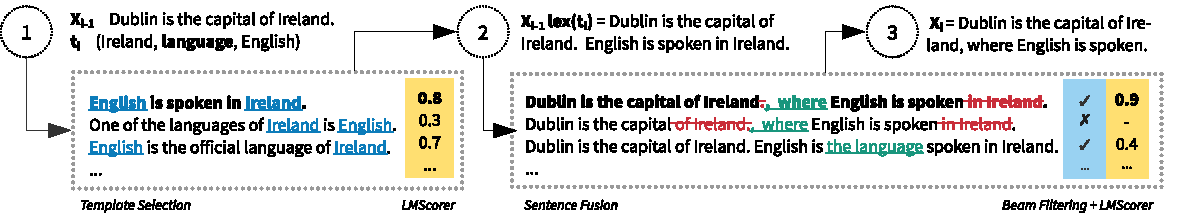
\includegraphics[width=\textwidth]{img/d2t_text_editing}
    \caption{A single iteration of our algorithm for iterative \ac{d2t} generation. In Step 1, the template for the triple is selected and filled. In Step 2, the sentence is fused with the template. In Step 3, the result for the next iteration is selected from the beam by filtering and language model scoring.}\label{fig:iterative:alg}
\end{figure*}



\paragraph{Template Extraction}
We collect a set of templates for each unique predicate. We use two approaches: (a) handcrafting the template manually for each predicate in the training set, and (b) automatically extracting the template from the lexicalizations of the examples  in the training set. For unseen predicates, we add a single fallback template: \textit{The <predicate> of <subject> is <object>.}


\paragraph{Sentence Fusion}
We train a model for the task of \emph{sentence fusion}, i.e., combining sentences into a coherent text \cite{barzilay2005sentence}.
%We train an independent in-domain sentence fusion model for each dataset. 
To construct the training data for the model, we select pairs of examples $(X, X')$ and their corresponding text descriptions $(Y, Y')$ from the original training set such that the examples consist of $(k, k+1)$ triples and have $k$ triples in common. This leaves us with an extra triple $x_{k+1}$ present only in $X'$. For each training example, we use the concatenated sequence $Y \mathrm{lex}(x_{k+1})$ as a source and the sequence $Y'$ as a target, where $\mathrm{lex}(x_{k+1})$ denotes lexicalizing the triple $x_{k+1}$ using an appropriate template.
As a result, the model learns to integrate $Y$ and $x_{k+1}$ into a single coherent expression.


\paragraph{PLM Scoring} For re-ranking the text, we use an additional component for computing text fluency, which we refer to as \textsc{LMScorer}.
As described in \autoref{sec:evaluation}, we use perplexity of the text under a a \ac{plm}, computing the score of the output text $Y$ composed of tokens $(y_1, \ldots, y_n)$ as a geometric mean of the token conditional probability:
\begin{align}
    \operatorname{score}(Y) = \Bigg( \prod_{i=1}^{n}{P(y_i|y_1, \ldots, y_{i-1})} \Bigg)^{\frac{1}{n}}.
\end{align}




\paragraph{Generation Algorithm}
The input of the algorithm (\autoref{fig:iterative:alg}) is a set of $T$ ordered triples. First, we lexicalize the triple $x_0$ to get the output text $Y_0$ by filling the available templates and using the template with the best score from \textsc{LMScorer}.
% This promotes templates which sound more natural for particular values.
In each of the following steps $i=(1, \ldots, T-1)$, we lexicalize the triple $x_i$ and concatenate it with $Y_{i-1}$.  For improving the fluency of the text, we use the sentence fusion model with beam search to produce $k$ hypotheses. We filter and re-rank the hypotheses, getting $Y_{i}$ (see the next paragraph), and proceed to the next step. The output of the algorithm is the text $Y_{T-1}$ from the final step.


\paragraph{Filtering and Re-ranking} In each decoding step, we remove hypotheses in the beam missing any entity from the input data using a simple heuristic based on string matching. Next, we rescore the remaining hypotheses in the beam with \textsc{LMScorer} and set the hypothesis with the best score as $Y_{i}$. In case there are no sentences left in the beam after the filtering step, we let $Y_{i}$ be the text in which the lexicalized $x_i$ is appended after $Y_{i-1}$ without sentence fusion, ensuring the semantic accuracy of the text.

%For the E2E dataset, we first try to find a pair of predicates for which there is a template extracted from the data, and only use the handcrafted templates for the single predicates in the subsequent steps. 
%The final beam filtering step is a simple heuristic, checking if all entities from the input triples are present in the output.


\subsection{Implementation}
\label{sec:iterative:implementation}

\begin{table}[t]
    \centering\footnotesize
    \begin{tabular}{@{}lllll@{}}
        \textbf{dataset} & \textbf{method} & \textbf{predicate}          & \textbf{example \#1}                       & \textbf{example \#2}                \\\midrule
        WebNLG           & extracted       & \texttt{foundedBy}          & \et{} was the founder of \eh{}.            & \eh{} was founded by \et{}.         \\
        E2E              & extracted       & \texttt{area}+\texttt{food} & \eh{} offers $\ets$ cuisine in the $\etf$. & \eh{} in $\etf$ serves $\ets$ food. \\
        E2E              & manual          & \texttt{near}               & \eh{} is located near \et{}.               & \et{} is close to \eh{}.
    \end{tabular}
    \caption{Examples of templates we used in our experiments. The templates for the single predicates in the WebNLG dataset and the pairs of predicates in the E2E dataset are extracted automatically from the training data; the templates for the single predicates in E2E are created manually.}
    \label{tab:iterative:templates_ex}
\end{table}


\paragraph{Template Extraction} We experiment with the WebNLG and E2E datasets (see \autoref{sec:datasets}). For WebNLG, we extract the templates from the training examples containing only a \textit{single} triple. In the E2E dataset, there are no such examples; therefore we first extract the templates for \textit{pairs} of predicates, using them as a starting point for the algorithm in order to leverage the lexical variability in the data (manually filtering out the templates with semantic noise), and we also create a small set of templates for each \textit{single} predicate manually, using them in the subsequent steps of the algorithm.\footnote{In the E2E dataset, the data is in the form of key-value pairs. We transform the data to \ac{rdf} triples by using the name of the restaurant as a \textit{subject} and the rest of the pairs as \textit{predicate} and \textit{object}. This creates \textit{n-1} triples for \textit{n} pairs.} See \autoref{tab:iterative:templates_ex} for examples of templates we used in our experiments.

\paragraph{Sentence Fusion Model} We base our sentence fusion model on the text-editing model \textsc{LaserTagger} \cite{malmi2019lasertagger}. \textsc{LaserTagger} generates outputs by tagging inputs with edit operations (\texttt{KEEP} a token, \texttt{DELETE} a token, and \texttt{ADD} a phrase before the token), which makes it suitable for tasks where the output highly overlaps with the input. An important feature of \textsc{LaserTagger} is the limited size of its vocabulary, which consists of $l$ most frequent (possibly multi-token) phrases used to transform inputs to outputs in the training data. After the vocabulary is precomputed, all infeasible examples in the training data are filtered out. At the cost of limiting the number of training examples, this filtering makes the training data cleaner by removing outliers. The limited vocabulary also makes the model less prone to hallucinations errors.

\paragraph{LMScorer} As the \textsc{LMScorer} backend, we use the pre-trained GPT-2 language model \citep{radford2019language} from the Transformers repository\footnote{\url{https://github.com/huggingface/transformers}} \citep{wolf2019HuggingFacesTS}. We compute the perplexity scores using the \textit{lm-scorer}\footnote{\url{https://github.com/simonepri/lm-scorer}} package.





\begin{table*}[t]% \begin{adjustbox}{max width=\textwidth}
    \centering\footnotesize
    \begin{tabular}{lcccc<{\hspace{2mm}}c>{\hspace{2mm}}cccc} \toprule
                         & \multicolumn{4}{c}{\bf WebNLG} &            & \multicolumn{4}{c}{\bf E2E}                                                                                                                                                                          \\
        \cmidrule{2-5} \cmidrule{7-10}
                         & {\it BLEU}                     & {\it NIST} & \hspace{-1mm}{\it METEOR}\hspace{-1mm} & \hspace{-1mm}{\it ROUGE$_L$}\hspace{-1mm} &  & {\it BLEU} & {\it NIST} & \hspace{-1mm}{\it METEOR}\hspace{-1mm} & \hspace{-1mm}{\it ROUGE$_L$}\hspace{-1mm} \\
        {\bf baseline}   & 0.277                          & 6.328      & 0.379                                  & 0.524                                     &  & 0.207      & 3.679      & 0.334                                  & 0.401                                     \\
        {\bf zero-shot } & 0.288                          & 6.677      & 0.385                                  & 0.530                                     &  & 0.220      & 3.941      & 0.340                                  & 0.408                                     \\
        {\bf w/fusion }  & 0.353                          & 7.923      & 0.386                                  & 0.555                                     &  & 0.252      & 4.460      & 0.338                                  & 0.436                                     \\
        {\bf SFC }       & 0.524                          & -          & 0.424                                  & 0.660                                     &  & 0.436      & -          & 0.390                                  & 0.575                                     \\
        {\bf T5 }        & 0.571                          & -          & 0.440                                  & -                                         &  & -          & -          & -                                      & -                                         \\ \bottomrule
    \end{tabular}
    \caption{Results of automatic metrics on the WebNLG and E2E test sets. The comparison is made with the results from the papers on the Semantic Fidelity Classifier (SFC; \citealp{harkousHaveYourText2020}) and the finetuned T5 model (T5; \citealp{kaleTexttoTextPreTrainingDatatoText2020}), state-of-the-art approaches at that time.}
    \label{tab:results}
    % \end{adjustbox}
\end{table*}



\subsection{Experiments}
\paragraph{Base Experiments} As a \emph{baseline}, we generate the best templates according to \textsc{LMScorer} without applying the sentence fusion (i.e., always using the fallback). For the \emph{sentence fusion} experiments, we use \textsc{LaserTagger} with the autoregressive decoder with a beam of size 10. We use all reference lexicalizations and the vocabulary size $V=100$, following our preliminary experiments. We finetune the model for 10,000 updates with batch size 32 and learning rate $2 \times 10^{-5}$.
For the beam filtering heuristic, we check for the presence of entities by simple string matching in WebNLG; for the E2E dataset, we use a set of regular expressions from \citet{dusekSemanticNoiseMatters2019}. We process the triples in their default order.

\paragraph{Zero-shot Experiment} Additionally, we conduct a \textit{zero-shot} experiment. We train the sentence fusion model with the same setup, but instead of the in-domain datasets, we use a subset of the balanced-Wikipedia portion of the \textsc{DiscoFuse} dataset \cite{geva-etal-2019-discofuse}. In particular, we use the discourse types which frequently occur in our datasets, filtering the discourse types which are not relevant for our use-case.


% \vspace{-3mm}
\subsection{Results}

\begin{table*}[t] \footnotesize
    \begin{tabular}{l p{12cm}}
        \textbf{Triples}   & \textit{(Albert Jennings Fountain, deathPlace, New Mexico Territory); (Albert Jennings Fountain, birthPlace, New York City); (Albert Jennings Fountain, birthPlace, Staten Island)} \\ \midrule
        \textbf{Step \#0}  & Albert Jennings Fountain died in New Mexico Territory.                                                                                                                              \\
        \textbf{Step \#1}  & Albert Jennings Fountain, who died in New Mexico Territory, was born in \greenund{New York City}.                                                                                   \\
        \textbf{Step \#2}  & Albert Jennings Fountain, who died in New Mexico Territory, was born in New York City, \greenund{Staten Island}.                                                                    \\ \midrule
        \textbf{Reference} & Albert Jennings Fountain was born in Staten Island, New York City and died in the New Mexico Territory.
    \end{tabular}
    \caption{An example of correct behavior of the algorithm on the WebNLG dataset. Newly added entities are underlined, the output from Step \#2 is the output text.}\label{tab:iterative:output}
\end{table*}


\paragraph{Accuracy vs.\ Fluency}
The scores from the automatic metrics lag behind the state-of-the-art, although both the fusion and the zero-shot approaches show improvements over the baseline. Our approach ensures zero entity errors, since the entities are filled verbatim into the templates and in case an entity is missing in the whole beam, a fallback is used instead. Semantic inconsistencies still occur, e.g.\ if a verb or function words are missing.

The fused sentences in the E2E dataset, where all the objects are related to a single subject, often lean towards compact forms, e.g.: \textit{Aromi is a family friendly chinese coffee shop with a low customer rating in riverside}. On the contrary, the sentence structure in WebNLG mostly follows the structure from the templates and the model performs minimal changes to fuse the sentences together. See \autoref{tab:iterative:output} for examples of the system outputs. Out of all steps, 28\% are fallbacks (no fusion is performed) in WebNLG and 54\% in the E2E dataset. % v anglictine se za '\%' nedela mezera
The higher number of fallbacks in the E2E dataset can be explained by a higher lexical variability of the references, together with a higher number of data items per example in the E2E dataset, making it harder for the model to maintain the text coherency over multiple steps.

\paragraph{Templates} On average, there are 12.4 templates per predicate in WebNLG and 8.3 in the E2E dataset. In cases where the set of templates is more diverse, e.g.\ if the template for the predicate \textit{country} has to be selected from \{\textit{<subject> is situated within <object>, <subject> is a dish found in <object>}\}, \textsc{LMScorer} helps to select the semantically accurate template for the specific entities. The literal copying of entities can be too rigid in some cases, e.g.\ \textit{Atatürk Monument (İzmir) is made of ``Bronze''}, but these disfluencies can be improved in the fusion step.

\paragraph{Reordering} \textsc{LaserTagger} does not allow arbitrary reordering of words in the sentence, which can limit the expressiveness of the sentence fusion model. Consider the example in \autoref{fig:iterative:alg}: in order to create a sentence \textit{English is spoken in Dublin, the capital of Ireland}, the model has to delete and re-insert at least one of the entities, e.g.\ \textit{English}, which has to be present in the vocabulary.

\paragraph{Domain Independence} The zero-shot model trained on \textsc{DiscoFuse} is able to correctly pronominalize or delete repeated entities and join the sentences with conjunctives, e.g.\ \textit{William Anders was born in British Hong Kong\underline{, and was} a member of the crew of Apollo 8}. While the model makes only a limited use of sentence fusion, it makes the output more fluent while keeping strong guarantees of the output accuracy.

\subsection{Discussion}
% Building a high-quality sentence fusion model, which lies at the core of our approach, remains a challenge \cite{lebanoff2020learning}. Our simple extractive approach relying on existing D2T datasets may not produce sufficient amount of clean data. On the other hand, the phenomena covered in the \textsc{DiscoFuse} dataset are too narrow for the fully general sentence fusion. We believe that training the sentence fusion model on a larger and more diverse sentence fusion dataset, built e.g. in an unsupervised fashion \cite{lebanoff-etal-2019-scoring}, is a way to improve the robustness of our approach.

% Fluency of the output sentences may be also improved by allowing more flexibility for the order of entities, either by including an ordering step in the pipeline \citep{moryossef2019astep}, or by using a text-editing model that is capable of explicit reordering of words in the sentence \cite{mallinson2020felix}. Splitting the data into smaller batches (i.e. setting an upper bound for the number of sentences fused together) could also help to improve the consistency of results with a higher number of data items.

% Our string matching heuristic is quite crude and may lead to a high number of fallbacks. Introducing a more precise heuristic, such as a semantic fidelity classifier \citep{harkous2020have}, or a model trained for natural language inference \citep{dusek2020nli} could help to promote lexical variability of the text.

% Finally, we note that the text-editing paradigm allows to visualize the changes made by the model, introducing the option to accept or reject the changes at each step, and even build a set of custom rules on top of the individual edit operations based on the affected tokens. This flexibility could be useful for tweaking the model manually for a production system.


% \subsection{Conclusions}
% We proposed a simple and intuitive approach for D2T generation, splitting the process into two steps: lexicalization of data and improving the text fluency. A trivial lexicalization helps to promote fidelity and domain independence while delegating the subtle work with language to neural models allows to benefit from the power of general-domain pre-training. While a straightforward application of this approach on the WebNLG and E2E datasets does not produce state-of-the-art results in terms of automatic metrics, the results still show considerable improvements above the baseline. We provided insights into the behavior of the model, highlighted its potential benefits, and proposed the directions for further improvements.


\section{Pipeline of Text-to-Text Neural Modules}
\label{sec:pipeline}
\begin{refbox}
    This section is based on the paper \emph{Neural Pipeline for Zero-Shot Data-to-Text Generation} \cite{kasner2022neural}, joint work with Ondřej Dušek, published in the Proceedings of the 60th Annual Meeting of the Association for Computational Linguistics (ACL 2022).
\end{refbox}

In this section, we further develop the approach from \autoref{sec:iterative} for generating semantically accurate text from structured data. The main limitation of the previous approach, which was based on iterative transformations of simple templates, was the limited fluency of the output texts. To improve text fluency, we propose adding ordering and aggregation, making the process a three-step pipeline. We also propose a way to make each of these steps trainable on a generic synthetic corpus. We confirm that on WebNLG and E2E dataset, our approach can get lower rates of omissions and hallucinations than prior approaches according to a semantic accuracy metric, while achieving levels of lexical similarity comparable to some of the prior systems; all of this without the need for in-domain training data. Our code and data is available on Github.\footnote{\url{https://github.com/kasnerz/zeroshot-d2t-pipeline}}

% an approach for transforming the templates based on a sequence of modules trained on general-domain text-based operations: ordering, aggregation, and paragraph compression. We train \acp{plm} for performing these operations on a synthetic corpus \textsc{WikiFluent} which we build from English Wikipedia. Our experiments on WebNLG and E2E show that our approach enables \ac{d2t} generation from \ac{rdf} triples in zero-shot settings. Our code and data is available on Github.\footnote{\url{https://github.com/kasnerz/zeroshot-d2t-pipeline}}

\subsection{Motivation}
Our experiments in \autoref{sec:iterative} with iterative sentence fusion led to several observations:

\begin{enumerate}
    \item The fixed order of triples limits the expressivity of the model, leading to unnatural outputs.
    \item Using the sentence fusion model on every sentence boundary tends to produce sentences which are too compact.
    \item Text-editing models underperform state-of-the-art autoregressive models in terms of output quality \cite{kaleTexttoTextPreTrainingDatatoText2020,ribeiroInvestigatingPretrainedLanguage2020}.
\end{enumerate}

Following these observations, we improve our approach by (1) inserting a triple-ordering step in the process, (2) replacing the sentence fusion by paragraph compression, and (3) basing the approach on trainable autoregressive models.


Our approach follows the idea of pipeline-based approaches (see \autoref{sec:d2t-pipeline}). In particular, our pipeline follow the idea of pipelines based on iterative improvements of simple templates  \cite{laha2020scalable} and neural modules \cite{ferreiraNeuralDatatotextGeneration2019}. We focus on the \emph{ordering} and \emph{aggregation} steps, which were shown to improve the quality of \ac{d2t} generation outputs in domain-specific setups \cite{moryossef2019improving,moryossef2019step,trisedyaSentenceGenerationEntity2020,su2021plan}.

In contrast to previous approaches, our pipeline is fully trainable on general-domain data, i.e., without using any training data from target \ac{d2t} datasets. By eliminating the need for human references, we get rid of the costly and time-consuming reference collection process. At the same time, we also avoid the brittleness of few-shot approaches, which are sensitive to the choice of finetuning examples \cite{chenFewShotNLGPreTrained2019,suFewShotTabletoTextGeneration2021,changSelectGenChallengeFinding2021}.

\subsection{Method}
\label{sec:pipeline:method}
\begin{figure}[t]
    \centering
    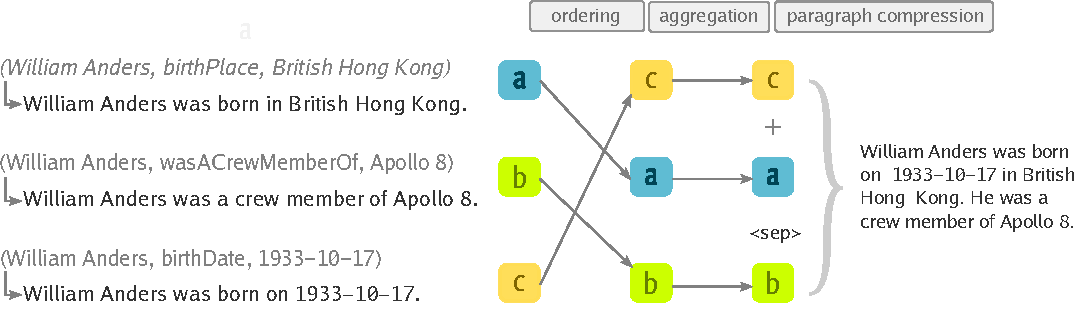
\includegraphics[width=\textwidth]{img/zeroshot_pipeline.pdf}
    \caption{A scheme of our approach for zero-shot data-to-text generation from RDF triples. After a simple transformation of triples to facts, we apply the pipeline of modules for (1) ordering, (2) aggregation, (3) paragraph compression. Individual modules are trained on a large general-domain text corpus and operate over text in natural language. In-domain knowledge is included only in the simple hand-crafted templates for each predicate.}\label{fig:zeroshot:pipeline}
\end{figure}
Here, we provide the formal description of our approach. Similarly to \Cref{sec:finetuning,sec:iterative}, we focus on the task of producing a natural language description $Y$ a set of \ac{rdf} triples $x \in X$, where each triple $x = (s, p, o)$ describes the relation $p$ between the entities $s$ and $o$ in the knowledge graph.

Given a set of triples $X$ on the input, we:
\begin{enumerate}
    \item transform the triples into \textit{facts}, which are short sentences in natural language,
    \item sort the facts using an \textit{ordering} module,
    \item insert sentence delimiters between the sorted facts using an \textit{aggregation} module,
    \item input the ordered sequence of facts with delimiters into a \textit{paragraph compression} module, which generates the final description $Y$.
\end{enumerate}

\paragraph{Transforming Triples to Facts}

The first step in our pipeline involves transforming each of the input triples $x \in X$ into a fact $f \in F$  using a transformation $T: X \rightarrow F$. We define a fact $f$ as a single sentence in natural language describing $x$.
The transformation serves two purposes: (a) preparing the data for the subsequent text-to-text operations, (b) introducing in-domain knowledge about the semantics of individual predicates.


% This step can be realized e.g. using a simple template for each predicate (cf. §\ref{sec:templates_model}).
% Several neural methods for this task were proposed, using either interactions between pairs of sentences \cite{chen2016neural,li2017neural}, global interactions \cite{gong2016end,wang2019hierarchical}, or combination of both \cite{cui2020bert}. We base our ordering module (§\ref{sec:ord_model}) on the recent work of \citet{calizzano2021ordering}, who use a pointer network \cite{wang2019hierarchical,vinyals2015pointer} on top of a PLM.


\paragraph{Ordering} We assume that the default order of triples $X$ is random. Note, however, that $F$ is a set of meaningful sentences. We can use this to our advantage and apply a sentence ordering module \cite{barzilay2001sentence,lapata2003probabilistic} maximize the coherency of the paragraph resulting from their concatenation. The sentence ordering module $O(F)$ produces an ordered sequence of facts: $F_o = \{f_{o_1}, \ldots, f_{o_n}\}$, where $o_{1:n}$ is a permutation of fact indices. An example outcome of such operation may be grouping together facts mentioning \textit{birth date} and \textit{birth place} of a person, followed by their \textit{occupation}, as it is shown in \autoref{fig:zeroshot:pipeline}. The ordering module allows downstream modules to only focus on operations over neighboring sentences.


\paragraph{Aggregation} Some facts will be typically mentioned together in a single sentence. Considering the previous example, \textit{occupation} is likely to be mentioned separately, while \textit{birth date} and \textit{birth place} are likely to be mentioned together. We make these decisions using the aggregation module, which takes a sequence of ordered facts $F_o$ as input and produces a sequence of sentence delimiters $A(F_o) = \{\delta_{o_1}, \delta_{o_2}, \ldots, \delta_{o_{n-1}}\}$; $\delta_{i} \in \{0, 1\}$.
% The output $\delta_{i}=1$ means that the neighboring facts should be mentioned separately, i.e. the neighboring sentences should \textit{not} be fused. Conversely, 
Unlike previous works \cite{wiseman2018learning,shao-etal-2019-long,shen-etal-2020-neural,xuAGGGENOrderingAggregating2021}, which capture the segments corresponding to individual parts of the input as latent variables, we simply insert delimiters into the ordered sequence of facts to mark sentence boundaries. The output $\delta_{i}=0$ means that the facts should be aggregated and their corresponding sentences should be fused. Note that the markers serve only a hint for the paragraph compression module, i.e., the sentences are not fused in this step.



\paragraph{Paragraph Compression}  The \ac{pc} module takes as input the ordered sequence of facts with delimiters $F_a = \{f_{o_1}, \delta_{o_1}, f_{o_2}, \ldots, \delta_{o_{n-1}}, f_{o_n}\}$ and produces the final text $Y$.  It has two main objectives: (a) \textit{fusing} related sentences, i.e., sentences $i$ and $j$ in between which $\delta_{i}=0$, and (b) \textit{rephrasing} the text to improve its fluency, e.g., fixing disfluencies in the templates or replacing noun phrases with refering expressions. Unlike in text summarization or sentence simplification, the edits will typically be minor, since we aim to preserve the semantics of the text.



\subsection{\textsc{WikiFluent} Corpus}
\label{sec:pipeline:wikifluent}
For training the modules, we need to build a corpus in which (1) the input is a set of simple, template-like sentences, (2) the output is a fluent text in natural language preserving the semantics of the input. Here, we propose a way how to build such a large-scale synthetic corpus from English Wikipedia. Our resulting corpus (\textsc{WikiFluent}) is orders of magnitude larger than the in-domain \ac{d2t} datasets and provides training data for all the modules in our pipeline.

% we collect a large-scale synthetic corpus \textsc{WikiFluent}. Our goal is to build a corpus covering a broad range of domains and capturing the sentence style in D2T generation. In other words, we . As we describe below in detail, we achieve that by using human-written paragraphs in English Wikipedia and applying \textit{split-and-rephrase} and  \textit{coreference resolution} models to obtain synthetic source texts. The process is illustrated in Figure \ref{fig:wikifluent}; corpus statistics are included in Appendix \ref{app:stats}.

\paragraph{Data Source} For building the \textsc{WikiFluent} corpus, we first extracted 934k first paragraphs of articles from a Wikipedia dump\footnote{\texttt{enwiki-20210401-pages-articles-multistream}} using WikiExtractor \cite{Wikiextractor2015}. Wikipedia is commonly used for large-scale pretraining of D2T generation models, as it provides a source of neutral texts based on factual data \cite{jinGenWikiDatasetMillion2020,chenKGPTKnowledgeGroundedPreTraining2020}.
% Although it is not bias-free, it provides more balanced sample of natural language use than typical D2T generation datasets. 
We used the first paragraphs of Wikipedia entries with length between 30-430 characters; filtering out lists, disambiguations, and malformed paragraphs. To balance the length of inputs, we divided the paragraphs according to their length into 4 equally-sized bins (30-130 characters, etc.) and selected 250k examples from each bin.



\begin{figure}[t]
    \centering
    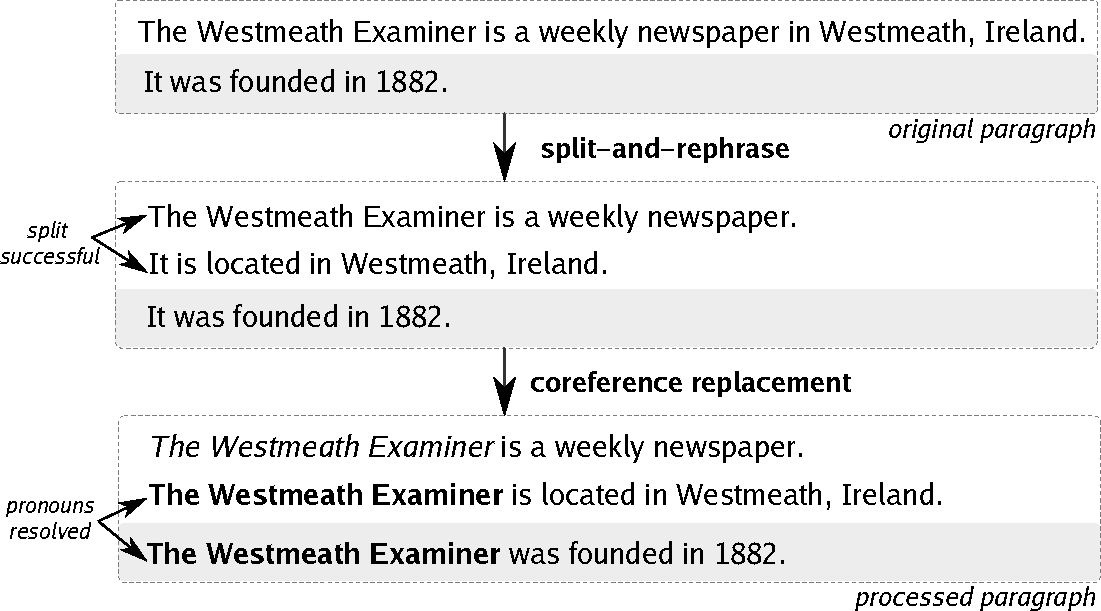
\includegraphics[width=0.7\textwidth]{img/wikifluent.pdf}
    \caption{The building process of the \textsc{WikiFluent} corpus. We apply a split-and-rephrase model on each sentence in the paragraph and resolve coreferences in the split sentences. The result is a set of simple sentences which together convey the same meaning as the original paragraph. The synthesized sentences are used as \textit{input} into our models, the original human-written texts are used as \textit{ground truth}.}\label{fig:wikifluent}
\end{figure}

\begin{table*}[t]
    \centering
    \footnotesize
    \begin{tabular}{l rrrrrrrr}\toprule
                                              & \bf  \#train & \bf \#dev & \bf \#test & \bf tok/src & \bf tok/tgt & \bf sent/src & \bf sent/tgt \\  \midrule
        WebNLG                                & 18,102       & 870       & 1,862      & 26.8        & 22.6        & 3.0          & 1.4          \\
        Clean E2E                             & 33,236       & 4,299     & 1,847      & 29.2        & 22.3        & 4.2          & 1.5          \\ \midrule
        \textsc{WikiFluent}-\textit{full}     & 915,855      & 9,346     & 9,346      & 52.9        & 41.1        & 3.9          & 2.0          \\
        \textsc{WikiFluent}-\textit{filtered} & 700,517      & 7,149     & 7,149      & 45.6        & 35.4        & 3.4          & 1.8          \\ \bottomrule
    \end{tabular}
    \caption{Number of examples (train / dev / test), average number of tokens per source and target, average number of sentences per source and target (after filling the templates for the D2T datasets), total number of templates.}
    \label{tab:stats}
\end{table*}

\paragraph{Split-and-Rephrase} Split-and-rephrase is a task of splitting a complex sentence into a sequence of shorter sentences preserving the original meaning \citep{narayan-etal-2017-split}. We train\footnote{Following the same setup as for a paragraph compression model (\autoref{sec:pipeline:implementation}).} BART-base \cite{lewisBARTDenoisingSequencetoSequence2019} for the split-and-rephrase task on the WikiSplit corpus, containing human-made sentence splits from Wikipedia edit history \cite{botha-etal-2018-learning}.  We split each paragraph into sentences using NLTK \cite{bird2006nltk} and apply the split-and-rephrase model on each sentence. To ensure that the splits are not deterministic, we choose uniformly randomly choosing between 0-2 recursive calls. If the sentence cannot be meaningfully split, the model tends to duplicate the sentence on the output; in that case, we use only the original sentence and do not proceed with the splitting.


%  apply a \textit{split-and-rephrase} on each sentence in our paragraph paragraph into sentences and apply a  model on each sentence.  To generate a set of simple template-like sentences from the Wikipedia paragraphs, we divide each  The process is illustrated in the upper part of Figure \ref{fig:wikifluent}.



\paragraph{Coreference Replacement} Unlike the templates, which always mention a single fact, the split sentences will heavily use referring expressions. To match the sentence style, we apply a coreference resolution model \cite{Lee2018HigherorderCR} from the AllenNLP framework \cite{gardner2018allennlp}. We use the model in order to replace referring expressions with their antencendents (e.g., pronouns with noun phrases). Note that we replace the referring expressions only in the synthesized sentences, not in the original paragraphs, so that the paragraph compression module is later implicitly trained to generate referring expressions in the final description.

\paragraph{Filtering} To ensure that the generated sentences convey the same semantics as the original paragraph, we use a pretrained RoBERTa model\footnote{\url{https://huggingface.co/roberta-large-mnli}} \cite{liuRoBERTaRobustlyOptimized2019} trained on the MultiNLI dataset \cite{williams2018mnli} for checking the semantic accuracy of the generated text. Following \citet{dusekEvaluatingSemanticAccuracy2020}, we test if the original paragraph entails each of the synthesized sentences (checking for omissions), and if the set of concatenated synthesized sentences entails the original paragraph (checking for hallucinations). In a filtered version of the \textsc{WikiFluent} corpus, we include only the examples without omissions or hallucinations (as computed by the model), reducing it to 714k examples (approximately 75\% of the original size).

\subsection{Implementation}
\label{sec:pipeline:implementation}

In this section, we describe how we implement our pipeline modules using simple template transformations and neural models trained on the \textsc{WikiFluent} dataset.

\begin{figure*}[t]
    \centering
    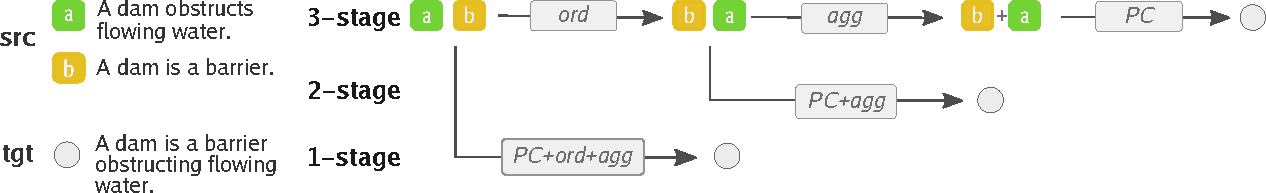
\includegraphics[width=\textwidth]{img/pipeline-variants.pdf}

    \caption{An example illustrating how the individual modules are trained and subsequently applied as the parts of the pipeline. See \autoref{sec:pipeline:implementation} for the description of the ordering model (\textsc{ord}), the aggregation model (\textsc{agg}), and the variants of the paragraph compression model (\textsc{PC, PC+agg, PC+ord+agg}).}
    \label{fig:pipeline:variants}
\end{figure*}

\paragraph{Templates}
We transform triples into facts using a single-triple template $t_i$ for each predicate, analogically to our approach in \autoref{sec:iterative:implementation}. Compared to more complex rule-based template generation engines \cite{laha2020scalable,heidari2021getting,mehta2021improving}, the approach minimizes manual workload and makes it easier to control the quality of the input for the subsequent steps.

\paragraph{Ordering Model}
For our ordering model, we use the \emph{Simple Pointer} model from \citet{calizzano2021ordering}\footnote{For details about the model, please refer to \citet{calizzano2021ordering}}. The model is based on a pretrained BART-base model \cite{lewisBARTDenoisingSequencetoSequence2019} extended with a pointer network from \citet{wang2019hierarchical}. We train the model using the synthesized simple sentences in the \textsc{WikiFluent} corpus, randomly shuffling the order of the sentences and training the model to restore their original order.

% In the encoding phase, facts $F$ are concatenated and tokenized. Each fact is surrounded by special tokens denoting the beginning (\texttt{<s>}) and the end (\texttt{</s>}) of the fact. The sequence is processed by the BART encoder, generating a sequence of encoder states $E$ for each end token \texttt{</s>} representing the preceding fact.

% The decoding proceeds autoregressively. To bootstrap the decoding process, the pair of tokens \texttt{<s></s>} is fed into the decoder, producing the decoder state $d_1$. The pointer network (attending to $d_1$ and $E$), selects the first ordered fact $f_{o_1}$, which is fed into the decoder in the next step ($d_2 = $\texttt{<s>$f_{o_1}$</s>}). The process is repeated until the all the facts are decoded in a particular order.

% The pointer network computes the probability of a fact to be on the $j$-th position, using the encoder output $E$ and the decoder output state $d_j$. The network is based on the scaled dot product attention, where $d_j$ is the query and encoder outputs $E_i$ are the keys:
% \begin{gather*}
%     Q = d_j W_Q \\
%     K = E W_K \\
%     P_{j} = \operatorname{softmax}\left(\frac{QK^T}{\sqrt{b}}\right).
% \end{gather*}
% Here $W_Q$ and $W_K \in \mathbb{R}^{b\times b}$, $b$ is the dimension of BART hidden states, and $P_{j} \in \mathbb{R}^{n+1}$ is the probability distribution for the $j$-th position (i.e., $P_{ji}$ is the probability that fact $f_i$ is on the $j$-th position).



\paragraph{Aggregation Model}
We base our aggregation model on RoBERTa-large \cite{liuRoBERTaRobustlyOptimized2019} with a token classification head. We input the sequence of ordered facts $F_o$ into the model, separating each pair of facts $f_{o_i}$ with a separator token. The token classification layer classifies each separator token into two classes $\{0,1\}$ corresponding to the delimiter $\delta_i$. We ignore the outputs for the non-separator tokens while computing cross-entropy loss. We create the training examples using the synthesized sentences in the \textsc{WikiFluent} corpus, in which we set $\delta_i=0$ for the sentences $i,i+1$ which were originally aggregated (i.e., are the result of splitting a single sentence) and $\delta_i=1$ otherwise.

\paragraph{Paragraph Compression Model} For the paragraph compression model, we finetune BART-base \cite{lewisBARTDenoisingSequencetoSequence2019} on the \textsc{WikiFluent} corpus, concatenating the synthesized sentences on the input. We add delimiters between the sentences $i$ and $i+1$ where $\delta_i=1$ using a special token \texttt{<sep>}, which we add to the model vocabulary. We expect that the model will learn to fuse the sentences between which there are no delimiters on the input. We evaluate how the model learns to respect the order and aggregation markers in \autoref{sec:pipeline:eval}.


\subsection{Experiments}
\label{sec:pipeline:experiments}
We train our pipeline modules on the \textsc{WikiFluent} corpus as described in \autoref{sec:pipeline:implementation}. Next, we use these modules \textit{without any further finetuning} for generating descriptions for RDF triples on the WebNLG and E2E datasets.

\paragraph{Pipeline versions} In order to evaluate individual components of our pipeline, we train three versions of the \textit{paragraph compression} model. The models share the same architecture and targets, but differ in their inputs:
\begin{itemize}
    \item \textsc{\ac{pc}} -- the model takes as an input ordered facts with delimiters (as described in \autoref{sec:pipeline:method}),
    \item \textsc{\ac{pc}+agg} -- the model takes as an input ordered facts \textit{without} delimiters (i.e., the aggregation is left implicitly to the model),
    \item \textsc{\ac{pc}+ord+agg} -- the model takes as an input facts in \textit{random} order and \textit{without} delimiters (i.e., both ordering and aggregation are left implicitly to the model).
\end{itemize}
Correspondingly, we test three versions of the pipeline for the \textbf{ablation study}:
\begin{itemize}
    \item \textsc{3-stage} -- a full version of the pipeline consisting of the ordering model (\textsc{ord}), the aggregation model (\textsc{agg}) and the \textsc{\ac{pc}} model,
    \item \textsc{2-stage} -- a pipeline consisting of the \textsc{ord} model and the \textsc{\ac{pc}+agg} model,
    \item \textsc{1-stage} -- a single stage consisting of the \textsc{\ac{pc}+ord+agg} model.
\end{itemize}
We evaluate all versions of the pipeline with PC models trained on the \textit{full} and \textit{filtered} versions of the \textsc{WikiFluent} dataset (see §\ref{sec:pipeline:wikifluent}).


\subsection{Evaluation}
\label{sec:pipeline:eval}
We evaluate outputs from the \textsc{\{1,2,3\}-stage} variants of our pipeline using automatic metrics, and we perform a detailed manual error analysis of the model outputs. We also evaluate the performance of the content planning modules and the ability of the PC module to follow the content plan. Finally, we include an intrinsic evaluation of our modules on the \textsc{WikiFluent} test set.

\begin{table*}[t]\centering\footnotesize
    \begin{tabular}{l p{12.2cm}} \toprule
        \textbf{Input}  & \textit{(Allen Forrest; background; solo singer), (Allen Forrest; genre; Pop music), (Allen Forrest; birthPlace; Dothan, Alabama)} \\
        \textbf{Templ.} & Allen Forrest is a solo singer. Allen Forrest performs Pop music. Allen Forrest was born in Dothan, Alabama.                       \\
        \textbf{Model}  & \lightblue{Allen Forrest is a solo singer who performs Pop music. He was born in Dothan, Alabama.}                                 \\
        \textbf{Human}  & Born in Dothan, Alabama, Allen Forrest has a background as a solo singer and was a pop artist.                                     \\\cdashlinelr{1-2}
        \textbf{Input}  & \textit{name[Wildwood], eatType[restaurant], food[French], area[riverside], near[Raja Indian Cuisine]}                             \\
        \textbf{Templ.} & Wildwood is a restaurant. Wildwood serves French food. Wildwood is in the riverside. Wildwood is near Raja Indian Cuisine.         \\
        \textbf{Model}  & \lightblue{Wildwood is a restaurant serving French food. It is in the riverside near Raja Indian Cuisine.}                         \\
        \textbf{Human}  & A amazing French restaurant is called the Wildwood. The restaurant is near the Raja Indian Cuisine in riverside. They love kids.   \\ \bottomrule
    \end{tabular}
    \caption{Example outputs of our model (\textsc{3-stage}, filtered).}
    \label{tab:pipeline:ex1}
\end{table*}

\paragraph{Automatic Metrics}


\begin{table}[t]

    \centering \small
    \begin{tabular}{llcccccccc} \toprule
                                                                                       &                  & \multicolumn{4}{c}{\textbf{WebNLG}} & \multicolumn{4}{c}{\textbf{E2E}}                                                                                                       \\
                                                                                       &                  & \textbf{B}                          & \textbf{M}                       & \textbf{O}     & \textbf{H}     & \textbf{B}     & \textbf{M}     & \textbf{O}     & \textbf{H}     \\\midrule
        \multicolumn{2}{l}{\baselinecopy{}}                                            & 37.18            & 38.77                               & 0.000                            & 0.000          & 24.19          & 34.89          & 0.000          & 0.000                           \\\cdashlinelr{1-10}
        \multicolumn{2}{l}{$\text{UPF-FORGe}^*$}                                       & 38.65            & 39.00                               & 0.075                            & 0.101          & -              & -              & -              & -                               \\
        \multicolumn{2}{l}{$\textsc{Melbourne}^*$}                                     & 45.13            & 37.00                               & 0.237                            & 0.202          & -              & -              & -              & -                               \\
        \multicolumn{2}{l}{$\text{\citet{keJointGTGraphTextJoint2021}}^{\dagger *}$}   & 66.14            & 47.25                               & -                                & -              & -              & -              & -              & -                               \\
        \multicolumn{2}{l}{$\text{\citet{laha2020scalable}}^{\dagger}$}                & 24.80            & 34.90                               & -                                & -              & -              & -              & -              & -                               \\\cdashlinelr{1-10}
        \multicolumn{2}{l}{\textsc{TGen}$^*$}                                          & -                & -                                   & -                                & -              & 40.73          & 37.76          & 0.016          & 0.083                           \\
        \multicolumn{2}{l}{\citet{harkousHaveYourText2020}$^{\dagger *}$}\hspace{-2mm} & -                & -                                   & -                                & -              & 43.60          & 39.00          & -              & -                               \\\midrule
        \multirow{3}{*}{\textit{full}}                                                 & \textsc{3-stage} & 42.92                               & 39.07                            & 0.051          & 0.148          & \textbf{36.04} & 36.95          & \textbf{0.001} & \textbf{0.001} \\
                                                                                       & \textsc{2-stage} & 42.90                               & 39.28                            & \textbf{0.043} & 0.125          & 35.84          & 36.91          & \textbf{0.001} & \textbf{0.001} \\
                                                                                       & \textsc{1-stage} & 39.08                               & 38.94                            & 0.071          & 0.204          & 30.81          & 36.01          & 0.009          & 0.122          \\\cdashlinelr{1-10}
        \multirow{3}{*}{\textit{filtered}}                                             & \textsc{3-stage} & 43.19                               & 39.13                            & 0.152          & \textbf{0.073} & 35.88          & 36.95          & \textbf{0.001} & \textbf{0.001} \\
                                                                                       & \textsc{2-stage} & \textbf{43.49}                      & \textbf{39.32}                   & 0.146          & 0.096          & 36.01          & \textbf{36.99} & \textbf{0.001} & \textbf{0.001} \\
                                                                                       & \textsc{1-stage} & 42.99                               & 38.81                            & 0.202          & 0.093          & 34.08          & 36.32          & 0.012          & 0.050          \\ \bottomrule
    \end{tabular}
    \caption{Automatic metrics on the WebNLG and E2E datasets. B = BLEU, M = METEOR, O = omissions / \# facts, H = hallucinations / \# examples. The systems marked with asterisk (*) are trained on the in-domain data. The results for the systems marked with $\dagger$ are taken from the respective works. Boldface denotes the best variant of our zero-shot system.}
    \label{tab:pipeline:auto}
\end{table}



Following prior work, we use BLEU \cite{papineni2002bleu} and METEOR \cite{banerjee-lavie-2005-meteor} to evaluate the outputs against the human references.\footnote{We use the implementation from \url{https://github.com/tuetschek/e2e-metrics}.} We also evaluate the number of omission and hallucination errors (i.e., facts missing or added, respectively) using a metric from \citet{dusekEvaluatingSemanticAccuracy2020} based on a RoBERTa model \cite{liuRoBERTaRobustlyOptimized2019} pretrained on natural language inference.

We include a diverse set of baselines for comparison. \baselinecopy{} denotes the baseline of copying the facts without further processing. For WebNLG, we further compare our systems with the results of:
\begin{itemize}
    \item UPF-FORGe and \textsc{Melbourne} -- systems (grammar-based and supervised, respectively) from the first run of WebNLG Challenge \cite{gardentWebNLGChallengeGenerating2017},
    \item  \citet{keJointGTGraphTextJoint2021} -- a state-of-the-art system with a structure-aware encoder and task-specific pretraining,
    \item \citet{laha2020scalable} -- a zero-shot D2T generation system.
\end{itemize}
For E2E, we compare our systems with the results of:
\begin{itemize}
    \item \textsc{TGen} \cite{dusekTrainingNaturalLanguage2015} -- the baseline system for the E2E Challenge \cite{dusekEvaluatingStateoftheartEndtoEnd2020},
    \item \citet{harkousHaveYourText2020} -- a state-of-the-art supervised system on the cleaned version of E2E data.
\end{itemize}

The automatic evaluation (\autoref{tab:pipeline:auto}) shows that our systems consistently outperform the \baselinecopy{} baseline (e.g., $\sim$12 BLEU points for E2E), which is already strong thanks to our manually curated set of templates.\footnote{On WebNLG, \baselinecopy{} achieves 37.18 BLEU points, compared to 24.80 BLEU points of the \textit{full system} of \citet{laha2020scalable}, which uses automatic template generation.} Automatic scores also suggest that our systems are comparable with some older supervised systems, although it underperforms the state-of-the-art supervised systems.

The \textsc{2-stage} system is generally on par with the \textsc{3-stage} system, which indicates that explicit aggregation using the \textsc{agg} model may not be necessary. However, a separate aggregation module allows to control the aggregation step explicitly. The models using the filtered version of the corpus generally produce better results, although they also bring in a larger number of omissions.


\paragraph{Manual Error Analysis}

\begin{table}[t]
    \centering\small
    \begin{tabular}{l l ccccc >{\hspace{3mm}}ccccc} \toprule
         &                  & \multicolumn{5}{c}{\bf WebNLG} & \multicolumn{5}{c}{\bf E2E}                                                                                                         \\
         &                  & \textbf{H}                     & \textbf{I}                  & \textbf{O} & \textbf{R} & \textbf{G} & \textbf{H} & \textbf{I} & \textbf{O} & \textbf{R} & \textbf{G} \\\midrule
        \multirow{3}{*}{\textit{full}}
         & \textsc{3-stage} & 3                              & 39                          & 2          & 2          & 16         & 0          & 1          & 0          & 0          & 17         \\
         & \textsc{2-stage} & 8                              & 36                          & 1          & 5          & 16         & 1          & 1          & 0          & 1          & 23         \\
         & \textsc{1-stage} & 28                             & 27                          & 6          & 10         & 20         & 17         & 0          & 1          & 79         & 45         \\\cdashlinelr{1-12}
        \multirow{3}{*}{\textit{filtered}}
         & \textsc{3-stage} & 2                              & 37                          & 2          & 1          & 15         & 0          & 0          & 0          & 0          & 17         \\
         & \textsc{2-stage} & 5                              & 32                          & 1          & 2          & 14         & 0          & 0          & 0          & 0          & 11         \\
         & \textsc{1-stage} & 8                              & 40                          & 6          & 6          & 16         & 11         & 2          & 1          & 41         & 22         \\\bottomrule
    \end{tabular}
    \caption{Number of manually annotated errors on 100 examples: H = hallucinations, I = incorrect fact merging, O = omissions, R = redundancies, G = grammar errors or disfluencies.}
    \label{tab:pipeline:manual}
\end{table}
We manually examined 100 outputs of the model, counting the number of factual (hallucinations, omissions, incorrect fact merging, redundancies) and grammatical errors. The results are summarized in Table \ref{tab:pipeline:manual}.
The \textsc{1-stage} model (which has to order the facts implicitly) tends to repeat the facts in the text (especially in E2E) and produces frequent hallucinations. These problems are largely eliminated with the \textsc{2-stage} and \textsc{3-stage} models, which produce almost no hallucinations or omissions.
However, the outputs on WebNLG for all systems suffer from semantic errors resulting from merging of unrelated facts. This mostly happens with unrelated predicates connected to the same subject/object (e.g.\ “X was born in Y”, “X worked as Z” expressed as “X worked as Z in Y”). On the E2E data, where predicates share the same subject, the outputs are generally consistent and the \textsc{2-stage} and \textsc{3-stage} models exhibit almost no semantic errors. Grammar errors and disfluencies stem mainly from over-eager paragraph compression or from artifacts in our templates and are relatively minor (e.g., missing “is” in “serves French food and family-friendly”).


\paragraph{Content Planning} We manually evaluate how the \ac{pc} model follows the content plan (i.e., keeping the predefined order and aggregating the sentences according to the delimiters) using 100 randomly chosen examples with more than 1 triple on WebNLG and E2E. We find that the model follows the content plan in 95\% and 100\% of cases, respectively. The incorrect cases include mostly a fact not properly mentioned or an extra boundary between sentences without a separator. We can thus conclude that the pretraining task successfully teaches the PC model to follow a given content plan.


% Following \citet{su2021plan} and \citet{zhao2020bridging}, we report the accuracy and BLEU-2 score of our \textbf{ordering model} on WebNLG against the human-generated plans from \citet{ferreira2018enriching}. The results are listed in Table \ref{tab:cp} and compared against a \textsc{random} baseline (random ordering) and prior work. The results show that although our approach again lags behind state-of-the-art supervised approaches, it can outperform both the random baseline and the Transformer-based approach from \citet{ferreira2019neural} while not using any in-domain examples.

% \begin{table}[t]
%     \centering\small
%     \begin{tabular}{lcc} \toprule
%                                                         & \textbf{B-2} & \textbf{Acc} \\ \midrule
%         Transformer \cite{ferreira2019neural}$^\dagger$ & 52.20        & 0.35         \\
%         Step-by-step \cite{moryossef2019step}$^\dagger$ & 70.80        & 0.47         \\
%         PLANENC \cite{zhao2020bridging}$^\dagger$       & 80.10        & 0.62         \\
%         Plan-then-generate \cite{su2021plan}$^\dagger$  & 84.97        & 0.72         \\\cdashlinelr{1-3}
%         \textsc{random}                                 & 47.00        & 0.29         \\ \midrule
%         Ours (BART+ptr)                                 & 59.10        & 0.48         \\ \bottomrule
%     \end{tabular}
%     \caption{Evaluation of our zero-shot ordering model based on \citet{calizzano2021ordering}. B-2 = BLEU-2, Acc = accuracy. The results marked with $\dagger$ are copied from the respective papers.}
%     \label{tab:pipeline:cp}
% \end{table}

% We also evaluate the accuracy of our \textbf{aggregation model}, using triples ordered according to the plans from \citet{ferreira2018enriching} as input. The accuracy is 0.33 per example and 0.62 per sentence boundary (random baseline is 0.23 and 0.50, respectively). The results show that although our approach is better than the random baseline, there is still room for improvement.

% Finally, 

% \paragraph{Intrinsic Evaluation} We also provide evaluation of our pipeline modules on the \mbox{\textsc{WikiFluent}} test sets. We evaluated the ordering, aggregation, and paragraph compression modules trained on the \textit{full} \textsc{WikiFluent} corpus. The results for both \textit{full} and \textit{filtered} test sets are summarized in Table \ref{tab:wikifluent_test}. The PC model achieves high scores, which follows from the fact that we provide it with ground truth content plans (i.e., the ordering and aggregation plan corresponding to the original paragraph). Accuracy of the ordering and aggregation modules is comparable to their performance on D2T datasets.

% \begin{table}[t]
%     \centering\small
%     \begin{tabular}{ll cc} \toprule
%                                           &                       & \textbf{test (full)} & \textbf{test (filt.)} \\\midrule
%         \multirow{2}{*}{\textsc{ord}}     & BLEU-2                & 64.8                 & 71.9                  \\
%                                           & Accuracy              & 0.70                 & 0.77                  \\ \midrule
%         \multirow{2}{*}{\textsc{Agg}}     & Acc. per example      & 0.68                 & 0.68                  \\
%                                           & Acc. per sent. bound. & 0.93                 & 0.93                  \\ \midrule
%         \multirow{2}{*}{\textsc{\ac{pc}}} & BLEU                  & 90.72                & 91.60                 \\
%                                           & METEOR                & 63.89                & 65.03                 \\ \bottomrule
%     \end{tabular}
%     \caption{Result of individual pipeline modules on the \textsc{WikiFluent} test sets (full / filtered). The metrics correspond to the metrics used for evaluating the modules for D2T generation.}
%     \label{tab:wikifluent_test}
% \end{table}


\chapter{Evaluating Semantic Accuracy}
\label{chap:evaluation}


This chapter introduces two approaches for evaluating the semantic accuracy of \ac{d2t} generation. As discussed in \autoref{sec:evaluation}, it is essential that the texts based on the input data are \emph{faithful to the data}, i.e., semantically accurate. Yet, there is a lack of automatic metrics to assess the semantic accuracy of generated texts. The metrics we introduce are based on \acp{plm} and generic text-to-text operations, which makes our approaches applicable to various tasks and domains.

In \autoref{sec:sem-acc}, we first describe a metric suitable for \ac{d2t} generation tasks where all the facts in the input data should be mentioned. The metric is based on an off-the-shelf \ac{plm} for \ac{nli}, which we repurpose for detecting omissions and hallucinations in the output text. We show that our metric correlates well with human judgments and that in some cases the metric even provides judgments that are more accurate.

In \autoref{sec:tok-eval}, we focus on detecting factual errors in \ac{d2t} generation from complex tabular data. We propose a metric based on a \ac{plm}-based tagger, which can mark individual tokens with fine-grained error categories. To provide relevant information for the tagger, we combine it with a rule-based generator and a neural-based retriever. The metric ranked first out of four automatic metrics in the Shared Task on Evaluating Accuracy in Generated Texts.

\section{Detecting Omissions and Hallucinations}
\label{sec:sem-acc}

\begin{refbox}
    This section is based on the paper \emph{Evaluating Semantic Accuracy of Data-to-Text Generation with Natural Language Inference} \cite{dusekEvaluatingSemanticAccuracy2020}, joint work with Ondřej Dušek, published in the Proceedings of the The 13th International Conference on Natural Language Generation (INLG 2020). The experimental part was done by Ondřej Dušek; the author of this thesis came up with the initial idea and wrote the paper. The paper has received the award for the best short paper at INLG 2020.
\end{refbox}

In this section, we propose a new metric for evaluating the semantic accuracy of D2T generation. Our metric is based on a neural model pretrained for \ac{nli}.
% : the task of determing whether a hypothesis is true, false, or neutral with respect to a premise. 
We use the \ac{nli} model to check textual entailment between the input data and the output text in both directions, allowing us to reveal omissions or hallucinations.
We demonstrate that even without any extra model training and with minimal handcrafting, our approach achieves high accuracy (>90\%) on the E2E dataset, competitive with scripts specifically handcrafted for the domain, and produces useful results (>75\% accuracy) on the more challenging WebNLG dataset. Additionally, we show with manual error analysis that some instances marked as errors were in fact assessed correctly by our metric. The experimental code for our metric is available on GitHub.\footnote{\url{https://github.com/ufal/nlgi_eval}}

\subsection{Motivation}
In \autoref{sec:evaluation}, we described two ways how the semantic accuracy of the text can be compromised: the text may be missing some data (\emph{omission}) or contain extra information not supported by the data (\emph{hallucination}). Since state-of-the-art neural \ac{d2t} generation models are prone to both of these \cite{gehrmannEndtoEndContentPlan2018,ferreiraNeuralDatatotextGeneration2019,dusekEvaluatingStateoftheartEndtoEnd2020}, recognizing the violations of semantic accuracy is essential for proper system evaluation and further development. However, it is difficult for handcrafted heuristics to cover all edge cases, as minor changes in wording may cause major differences in the meaning of the text. Human evaluation, on the other hand, is expensive and difficult to scale.

We note that if we transform individual data items to short sentences (\emph{facts}), we can check whether each sentence is entailed by the generated text. Specifically, if we find that the sentence is not entailed by the generated text, we can report an \emph{omission} of the corresponding data item. Vice versa, if we concatenate all the facts and these do not entail the generated text, we can report a \emph{hallucination}. For this approach, we need only two ingredients: (1) a way to convert individual data items to facts and (2) a model that can assess if one sentence entails another. We formalize our approach in the next section.



\subsection{Method}
\label{sec:sem-acc:method}
We are given a set of \acs{rdf}\glsunset{rdf} triples $x \in X$, where each triple $x = (s, p, o)$ describes the relation $p$ between the entities $s$ and $o$, and the corresponding natural language description $Y$. Our task is to assess whether $Y$ mentions all the triples in $X$. Additionally, we should also check whether the text mentions any extra information.

\paragraph{Data Preprocessing} Throughout \autoref{chap:low-res}, we have used simple templates for transforming individual triples to facts, i.e., simple sentences capturing the triple meaning.  We use the same method here, considering two cases:
\begin{enumerate}
    \item \emph{Default:} We use a specific template for each predicate, using templates that are either handcrafted or extracted from the NLG systems' training data.
    \item \emph{Backoff:} We use only a single, universal ``backoff'' template for all the facts, in the form: \emph{The \textless{}predicate\textgreater{} of \textless{}subject\textgreater{} is \textless{}object\textgreater{}}.
\end{enumerate}

\paragraph{Natural Language Inference} \ac{nli} is a sequence classification task that takes two inputs---a \textit{hypothesis} and a \textit{premise}---and produces one of the possible outputs: the hypothesis is \textit{entailed} by (follows from) the premise, \textit{contradicts} the premise, or their relation is \textit{neutral}. Neural models for \ac{nli} \cite{zhang2019semantics,liu-etal-2019-multi,liuRoBERTaRobustlyOptimized2019} have already reached near-human levels of performance, making them suitable for evaluating the output of abstractive summarization systems \cite{maynezFaithfulnessFactualityAbstractive2020}.

% Unlike previous works \cite{nie-etal-2019-simple,tian2019sticking,kedzie-mckeown-2019-good}, we use a pretrained neural model finetuned for \ac{nli} which we do not further train on any domain-specific data.

\begin{figure*}[t]
    \centering
    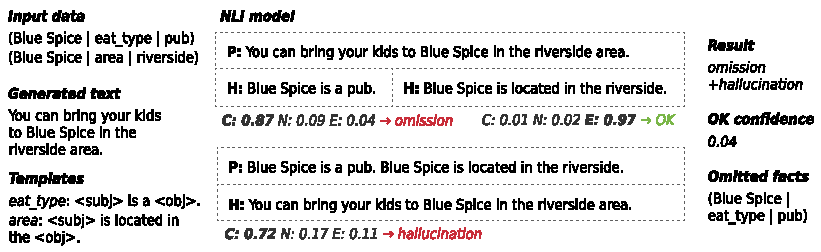
\includegraphics[width=\textwidth]{img/2020_nli_inlg}
    \caption{An example of evaluating the output from a \ac{d2t} system with our metric. The generated text is used as a \textit{premise} (\textit{P}) to check for omissions and as a \textit{hypothesis} (\textit{H}) to check for hallucinations. The \ac{nli} model generates probabilities for \textit{contradiction} (\textit{C}), \textit{neutral} (\textit{N}) and \textit{entailment} (\textit{E}).}
    \label{fig:sem-acc:ex}
\end{figure*}

\paragraph{Checking Semantic Accuracy with NLI} We can use an \ac{nli} model for assessing semantic accuracy of generated texts. Consider the two input facts from \autoref{fig:sem-acc:ex}: $F= $\{\emph{``Blue spice is a pub''}, \emph{``Blue Spice is located in the riverside''}\} and the generated text: $Y= $\emph{``You can bring your kids to Blue Spice in the riverside area.''} We propose using an \ac{nli} model for checking if the semantic information implied by $F$ and $Y$ is equal.
In this case, the model should detect that the first fact is not entailed by the text (there is no mention of Blue Spice being a pub), but the text is also not entailed by the facts (the information about kids is hallucinated).

We achieve this by using the \ac{nli} model to check for entailment in two directions:
\begin{enumerate}
    \item To check for \textrm{omissions}, we use the whole generated text as a premise and sequentially feed each fact as a hypothesis to the \ac{nli} model. Any failed \ac{nli} check is considered an omission.
    \item To check for \textrm{hallucinations}, we concatenate all facts as a premise and feed the generated text as a hypothesis to the \ac{nli} model. If this \ac{nli} check fails, the text is considered to contain hallucination. This step cannot be split into simpler \ac{nli} checks.
\end{enumerate}

The final output of our metric is either 4-way (denoted as \textsc{Fine}) or 2-way (denoted as \textsc{Rough}):
\begin{itemize}
    \item \textsc{Fine}: We output the probabilities of 4 categories: \emph{OK} (i.e., all \ac{nli} checks passed), \emph{omission}, \emph{hallucination}, or \emph{omission+hallucination} (based on the failed checks). The 4-way output is more useful for system evaluation since we can distinguish whether the system tends to hallucinate or omit information.
    \item  \textsc{Rough}: The three failure modes are combined into \emph{not\_OK}. The 2-way output corresponds more to usage inside an \ac{d2t} generation system for output reranking or filtering, where any incorrect should be penalized or filtered out.
\end{itemize}

Additionally, we compute a \textit{confidence score} of the model as the minimum of all the entailment probabilities.


\subsection{Experiments}
\label{sec:sem-acc:experiments}
For our \ac{nli} model, we use the \texttt{roberta-large-mnli}\footnote{\scalebox{0.95}[1.0]{\url{https://huggingface.co/roberta-large-mnli}}} checkpoint of the pretrained RoBERTa model \cite{liuRoBERTaRobustlyOptimized2019}, which was finetuned on the Multi\ac{nli} dataset \cite{williams2018mnli}. We use the model \textit{as is}, without any further training on domain-specific data.
Given a premise text and a hypothesis text, the \ac{nli} model produces a probability distribution over three results: \textit{contradiction}, \textit{neutral},
and \textit{entailment} (see \autoref{sec:sem-acc:method}). We consider a \ac{nli} check as passed if the probability for \textit{entailment} is the highest of the three.


We experiment with the WebNLG and E2E datasets (see \autoref{sec:datasets} for the descriptions of the datasets). Since both datasets were used in shared tasks, we can compare the outputs of our system with the respective measures of semantic accuracy:
\begin{itemize}
    \item For WebNLG, we compare our metric with crowdsourced human ratings of semantic adequacy \cite{shimorinaWebNLGChallengeHuman2019}. In particular, we use the question: \textit{``Does the text correctly represent the meaning in the data?''}, where the human annotators used a three-point Likert scale (1 = Incorrect, 2 = Medium, 3 = Correct). The answers are averaged over multiple annotators. In our experiments, we consider a sentence correct if it achieved a human rating 2.5 or higher.\footnote{We also tried a threshold of 2.0, with slightly worse results.}
    \item For E2E, we compare our metric to the results of the handcrafted automatic script which was used in the E2E challenge \cite{dusekEvaluatingStateoftheartEndtoEnd2020}.\footnote{While the E2E challenge did include crowdsourced evaluation of semantic accuracy, the results were unreliable, overestimating the number of errors \cite{dusekEvaluatingStateoftheartEndtoEnd2020}.} We further use small sets of system outputs and human-written texts with expert annotation \citep[provided by][]{dusekSemanticNoiseMatters2019} to evaluate our approach against gold-standard annotation and to compare to existing semantic accuracy classifiers for E2E data.
\end{itemize}


We evaluate the \emph{Default} and \emph{Backoff} approaches to acquiring templates as described in \autoref{sec:sem-acc:method}. For WebNLG, we obtained templates by delexicalizing human references for single-triple examples from WebNLG training data.\footnote{For each predicate, we choose randomly if more templates are found and use the backoff if no templates are found.} For E2E, we handcrafted eight templates for each predicate in the dataset.

\subsection{Evaluation}
\label{sec:sem-acc:evaluation}

\begin{table}[t]
    \centering \small
    \begin{tabular}{l ccccc>{\hspace{3mm}}ccccc} \toprule
                & \multicolumn{5}{c}{\bfseries WebNLG} & \multicolumn{5}{c}{\bfseries E2E}                                                                                                                  \\
                & \textbf{A}                           & \textbf{R}                        & \textbf{P} & \textbf{F1} & $\mathbf{\rho}$ & \textbf{Af} & \textbf{Ar} & \textbf{R} & \textbf{P} & \textbf{F1} \\\midrule
        Default & 0.775                                & 0.772                             & 0.796      & 0.784       & 0.628           & 0.911       & 0.933       & 0.895      & 0.910      & 0.903       \\
        Backoff & 0.768                                & 0.760                             & 0.793      & 0.776       & 0.637           & 0.846       & 0.874       & 0.913      & 0.768      & 0.834       \\ \bottomrule
    \end{tabular}
    \caption{WebNLG and E2E results, compared to crowdsourced human ratings and the automatic evaluation script, respectively (A = accuracy, Af = \textsc{Fine} accuracy, Ar = \textsc{Rough} accuracy, R = recall, P = precision, F1 = F-measure, $\rho$ = Spearman correlation of confidence scores with human scores).}
    \label{tab:sem-acc:res}
\end{table}



We evaluate our metric in terms of accuracy, precision, recall, and F1-measure (where \emph{not\_OK} samples are treated as positive since we focus on detecting errors). The overall scores for both datasets are summarized in \autoref{tab:sem-acc:res}.
We additionally perform a manual error analysis on a random sample of 100 error examples for each dataset, i.e., examples where our metric gave a different assessment from the ground truth.


% The results for the E2E dataset are better, probably due to the lower lexical variability of the dataset.
% \OD{a možná kvůli tomu, že human eval pro webnlg je trochu zašuměný, ale nevim, jestli se to sem hodí}


% recall is probably more important than precision (not that there are differences)

\paragraph{WebNLG Analysis} The Spearman correlation of our model's confidence scores with the average human scores on the WebNLG dataset is moderate (around 63\%; $p<$1e-10). Our manual error analysis indicates several potential sources of discrepancies:
\begin{enumerate}
    \item The human annotation is somewhat noisy---many correctly rendered outputs do not reach the 2.5 threshold, while some incorrect ones do.
    \item The human annotators also tend to give lower scores to accurate but ungrammatical or poorly organized texts, while our metric tends to rate these texts as \emph{OK}.
    \item Imprecise templates can confuse the \ac{nli} (e.g., for the predicate \emph{nationality}, our extracted template is \emph{\textless{}subj\textgreater{} was \textless{}obj\textgreater{}}, which works well with values such as \emph{French}, but not with \emph{United States}). This is a weak point of our metric, as illustrated by the very small performance difference between the \emph{Default} and \emph{Backoff} setups. However, the issue can be mitigated by a better selection of the templates from training data, e.g., using language-model scoring.
\end{enumerate}

Moreover, our re-examination shows that almost half of the error examples (42 out of 100) were in fact correctly classified by our metric (i.e., their crowdsourced human annotation was incorrect),  so the true performance is most likely higher than the reported numbers.

%  This is similar to $n$-gram-based metrics on this data (\citealp{shimorinaWebNLGChallengeHuman2019} reports 0.59 for \acs{bleu} and 0.73 for METEOR), but unlike these metrics, our approach does not require human-written reference texts.

% To further check whether the size of the input affects performance, we computed Spearman correlation of the number of input triples with metric errors. The resulting very low value of -0.05 ($p=$\,0.02, \emph{Default} setting) shows that the metric holds its performance even for more complex WebNLG examples.
%
% On the other hand, heck for different information 


%Third, we note that many examples are dubious, e.g. there are typos in the text or the text interprets the data too loosely. In these cases, the notion of semantic accuracy can differ between the annotators.





\paragraph{E2E Analysis} The results for the E2E dataset are very good compared to the WebNLG dataset, with over 90\% agreement with the handcrafted script. This can be attributed to lower lexical variability and less noisy texts, as well as to the better quality of the handcrafted templates (the difference between the \emph{Default} and \emph{Backoff} setups is much more pronounced here). The main issues identified by our error analysis are:
\begin{enumerate}
    \item Problems in the interpretation of some values, e.g., \textit{price range=less than \textsterling{}20} is verbalized as ``cheap'' or \textit{family-friendly=no} as ``adult-only''. These cases are classified as \emph{not\_OK} by the \ac{nli} model.
    \item Missing or over-greedy patterns in the slot error script, causing annotation errors.
    \item Edge cases: some expressions cannot be interpreted in a straightforward way, e.g., ``high restaurant'' for \emph{pricerange=high} is deemed OK by the \ac{nli} but not by the slot error script.
    \item Expressions in the outputs that do not correspond to input facts, such as ``with full service'', are considered hallucinations by the \ac{nli} but ignored by the slot error script.
\end{enumerate}
Again, we consider about half of the error examples (45 out of 100) as correctly classified by our metric, and thus our metric's performance is probably higher than the reported values.

\subsection{Discussion}

\paragraph{Comparison to Other Metrics} The main alternatives to our metric are mostly reference-based, which makes their use-cases different from ours \cite{zhaoMoverScoreTextGeneration2019,sellam2020bleurt,yuanBARTScoreEvaluatingGenerated2021}. Except for PARENT \cite{dhingraHandlingDivergentReference2019} and RoMe \cite{ronyRoMeRobustMetric2022}, these metrics are not targetting \ac{d2t} generation. Our metric thus remains a major alternative for evaluating the semantic accuracy of data-to-text generation, especially with \ac{rdf} triples on the input. In the future, a more flexible metric for evaluating semantic accuracy can be potentially based on large language models \cite{zhaoInvestigatingTabletoTextGeneration2023,sottanaEvaluationMetricsEra2023,kocmiLargeLanguageModels2023}, a topic to which we return in \autoref{sec:quintd}.

\paragraph{Limitations} Perhaps surprisingly, the main bottleneck of the metric is not in the capabilities in \ac{nli} model. Although the \ac{nli} model is not perfect, \citet{chenMENLIRobustEvaluation2022} have shown that out-of-the-box \ac{nli} models are generally better and more robust metrics than specially trained approaches. In many cases, however, converting the structured data to a format suitable to \ac{plm} can be non-trivial. In this respect, see the discussion on automating template generation with \acp{plm} and \acp{llm} in \autoref{sec:pipeline:discussion}.


\section{Token-Level Error Classification}
\label{sec:tok-eval}

\begin{refbox}
    This section is based on the paper \emph{Text-in-Context: Token-Level Error Detection for Table-to-Text Generation} \cite{kasnerTextinContextTokenLevelError2021}, joint work with Simon Mille and Ondřej Dušek, published in the Proceedings of the 14th International Conference on Natural Language Generation (INLG 2021). The work describes our submission to the Shared Task on Evaluating Accuracy in Generated Texts. The project was led by the author of the thesis; Simon Mille provided the rule-based generator and wrote its description.
\end{refbox}


In this section, we present an automatic metric for \ac{d2t} generation that can detect semantic accuracy errors in the generated text on the \emph{token level}. Our metric combines a rule-based \ac{d2t} generation system and \acp{plm}. We first use a rule-based \ac{d2t} generation system to generate all the facts that can be derived from the input. For each sentence we evaluate, we select a subset of relevant facts by measuring their semantic similarity with the examined sentence. For annotating erroneous tokens, we finetune a pretrained language model for token-level classification, using the annotated data with the relevant facts in the context as the ground truth.

On the test set of the Shared Task on Evaluating Accuracy in Generated Texts \cite{thomsonGenerationChallengesResults2021}, we achieve 69\% recall and 75\% precision with a model trained on a mixture of human-annotated and synthetic data, placing first out of four submissions in the track for automatic metrics. The code for our experiments is available on Github.\footnote{\url{https://github.com/kasnerz/accuracySharedTask_CUNI-UPF}}


\subsection{Motivation}
\label{sec:tok-acc:motivation}


In \autoref{sec:sem-acc}, we presented a metric for detecting semantic errors for \ac{d2t} generation at the level of individual data items. The metric is well-suited for cases where the text should mention \emph{all the data on the input}, as it can report individual missing items (omissions). However, it is less suitable for detecting incorrect information in the text (hallucinations), as it can give only a single ``hallucination score'' for the entire text. This is problematic for the texts generated from complex data, where the omissions are not relevant (since we do not verbalize all the input data), but the system can still produce numerous hallucinations.


An example of a dataset with complex data is Rotowire (\citealp{wiseman2017challenges}; see \autoref{sec:datasets} for details). In this dataset, the task is to generate basketball match summaries from tabular data. Rotowire poses multiple challenges for neural systems, including the fact that it requires content selection or that its human-written training texts are themselves not always grounded in data, which makes neural models more susceptible to hallucination.
The output texts are also usually longer, which makes the hallucinations more common and detecting hallucination errors on a more fine-grained level essential.

There is, however, no established way to check for hallucinations automatically. Specific content-checking metrics mostly remain a domain of handcrafted pattern matching \cite{wen2015semantically,dusekSemanticNoiseMatters2019}, which does not scale well to new domains. While human evaluation provides a more reliable alternative, it is costly and difficult to set up \cite{van2019best,belzDisentanglingPropertiesHuman2020,thomsonGoldStandardMethodology2020}. Regarding neural metrics such as BERTScore \cite{zhang2019bertscore} or BLEURT \cite{sellam2020bleurt}, most of them have not been evaluated for content preservation, especially on the level of individual tokens.


\subsection{Shared Task in Evaluating Accuracy}
\label{sec:tok-acc:st}
The goal of the Shared Task on Evaluating Accuracy in Generated Texts at INLG 2021 was to develop a token-level error annotation metric for complex \ac{d2t} generation \cite{reiterSharedTaskEvaluating2020}. The organizers of the shared task first manually annotated 60 outputs of various neural systems trained on Rotowire, using the error types defined in \citet{thomsonGoldStandardMethodology2020}:
\begin{itemize}
    \item \errnum{NUMBER} --  Incorrect number (both digits and numerals).
    \item \errent{NAME} -- Incorrect named entity (people, places, teams, days of the week).
    \item \errword{WORD} -- Incorrect word which is not one of the above.
    \item \errctx{CONTEXT} --  A phrase inappropriate for the context.
    \item \errnc{NOT\_CHECKABLE} --  A statement which cannot be checked.
    \item \errother{OTHER} --  Any other type of mistake.
\end{itemize}
\begin{figure}[t]
    \footnotesize
    \lineacross{}


    The Memphis Grizzlies (5-\errnum{2}) defeated the Phoenix Suns (3 - 2) \errent{Monday} 102-91 at the \errent{Talking Stick Resort Arena} in Phoenix. The Grizzlies had a \errword{strong} first half where they \errword{out-scored} the Suns \errnum{59}-\errnum{42}. Marc Gasol scored 18 points, \errword{leading} the Grizzlies.  \errctx{Isaiah Thomas added} 15 points, he is \errnc{averaging 19 points on the season so far}.
    \vspace{1mm}

    \begin{itemize}
        \item \errnum{2}                                       -- Incorrect number, should be 0.
        \item \errent{Monday}                                  -- Incorrect named entity, should be Wednesday.
        \item \errent{Talking Stick Resort Arena}              -- Incorrect named entity, should be US Airways Center.
        \item \errword{strong}                                 -- Incorrect word, the Grizzlies did not do well in the first half.
        \item \errword{out-scored}                             -- Incorrect word, the Suns had a higher score in first half.
        \item \errnum{59}                                      -- Incorrect number, should be 46.
        \item \errnum{42}                                      -- Incorrect number, should be 52 .
        \item \errword{leading}                                -- Incorrect word.  Marc Gasol did not lead the Grizzlies, Mike Conley did with 24 points.
        \item \errctx{Isaiah Thomas added}                     -- Context error.  Thomas played for the Suns, but context here implies he played for the Grizzlies and added to their score.
        \item \errnc{averaging 10 points on the season so far} -- Not checkable.  This is very hard to check, since data sources report performance per season and per game, not performance up to a particular point in a season.
    \end{itemize}
    \lineacross{}

    \caption{Example text with error annotations adapted from \citet{thomsonGenerationChallengesResults2021}, using the error marking style from \citet{thomsonEvaluatingFactualAccuracy2023}. The original data for this game is available at \url{https://www.basketball-reference.com/boxscores/201411050PHO.html} .}
    \label{fig:tok-eval:example}
\end{figure}
An example of an annotated system output is provided in \autoref{fig:tok-eval:example}. The objective of the shared task was to either implement an automatic metric for creating the same type of annotations automatically or to develop a human evaluation scenario capable of producing the same annotations while requiring fewer resources.


% Our submission for the shared task falls into the first category:
% we developed an automatic metric for token-level error annotation which combines a rule-based generation system with a neural retrieval model and a pretrained neural LM used for error tagging.
% We evaluated our approach in a cross-validation scenario to select the best configuration for the shared task. Overall, our system is able to reach 65\% error detection F1 score and ranked first out of four automatic submissions in the shared task.



\subsection{Our System}
\label{sec:tok-eval:system}

\begin{figure*}[ht]
    \centering
    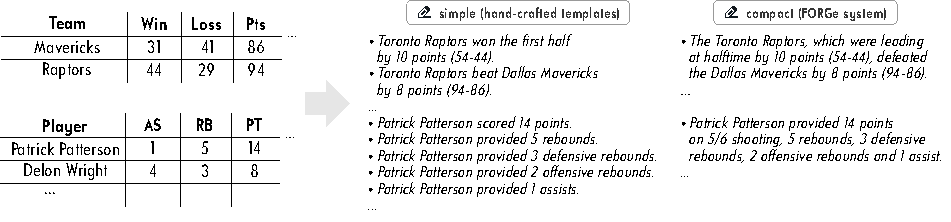
\includegraphics[width=\textwidth]{img/tok-eval_generator.pdf}
    \caption{Rule-based NLG which we use to generate facts from the input data. The facts are used as an input to the error checking model (see Figure \ref{fig:tok-eval:system}). We experiment with (a) simple hand-crafted templates and (b) compact sentences generated by the FORGe system.}
    \label{fig:tok-eval:gen}
\end{figure*}





Our submission for the shared task falls into the first category: we developed an automatic metric based on a \ac{plm}, which marks each token in the output text for the presence of errors. To make the tabular data understandable for the \ac{plm}, we use a rule-based system to exhaustively generate all the facts that can be derived from the data. Since the context window of the \ac{lm} is limited, we also use a neural-based retrieval system to retrieve only $c$ relevant facts, which are added into the context window of the \ac{lm} to support its decisions. We describe individual components of our system below.

% We developed an automatic metric for token-level error annotation which combines (1) a rule-based sentence generation system, (2) a neural retrieval model, and (3) a pretrained encoder \ac{lm} used for error tagging. The idea behind our system is that the pretrained encoder will compare the output with the relevant context retrieved from the data, tagging errors on the token level.

% Our system is composed of three steps, which we describe below:
% \begin{enumerate}
% \item A rule-based generator for fact descriptions,
% \item A retrieval system for selecting facts relevant for a given sentence,
% \item A token-level error tagger.
% \end{enumerate}


\paragraph{Rule-based Fact Descriptions}
We use a rule-based system to generate facts from the input tables in natural language. For each game, we generate facts about the game (hosting team, visiting team, date converted to weekday), line-score objects (team name and statistics), and box-score objects (player name, player team, player starting position and their personal statistics). We also generate additional facts that can be inferred from the input table, such as which team won and by how much, comparisons between the team and player raw data (e.g., \emph{Team A and Team B committed the same number of fouls}), details based on statistics (e.g., \emph{Player X recorded a double-double}), or an interpretation of some numbers (e.g., \emph{Team A came back in the 4th quarter}).\footnote{A number of facts frequently mentioned in human-written descriptions could not be obtained from the Rotowire data, as for instance the player stats per quarter, a career-high points total, whether a player is an all-star or not, or if a player scored the winning shot.}

We experiment with both \emph{simple} descriptions created by filling in sentence templates and \emph{compact} descriptions generated using a grammar-based system:
\begin{itemize}
    \item \textbf{Simple descriptions} are produced by a template-based system, with one template per fact. We handcrafted 129 sentence templates to cover all the facts described above. A sentence template looks like the following: ``\textit{[PLAYER$\_$NAME] scored [PTS] points.}'', where square brackets indicate variables that are instantiated with the corresponding input values (see Figure~\ref{fig:tok-eval:gen} for sample sentences).
    \item  \textbf{Compact descriptions} are produced by the FORGe system \cite{mille2019teaching}, which allows for the generation of more compact sentences.  For instance, the five bottom sentences from the simple system in \autoref{fig:tok-eval:gen} are covered by the single bottom sentence from the compact system. FORGe performs surface realization in several steps, by first aggregating the templates based on the predicate and argument identity and then structuring, linearizing, and inflecting components of the sentences. The FORGe grammars were used off-the-shelf,\footnote{We deactivated cross-sentence referring expression generation so that each generated sentence can be used independently.} with additional 98 manually crafted abstract templates.
\end{itemize}

The simple system produces about 569 facts for each game. The compact system covers the same amount of information with more syntactically complex sentences, producing about 112 sentences per game, i.e., five times less.


\begin{figure*}[t]
    \centering
    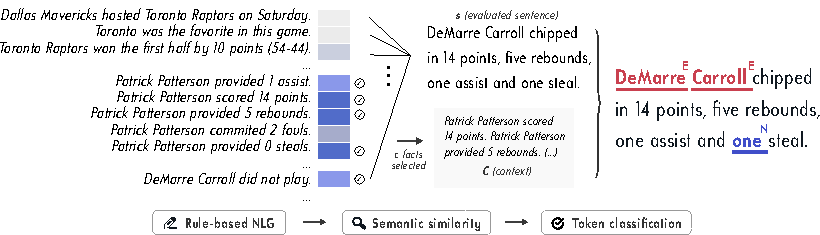
\includegraphics[width=\textwidth]{img/tok-eval_system.pdf}
    \caption{An overview of our system. First, we generate the facts from the input table with a rule-based NLG system (see Figure \ref{fig:tok-eval:system}). For each evaluated sentence $s$, we select $c$ facts with the highest semantic similarity, getting a context $C$. The pair $(C, s)$ is given as an input to a pretrained LM for token-level error classification.}
    \label{fig:tok-eval:system}
\end{figure*}

\paragraph{Context Retrieval} The maximum length of the input sequence for our error tagger is 512 tokens, which is about 10\% of the total length of the generated sentences $G$. Therefore, we select only a subset of $G$, which we refer to as \emph{context} $C$. For each generated sentence $g_i\in G$, we measure semantic similarity between $g_i$ and the evaluated sentence $s$ using Sentence Transformers \cite{reimers-gurevych-2019-sentence}. In particular, we embed the sentence tokens by applying mean pooling on the output of \texttt{paraphrase-distilroberta-base-v2}, getting the embedding vectors $e_{s}$ and $e_{g_i}$. Then, we compute the cosine similarity between the embeddings:
\begin{align}
    score = \frac{e_s \cdot e_{g_i}}{\lVert e_s \rVert \lVert e_{g_i} \rVert}.
\end{align}
For the context $C$, we select the top $c$ sentences from $G$ that have the highest cosine similarity to $s$.


\paragraph{LM-based Error Tagger}
As our error tagger, we use RoBERTa \cite{liuRoBERTaRobustlyOptimized2019} with a token-level classification head. The model receives an input $X = (C, s)$ and is trained to annotate each token in $s$ either with an \textit{OK} label or with a label corresponding to one of the error categories. We experiment with two data sources for training the model:
\begin{itemize}
    \item \emph{gold-standard annotated data} from the shared task (which contains all error types),
    \item \emph{synthetic data} created by perturbing the human-written summaries from Rotowire (which contains only \errent{NAME} and \errnum{NUMBER} errors).
\end{itemize}
% For our submission, we use two-stage finetuning: first we finetune on synthetic data, then we finetune on the annotated data. 
% \ODdel{A cross-validation on the development set gives us 65\% F1-score (61\% precision and 69\% recall).}\OD{I'd include at least bits of the mega-table instead.}

\paragraph{Synthetic Data} The gold-standard data contains only 60 games, as opposed to 3,395 games in the Rotowire training set. This led us to the idea of using the training set as a source of synthetic data, introducing errors into human-written descriptions. We focus only on the \errent{NAME} and \errnum{NUMBER} errors, i.e., the categories that are the most represented and also easiest to generate. In each sentence, we identify named entities in the text using \emph{spaCy}.\footnote{\url{https://spacy.io}} We modify only a certain portion of entities according to the \emph{entity modification rate} (EMR), which we treat as a hyperparameter. We introduce the \errent{NAME} errors by:
\begin{enumerate}
    \item swapping the names of teams with opponent teams,
    \item swapping the names of players with other players in the game,
    \item swapping the names of cities with other cities in the Rotowire dataset,
    \item modifying the days of the week.
\end{enumerate}
For \errnum{NUMBER} errors, we take an integer $n$ identified in the text, sample a number from a normal distribution with $\mu=n$ and $\sigma=3$, and truncate it to get an integer. We re-sample if the output equals the original number or for negative outputs. If the number is spelled out, we use \texttt{text2num}\footnote{\url{https://pypi.org/project/text2num/}} and  \texttt{num2words}\footnote{\url{https://pypi.org/project/num2words/}} to convert to digits and back.


\subsection{Experiments}
\label{sec:tok-eval:experiments}

We train a PyTorch version of RoBERTa from the Huggingface Transfomers repository \cite{wolf2019HuggingFacesTS} using the AdamW optimizer \cite{loshchilov2018fixing}, learning rate $5\times10^{-5}$ and linear warmup.
% $\beta_1=0.9, \beta_2=0.997, \epsilon=10^{-8}$, 
We finetune the model for 10 epochs and select the model with the highest validation score.
We experiment with several hyperparameters: % regarding our training data: 
\begin{itemize}
    \item \emph{simple} vs.~\emph{compact} sentences in $G$, % (Section \ref{sec:rule-based-system})
    \item  \textit{number of sentences} retrieved for the context: $c$ = 5, 10, 20 or 40;
    \item \textit{entity modification rate} (EMR): proportion of entities modified in the synthetic data: 0.25, 0.5, or 0.75.
\end{itemize}
We evaluate the model using a script provided by the organizers, which computes recall and precision of the model output with respect to the human-annotated data. Since we use the human-annotated data for training, we perform 6-fold cross-validation: in each run, we use 45 games for training, 5 games for validation, and 10 games for evaluation.


\begin{table*}[!htbp]
    \centering\footnotesize
    \begin{tabular}{@{}l l r >{\hspace{2mm}} ccc >{\hspace{2mm}} ccc >{\hspace{2mm}} ccc@{}}\toprule
        \multirow{2}{*}{\bf Gen.}                    & \multirow{2}{*}{\bf Data} & \multirow{2}{*}{$c$} & \multicolumn{3}{c}{\bf EMR = 0.25} & \multicolumn{3}{c}{\bf EMR = 0.5} & \multicolumn{3}{c}{\bf EMR = 0.75}                                                         \\
                                                     &                           &                      & R                                  & P                                 & F1                                 & R         & P     & F1    & R         & P     & F1    \\\midrule
        \multirow{8}{*}{\bf\rotatebox{90}{Simple} }  & \multirow{4}{*}{s}
                                                     & 5                         & 0.123                & 0.723                              & 0.210                             & 0.165                              & 0.512     & 0.250 & 0.310 & 0.323     & 0.316         \\
                                                     &                           & 10                   & 0.138                              & 0.737                             & 0.232                              & 0.181     & 0.549 & 0.272 & 0.328     & 0.400 & 0.360 \\
                                                     &                           & 20                   & 0.137                              & \bf 0.741                         & 0.231                              & 0.179     & 0.559 & 0.271 & 0.327     & 0.433 & 0.373 \\
                                                     &                           & 40                   & 0.165                              & 0.712                             & 0.268                              & 0.199     & 0.560 & 0.294 & 0.296     & 0.436 & 0.353 \\\cdashlinelr{2-12}
                                                     & \multirow{4}{*}{s+h}
                                                     & 5                         & 0.422                & 0.617                              & 0.501                             & 0.414                              & 0.594     & 0.488 & 0.401 & 0.583     & 0.475         \\
                                                     &                           & 10                   & 0.467                              & 0.551                             & 0.506                              & 0.438     & 0.638 & 0.519 & 0.428     & 0.665 & 0.521 \\
                                                     &                           & 20                   & 0.518                              & 0.640                             & 0.573                              & 0.544     & 0.575 & 0.559 & 0.509     & 0.595 & 0.549 \\
                                                     &                           & 40                   & 0.584                              & 0.644                             & \bf 0.613                          & \bf 0.595 & 0.612 & 0.603 & 0.519     & 0.639 & 0.573 \\\midrule
        \multirow{8}{*}{\bf \rotatebox{90}{Compact}} & \multirow{4}{*}{s}
                                                     & 5                         & 0.151                & \bf 0.696                          & 0.248                             & 0.170                              & 0.617     & 0.267 & 0.336 & 0.427     & 0.376         \\
                                                     &                           & 10                   & 0.176                              & 0.663                             & 0.278                              & 0.195     & 0.624 & 0.297 & 0.295     & 0.486 & 0.367 \\
                                                     &                           & 20                   & 0.196                              & 0.672                             & 0.303                              & 0.205     & 0.635 & 0.310 & 0.278     & 0.552 & 0.370 \\
                                                     &                           & 40                   & 0.166                              & 0.643                             & 0.264                              & 0.197     & 0.595 & 0.296 & 0.306     & 0.530 & 0.388 \\ \cdashlinelr{2-12}
                                                     & \multirow{4}{*}{s+h}
                                                     & 5                         & 0.600                & 0.641                              & 0.620                             & 0.552                              & 0.635     & 0.591 & 0.588 & 0.600     & 0.594         \\
                                                     &                           & 10                   & 0.583                              & 0.662                             & 0.620                              & 0.629     & 0.606 & 0.617 & \bf 0.656 & 0.606 & 0.630 \\
                                                     &                           & 20                   & 0.622                              & 0.647                             & 0.634                              & 0.597     & 0.688 & 0.639 & 0.600     & 0.660 & 0.629 \\
                                                     &                           & 40                   & 0.614                              & 0.690                             & \bf \phantom{*}0.650*              & 0.609     & 0.630 & 0.619 & 0.611     & 0.630 & 0.620 \\\bottomrule
    \end{tabular}
    \caption{Recall (R), precision (P) and F1 scores on development data. $s$ stands for synthetic training data and $h$ for human training data.  $c$ indicates the number of sentences in the context provided to the tagger, EMR stands for entity modification rate. Best recall, precision and F1 scores for both generators (simple and compact) are shown in bold, the submitted model is identified by an asterisk (*).}
    \label{tab:tok-eval:results}
\end{table*}

\paragraph{Development Results} The results of our model on the development data are listed in Table \ref{tab:tok-eval:results}.\footnote{Due to space constraints, we do not list the results of model trained only on annotated data. The results were overall in the 0.3-0.5 range for both recall and precision, and no model was the best-performing one in terms of any metric.} For our final submission, we selected the model with the best F1-score overall, which is 0.65 (61\% recall and 69\% precision). The model uses 40 compact sentences in context, 0.25 EMR, and was trained on both synthetic and human-annotated data. Although compact texts are generally helpful, there are also some well-performing models using simple templates only. A higher number of sentences in context may help to achieve better F1-score, but not always (the longer context is also sometimes cropped to fit the input). Using a higher EMR then generally leads to higher recall, suggesting that the model adapts to the base rate of errors.

\begin{table}[t]
    \centering\small
    \begin{tabular}{l cccc}\toprule
        \multirow{2}{*}{\bf Error Type} & \multicolumn{2}{c}{\bf Mistake} & \multicolumn{2}{c}{\bf Token}                 \\
                                        & R                               & P                             & R     & P     \\ \midrule
        \errent{NAME}                   & 0.750                           & 0.846                         & 0.759 & 0.862 \\
        \errnum{NUMBER}                 & 0.777                           & 0.750                         & 0.759 & 0.752 \\
        \errword{WORD}                  & 0.514                           & 0.483                         & 0.465 & 0.529 \\
        \errctx{CONTEXT}                & 0.000                           & -                             & 0.000 & -     \\
        \errnc{NOT\_CHECKABLE}          & 0.000                           & -                             & 0.000 & -     \\
        \errother{OTHER}                & 0.000                           & -                             & 0.000 & -     \\ \noalign{\vskip 0.1cm}\hdashline\noalign{\vskip 0.1cm}
        \textbf{Overall}                & 0.691                           & 0.756                         & 0.550 & 0.769 \\\bottomrule
    \end{tabular}
    \caption{Results of our system on test data: recall (R) and precision (P) are shown for individual error types.}
    \label{tab:tok-eval:results-test}
\end{table}

\paragraph{Submission Results}
Table \ref{tab:tok-eval:results-test} shows the results of our model on the official test data of the task, broken down by error types. The overall scores are higher than on the development set -- test set recall is 0.691 (vs.~0.614 on the development set), and precision is 0.756 (vs.~0.690). The fact that we used all the available human-annotated data for training the final model may have contributed to the difference, but it is also possible that the test data was somewhat less challenging. We note that our model was able to identify only three types of errors (\errent{NAME}, \errnum{NUMBER}, \errword{WORD}), having better results for the \errent{NAME} and \errnum{NUMBER} errors. We believe the explanation is two-fold: the names and numbers are often found verbatim in the input data (and in our generated facts), which makes them easy to detect, and also the corresponding error types were the most represented in the training data. In contrast, the three error types that were not detected are much less represented in the training data and hard to detect in our setup.


\subsection{Discussion}
\paragraph{Limitations} Our metric depends on the existence of a rule-based system for generating factual statements from the data. Such a system may be hard to develop, even though we have shown that simple templates can be similarly efficient as more complex approaches. As our approach is data-driven, it also requires the system outputs annotated with errors. This requirement may be partially mitigated by using synthetic data. In our case, using synthetic data only results in low recall (see \autoref{tab:tok-eval:results}), but more sophisticated techniques for creating the synthetic data lead to better results.

\paragraph{How to Improve The Metric} Our submission achieved the best results in the automatic metrics category, but there is still a gap with what humans can achieve, as shown by the Laval University submission's overall 0.841 recall and 0.879 precision \cite{garneau2021laval}. One way to improve our system would be to enrich the reference fact descriptions by either inferring more information from the raw data or by extracting additional data from external databases. Another option would be to add surrounding sentences to the context -- this could help to resolve coreferences (e.g., if a player is referred to as \textit{"He"}) and to detect the \errctx{CONTEXT} errors.

\paragraph{LLM-based Alternatives} Recently, the evaluation metrics based on \acp{llm} are starting to provide an alternative, more flexible approach for evaluating generated texts \cite{zhaoInvestigatingTabletoTextGeneration2023,sottanaEvaluationMetricsEra2023,chiang-lee-2023-large,fu2023gptscore}. An advantage of the \ac{llm}-based metrics is the possibility of defining custom error categories without the need for having annotated data for finetuning the model. We explore such an approach in \autoref{sec:quintd}, where we use a \ac{llm}-based metric for token-level evaluation of generated text. However, it should be noted that with \ac{llm}-based metrics, greater flexibility is traded for lower controllability (especially in the case of closed-source models), making the evaluation potentially biased and hard to reproduce \cite{stureborgLargeLanguageModels2024,kooBenchmarkingCognitiveBiases2023,wangLargeLanguageModels2023}.

\section{Conclusion}
We introduced two metrics for evaluating the semantic accuracy of \ac{d2t} generation. The metric presented in \autoref{sec:sem-acc} targets the cases where all the data items need to be mentioned in the output text. The metric uses a combination of simple templates and an off-the-shelf neural model, making our approach applicable with minimal additional effort. The metric introduced in \autoref{sec:tok-eval} then targets complex data-to-text generation, enabling annotating factual errors on the level of individual tokens.

\chapter{Unified Data Processing and Visualization}
\label{chap:tabgenie}

In \autoref{sec:tabgenie}, we make a step towards unified processing of \ac{d2t} generation datasets. We first convert the input data in 16 datasets of various formats and provenance (loosely related through the task of ``generating text based on data'') into a common tabular format. We take advantage of the unified access to the datasets for building \textsc{TabGenie}: a toolkit combining web interface, command-line interface and Python bindings for simplifying data visualization and processing. While data visualization helps us to get uncover contents of individual datasets, unified format opens up a posibility of streamlining datasets into \acp{plm} for multi-task training. Interactive mode, in which the model input can be modified on-the-fly, then helps us to to insights into the system behavior, the topic to which we will return in \autoref{chap:investigating}. In the end of the section, we present multiple real-world use-cases of our framework.


\section{TabGenie Toolkit}
\label{sec:tabgenie}

\begin{refbox}
    This section is based on the paper \emph{\textsc{TabGenie}: A Toolkit for Table-to-Text Generation} \cite{kasnerTabGenieToolkitTabletoText2023}, joint work with Ekaterina Garanina, Ondřej Plátek, and Ondřej Dušek. The work was published as a system demonstration in the Proceedings of the 61st Annual Meeting of the Association for Computational Linguistics (ACL 2023). The project was led by the author of the thesis, the other authors helped with implementing the framework and paper writing.
\end{refbox}


In this section, we present \textsc{TabGenie} -- a toolkit which enables researchers to explore, preprocess, and analyze a variety of \ac{d2t} generation datasets as tables with associated metadata. The web interface of \textsc{TabGenie} provides an interactive mode for debugging table-to-text generation models, facilitates side-by-side comparison of generated system outputs, and allows easy exports for manual analysis. \textsc{TabGenie} is also equipped with command line processing tools and Python bindings for unified dataset loading and processing. We release \textsc{TabGenie} as a Python package\footnote{\url{https://pypi.org/project/tabgenie/}} and provide its open-source code and a live demo through Github.\footnote{\url{https://github.com/kasnerz/tabgenie}}

\subsection{Motivation}
\label{sec:tabgenie:motivation}
In \autoref{tab:datasets}, we provided a representative, although not comprehensive, overview of research datasets for \ac{d2t} generation. As the number of datasets keeps growing and research keeps accelerating, researchers need to streamline their interactions with these datasets. However, each dataset comes with a different input format and task description, and the input data may not be easy to access and visualize.  Platforms such as HuggingFace Datasets \cite{lhoest2021datasets} or the GEM benchmark \cite{gehrmannGEMBenchmarkNatural2021}  provide a unified way to access the datasets, but they platforms still leave the majority of the data processing load on the user.

A key component missing from current \ac{d2t} tools is the possibility to visualize the input data and generated outputs. Visualization plays an important role in examining and evaluating scientific data \cite{Kehrer2013VisualizationAV} and can help researchers to make more informed design choices. A suitable interface can also encourage researchers to step away from unreliable automatic metrics \cite{gehrmannRepairingCrackedFoundation2022} and focus on manual error analysis \cite{van_miltenburg_underreporting_2021,van_miltenburg_barriers_2023}.

Along with that, demands for a \textit{unified input data format} have recently been raised with multi-task training for large language models (LLMs) \citep[\textit{inter alia}]{sanh2021multitask,scao2022bloom,ouyang2022TrainingLM}. Some works have used simple data linearization techniques for converting structured data to a textual format, in order to align it with the format used for other tasks \cite{xieUnifiedSKGUnifyingMultiTasking2022,tang2022mvp}. However, linearizations are using custom preprocessing code, leading to discrepancies between individual works.

To address these gaps, we present \textsc{TabGenie} -- a multi-purpose toolkit for interacting with \ac{d2t} generation datasets. The cornerstone of \textsc{TabGenie} is a \emph{unified data representation}. Each input represented is as a matrix of $m$ columns and $n$ rows consisting of individual cells accompanied with metadata. Building upon this representation, \textsc{TabGenie} then provides multiple features for unified workflows with table-to-text datasets, including:
\begin{enumerate}
    \item visualizing individual dataset examples in the tabular format,
    \item interacting with table-to-text generation systems in real-time,
    \item comparing generated system outputs,
    \item loading and preprocessing data for downstream tasks,
    \item exporting examples and generating spreadsheets for manual error analysis.
\end{enumerate}

\subsection{Data}
\label{sec:tabgenie:data}

\begin{figure*}[t]
    \centering
    \setlength{\fboxsep}{0pt}\fcolorbox{gray!20}{white}{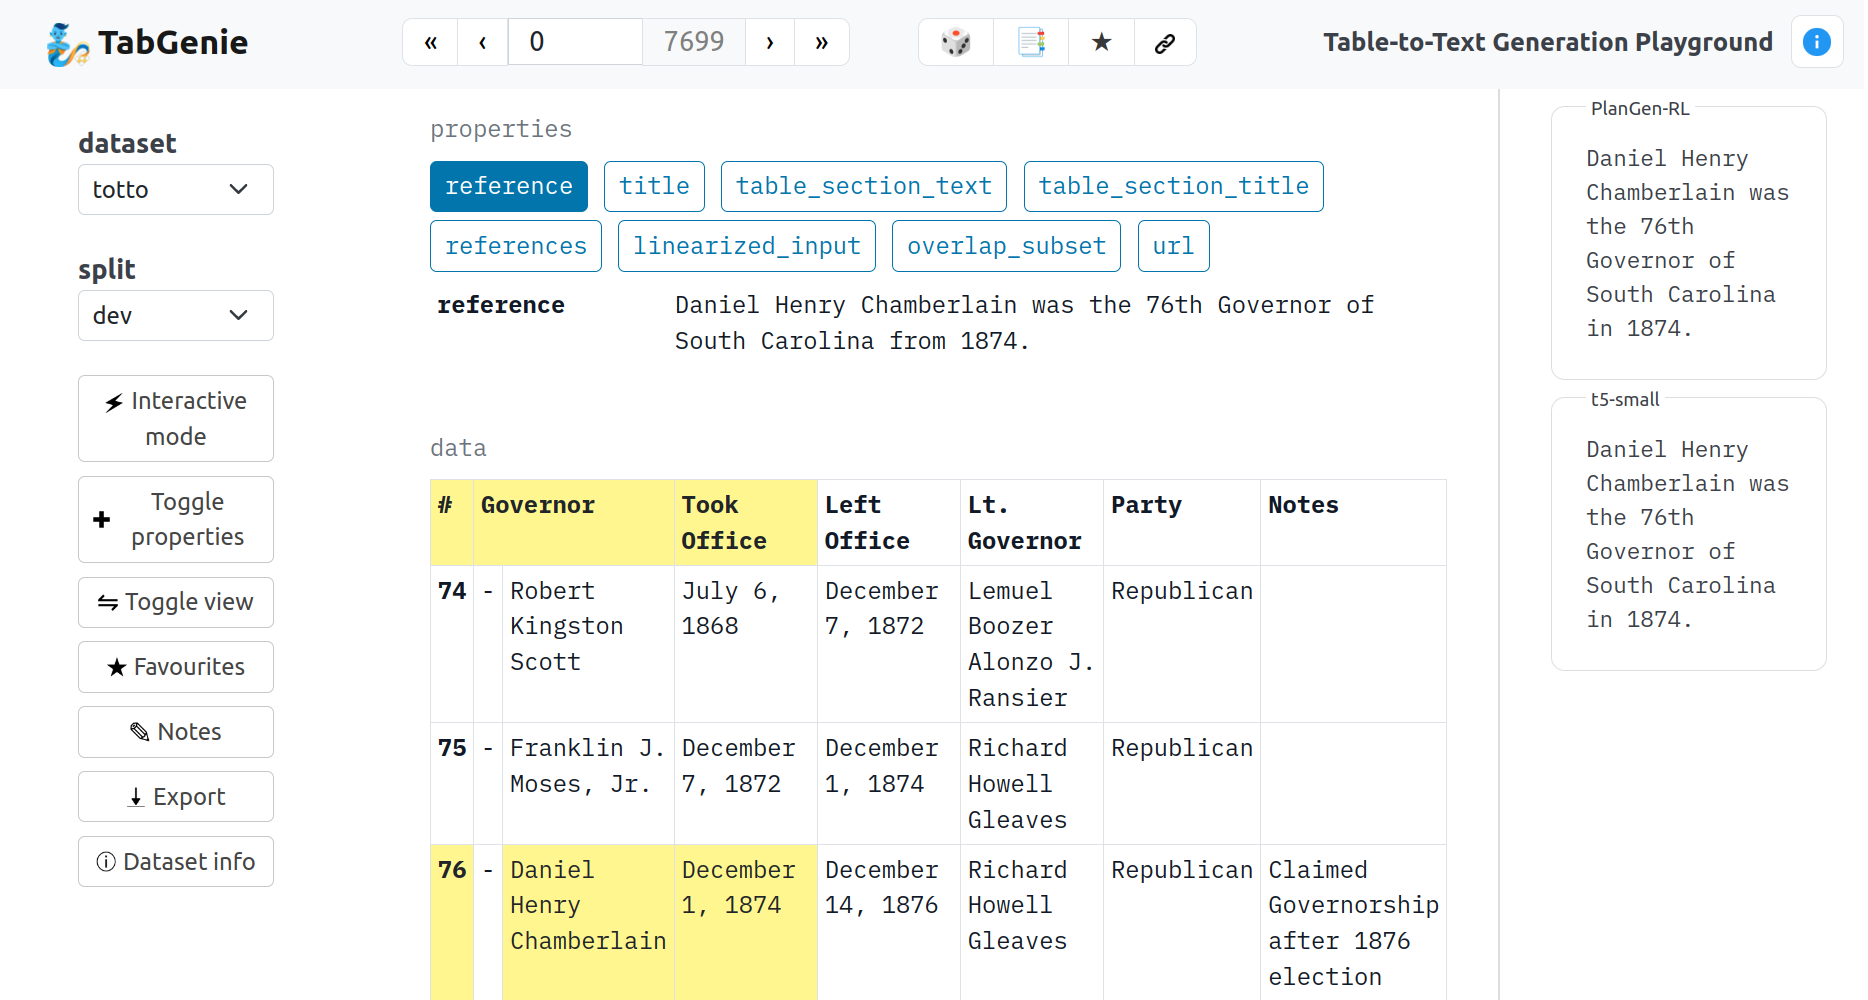
\includegraphics[width=1.0\textwidth]{img/tabgenie_web.png}}
    \caption{The web interface of \textsc{TabGenie}. The \emph{left panel} and the \emph{navigation bar} contains user controls; the \emph{center panel} shows table properties and table content; the \emph{right panel} contains system outputs.}
    \label{fig:tabgenie:web}
\end{figure*}
Input data in \textsc{TabGenie} is in tabular format. We define a \textit{table} as a two-dimensional matrix with $m$ columns and $n$ rows, which together define a grid of $m \times n$ cells. Each cell contains a (possibly empty) text string. A continuous sequence of cells $\{c_{i}, \ldots, c_{i+k}\}$ from the same row or column may be merged, in which case the values of $\{c_{i+1},\ldots,c_{i+k}\}$ are linked to the value of $c_{i}$.  A cell may be optionally marked as a \textit{heading}, which is represented as an additional property of the cell.\footnote{The headings are typically located in the first row or column, but may also span multiple rows or columns and may not be adjacent.}

To better accommodate the format of datasets such as ToTTo \cite{parikhToTToControlledTableToText2020} or HiTab \cite{chengHiTabHierarchicalTable2021}, we also allow individual cells to be \textit{highlighted}. Highlighted cells are assumed to be preselected for generating the output description. The tables may be accompanied with an additional set of properties (see \autoref{fig:tabgenie:web})\footnote{An example of such a property is a \textit{``title''} of the table in WikiBio \cite{lebretNeuralTextGeneration2016} or a \textit{``category''} in WebNLG \cite{gardentWebNLGChallengeGenerating2017}.}, which we represent as key-value pairs alongside the table. The properties may be used for generating the table description.

\paragraph{Unifying Data Format} Our \ac{d2t} generation datasets contain three high-level input data formats: tables, \acs{rdf}\glsunset{rdf} triples, and key-value pairs. We note that converting the latter two to tabular format requires only minimal changes to the data structure while allowing a unified data representation and visualization. We make a few minor changes to datasets which do not immediately adhere to the tabular format:

\begin{itemize}
    \item For graph-to-text datasets, we format each triple as a row, using three columns labeled \textit{subject}, \textit{predicate}, and \textit{object}.
    \item For key-value datasets, we use two-column format, with keys used as row headings in the first column.
    \item For SportSett:Basketball \cite{thomson2020sportsett}, we merge the \textit{box score} and \textit{line score} tables and add appropriate headings where necessary.
\end{itemize}

% Moreover, for ToTTo \citep{parikhToTToControlledTableToText2020}, we also provide our custom, improved header cells highlighting (details are given in Appendix \ref{appendix:totto_highlights}).


\paragraph{Datasets}
We include 16 datasets listed in \autoref{tab:datasets} in \textsc{TabGenie}, covering many subtasks of \ac{d2t} generation. All the datasets are available under a permissive open-source license. To ease the data distribution, we load all the datasets using the Huggingface \texttt{datasets} package \cite{lhoest2021datasets}, which comes equipped with a data downloader. We publicly added to Huggingface \texttt{datasets} 9 out of 16 datasets which were not yet available.\footnote{See \url{https://huggingface.co/datasets?search=kasnerz}.} A custom dataset can be added to \textsc{TabGenie} by simple sub-classing the data loader class and overriding the method for processing individual entries.

\subsection{Web Interface}
\label{sec:tabgenie:web}

\textsc{TabGenie} offers a way to interact with the datasets through the \textit{web interface}. The interface features a single-page layout with three panels containing user controls, input data, and system outputs (see \autoref{fig:tabgenie:web}).

\paragraph{Content Exploration} \textsc{TabGenie} renders input data as HTML tables, providing better visualizations than existing data viewers, especially in the case of large and hierarchical tables.\footnote{Compare, e.g., with the ToTTo dataset in Huggingface Datasets for which the table is provided in a single field called \textit{``table''}: \url{https://huggingface.co/datasets/totto}.} Users can navigate through individual examples in the dataset sequentially, access an example using its index, or go to a random example. The users can add notes to examples and mark examples as favorites for accessing them later. The interface also shows the information about the dataset (such as its description, version, homepage, and license) and provides an option to export the individual examples.

\paragraph{Interactive Mode} In the interactive mode, the user can modify the input data and observe how changes influence model outputs. We assume that the model is running externally and provides access through an \acs{api} which is queried by \textsc{TabGenie}. The user can highlight different cells, edit cell contents, and edit parameters of the downstream processor.

% For example,  The contents of a table are processed by a processing \textit{pipeline}. This pipeline takes table contents and properties as input, processes them with a sequence of modules, and outputs HTML code. The modules are custom Python programs which may be re-used across the pipelines.

% \textsc{TabGenie} currently provides two basic pipelines: (1) calling a generative language model through an API with a custom prompt, and (2) generating graph visualizations of RDF triples. We describe a case-study for the model API pipeline in §\ref{sec:cs:prompting}. Users can easily add custom pipelines by following the instructions in the project repository.

\paragraph{Pre-generated Outputs} \textsc{TabGenie} also allows to visualize static pre-generated outputs, which are loaded in the JSONL\footnote{\url{https://jsonlines.org}} format from a specified directory. Multiple outputs can be displayed alongside a specific example, allowing to compare outputs from multiple systems.


\subsection{Developer Tools}
\label{sec:tabgenie:developer}
Beside the web interface, \textsc{TabGenie} also provides developer-friendly access through Python bindings and a command-line interface. Both of these interfaces aim to simplify dataset preprocessing in downstream tasks. The key benefit of using \textsc{TabGenie} is that it provides streamlined access to data in a consistent format, removing the need for dataset-specific code for extracting information such as table properties, references, or individual cell values.



\paragraph{Python Bindings} \textsc{TabGenie} can replace custom preprocessing code in Python codebases. With a single unified interface for all the datasets, the \textsc{TabGenie} wrapper class allows to:
\begin{itemize}
    \item load a dataset from the Huggingface Datasets or from a local folder,
    \item access individual table cells and their properties,
    \item linearize tables using pre-defined or custom functions,
    \item prepare the Huggingface \texttt{Dataset} objects for downstream processing.
\end{itemize}
\textsc{TabGenie} can be installed as a Python package, making the integration simple and intuitive.

\paragraph{Command-line Tools} \textsc{TabGenie} supports several basic commands via command line:
\begin{itemize}
    \item \textbf{Run} The \texttt{tabgenie run} command launches the local web server, mimicking the behavior of \texttt{flask run}.

          \noindent Example usage:
          % \begin{noindent}
\begin{bash}
tabgenie run --port=8890 --host="0.0.0.0"
\end{bash}
% \end{noindent}
    \item \textbf{Export} The \texttt{tabgenie export} command enables batch exporting of the dataset. The supported formats are \texttt{xlsx}, \texttt{html}, \texttt{json}, \texttt{txt}, and \texttt{csv}. Except for \texttt{csv}, table properties can be exported along with the table content.

          \noindent Example usage:
          % \begin{noindent}
\begin{bash}
tabgenie export --dataset "webnlg" \
    --split "dev" \
    --out_dir "export/datasets/webnlg" \
    --export_format "xlsx"
\end{bash}
% \end{noindent}
          \noindent Export can also be done in the web interface.
    \item \textbf{Spreadsheet} For error analysis, it is common to select $N$ random examples from the dataset along with the system outputs and manually annotate them with error categories. The \texttt{tabgenie sheet} command generates a suitable spreadsheet for this procedure.

          \noindent Example usage:
          % \begin{noindent}
\begin{bash}
tabgenie sheet --dataset "webnlg" \
    --split "dev" \
    --in_file "out-t5-base.jsonl" \
    --out_file "analysis_webnlg.xlsx" \
    --count 50
    \end{bash}
% \end{noindent}
\end{itemize}


\subsection{Implementation}
\label{sec:tabgenie:architecture}

\textsc{TabGenie} runs with Python >=3.8 and requires only a few basic packages as dependencies. It can be installed as a stand-alone \texttt{tabgenie} module from PyPI or from the project repository.

\paragraph{Backend} The web server is based on \texttt{Flask},\footnote{\url{https://pypi.org/project/Flask/}} a popular lightweight Python-based web framework. The server runs locally and can be configured with a YAML\footnote{\url{https://yaml.org}} configuration file. On startup, the server loads the data using the \texttt{datasets}\footnote{\url{https://pypi.org/project/datasets/}} package. To render web pages, the server uses the \texttt{tinyhtml}\footnote{\url{https://pypi.org/project/tinyhtml/}} package and the Jinja\footnote{\url{https://jinja.palletsprojects.com/}} templating language.

\paragraph{Frontend} The web frontend is built on HTML5, CSS, Bootstrap,\footnote{\url{https://getbootstrap.com/}} JavaScript, and jQuery.\footnote{\url{https://jquery.com}} We additionally use the D3.js\footnote{\url{https://d3js.org}} library for visualizing the structure of data in graph-to-text datasets. To keep the project simple, we do not use any other major external libraries.


\subsection{Case Studies}
\label{sec:tabgenie:casestudies}

We present several case-studies for using \textsc{TabGenie} in \ac{d2t} generation research. The instructions and code samples for these tasks are available in the project repository.

\paragraph{Table-To-Text Generation} \textsc{TabGenie} can serve for finetuning a sequence-to-sequence language model for table-to-text generation in PyTorch \cite{paszke} using the Huggingface Transformers \cite{wolf2019HuggingFacesTS} framework. In a typical finetuning procedure, the user needs to prepare a \texttt{Dataset} object with tokenized input and output sequences. Using \textsc{TabGenie}, preprocessing a specific dataset is simplified to the following:
% \begin{noindent}
\begin{python}
from transformers import AutoTokenizer
import tabgenie as tg

# instantiate a tokenizer
tokenizer = AutoTokenizer.from_pretrained(...)

# load the dataset
tg_dataset = tg.load_dataset(
    dataset_name="totto"
)

# preprocess the dataset
hf_dataset = tg_dataset.get_hf_dataset(
    split="train",
    tokenizer=tokenizer
)
\end{python}
% \end{noindent}
The customizable function \texttt{get\_hf\_dataset()} linearizes the tables  and tokenizes the inputs and references. For training a single model on multiple datasets in a multi-task learning setting \cite{xieUnifiedSKGUnifyingMultiTasking2022}, the user may preprocess each dataset individually, prepending a dataset-specific task description to each example. The datasets may then be combined using the methods provided by the \texttt{datasets} package.

\paragraph{Interactive Prompting} \textsc{TabGenie} can be used for observing the impact of various inputs on the outputs of a \ac{llm} prompted for table-to-text generation. The user customizes the provided \texttt{model\_api} pipeline to communicate with a \ac{llm} through an API. The API can communicate either with an external model (using e.g. OpenAI API\footnote{\url{https://openai.com/api/}}), or with a model running locally (using libraries such as FastAPI\footnote{\url{https://fastapi.tiangolo.com}}). The user then interacts with the model through \textsc{TabGenie} web interface, modifying the prompts, highlighted cells, and table content.

\paragraph{Error Analysis} \textsc{TabGenie} can help with annotating error categories in the outputs from a table-to-text generation model. The user generates the system outputs and saves the outputs for a particular dataset split in a JSONL format. Through the command-line interface, the user will then generate a XLSX file which can be imported in any suitable office software and distributed to annotators for performing error analysis.

\chapter{Examining Model Behavior}
\label{chap:investigating}

In this chapter, we observe behaviors of neural \acp{lm} in specific \ac{d2t} generation scenarios, building upon custom datasets.

In \autoref{sec:rel2text}, we examine the capabilities of \acp{plm} to describe unseen relations between entities in knowledge graphs. For this problem, existing \ac{d2t} datasets are not able to discern memorization from generalization. We thus collect a custom dataset with a large variety of relation labels, including unseen labels in the test set. Using our dataset, we investigate whether the models can correctly describe the relations they have not seen in the training data. We find out that the models can generalize unseen labels as long as the labels are human-readable and unambiguous, which is often (but not always) fulfilled in real-world data.

In \autoref{sec:quintd}, we investigate the abilities of open \acp{llm} for \ac{d2t} generation from common formats such as JSON, CSV, and Markdown. To prevent data contamination, we scrape unlabeled data from public sources across five domains. Using \ac{llm}-based referenceless metric and human annotators, we quantify the semantic accuracy of the generated texts with respect to the input data. We find out that although the descriptions are fluent, most of them contain semantic errors.

\section{Describing Relations in Knowledge Graphs}
\label{sec:rel2text}
\begin{refbox}
    This section is based on the paper \emph{Mind the Labels: Describing Relations in Knowledge Graphs With Pretrained Models} \cite{kasnerMindLabelsDescribing2022}, joint work with Ioannis Konstas and Ondřej Dušek. The work was published in the Proceedings of the 17th Conference of the European Chapter of the Association for Computational Linguistics (EACL 2023). The project was led by the author of the thesis; Ioannis Konstas and Ondřej Dušek supervised the project.
\end{refbox}
We investigate how human-readable data labels help \acp{plm} with \ac{d2t} generation. We start by noticing that \acp{plm} can use labels such as column headings, keys, or relation names to generalize to out-of-domain examples. The question is (a) whether this ability is robust enough and (b) how accurate the outputs are in cases where these labels are ambiguous or incomplete. To answer this question, we focus on describing a relation between two entities.

For our experiments, we collect \textsc{Rel2Text}: a novel dataset for verbalizing a diverse set of 1,522 unique relations from three large-scale knowledge graphs (Wikidata, DBPedia, YAGO). We evaluate model outputs on unseen relations using a combination of automatic metrics and manual analysis. We find that although \acp{plm} for D2T generation expectedly fail on unclear cases, models trained with a large variety of relation labels are surprisingly robust in verbalizing novel, unseen relations. We argue that using data with a diverse set of clear and meaningful labels is key to training D2T generation systems capable of generalizing to novel domains. We release the code and data for our experiments on Github.\footnote{\url{https://github.com/kasnerz/rel2text}}


% 
% In this paper, 

\subsection{Motivation}
\ac{d2t} generation systems need to accurately capture the semantics of relations between values in the data. However, the data labels such as relation names \cite{farber2018linked,haller2022analysis}, table headings \cite{parikhToTToControlledTableToText2020}, or meaning representation keys \cite{dusekEvaluatingStateoftheartEndtoEnd2020} may provide only superficial or---if the labels are abbreviations, such as in the Rotowire dataset \cite{wiseman2017challenges}---no usable hints about the data semantics.


% \begin{figure}[t]

\begin{table}[t!] \small
    \centering
    \begin{tabular}{llp{3.7cm}l} \toprule
        \textbf{label}    & \textbf{property id}                                       & \textbf{verbalization}                                               & \textbf{note}                       \\ \midrule
        \textit{part of}  & \href{https://www.wikidata.org/wiki/Property:P361}{P361}   & \eh{} is part of \et{}.                                              & can be used verbatim                \\\cdashlinelr{1-4}
        \textit{duration} & \href{https://www.wikidata.org/wiki/Property:P2047}{P2047} & \eh{} lasted for \et{}.                                              & unambiguous verbalization           \\\cdashlinelr{1-4}
        \textit{platform} & \href{https://www.wikidata.org/wiki/Property:P400}{P400}   & \eh{} is available on \et{}.\newline\eh{} runs on \et{}.             & multiple equivalent lexical choices \\\cdashlinelr{1-4}
        \textit{occupant} & \href{https://www.wikidata.org/wiki/Property:P466}{P466}   & \et{} is occupied by \eh{}.\newline\eh{} plays at \et{}.             & semantics depends on entities       \\\cdashlinelr{1-4}
        % \textit{country}  & \href{https://www.wikidata.org/wiki/Property:P17}{P17}     & \eh{} was born in \et{}. \newline \eh{} is located in \et{}.         & semantics depends on entities       \\\cdashlinelr{1-4}
        \textit{parent}   & \href{https://www.wikidata.org/wiki/Property:P8810}{P8810} & \eh{} is the parent of \et{}. \newline \et{} is the parent of \eh{}. & ambiguous relation direction        \\\bottomrule
    \end{tabular}
    \captionof{table}{Example relation labels and the variability in their verbalizations. \eh{} and \et{} denote subject and object in the triple, respectively. The Wikidata page for each relation is available at \url{https://www.wikidata.org/wiki/Property:<property_id>}.}
    \label{tab:rel2text:example}
\end{table}

\acp{plm} such as BART \cite{lewisBARTDenoisingSequencetoSequence2019} or T5 \cite{raffelExploringLimitsTransfer2019} can quickly adapt to new domains and exhibit robustness to out-of-domain inputs. We investigate to what extent are \acp{plm} limited by the expressivity of the data labels. A suitable testing ground is the task of describing individual \acs{rdf}\glsunset{rdf} triples in a \ac{kg}, as shown in \autoref{tab:rel2text:example}. In this task, there is a wide range of lexical choices for the relation label, while the entities can be copied verbatim or with only minor morphological changes. To illustrate the problem, consider the last example in \autoref{tab:rel2text:example}: the model can use its representation of \emph{``parent''} to understand there is a \emph{``is-a-parent-of''} relation between the entities, but it has to infer (or guess) who is the parent of whom. Even in less ambiguous cases, the model still has to correctly capture the intended semantics of the relation (e.g. \emph{``occupant''} meaning \emph{``home team''}).


Current human-annotated datasets for \ac{d2t} generation are not suitable for investigating this problem, as they contain only a small number of relations and rarely contain any unseen relations in the test set \cite{mille2021automatic}. The only existing datasets covering verbalizations of a wider range of \ac{kg} relations are based on \emph{model-generated outputs} \cite{agarwalKnowledgeGraphBased2021,amaral2022wdv}. For this reason, we collect a novel human-annotated dataset for the task.

Our aim is also to investigate whether incorporating long-form \emph{descriptions} of data labels helps improve model outputs. Previous works have reached contradictory conclusions: \citet{wang2021kepler} use descriptions of relations instead of their labels for relation embeddings, concluding that it results in worse performance on downstream tasks. Conversely, \citet{kale-rastogi-2020-template} and \citet{lee2021dialogue} improve the performance of their systems by including schema descriptions on the input for the dialogue state tracking and dialogue response generation systems.

Lastly, we investigate \emph{verbalizing single triples} as a stand-alone task. As we have shown (\Cref{sec:iterative,sec:pipeline,sec:sem-acc}), in line with other works \cite{xiangASDOTAnyShotDatatoText2022,kale-rastogi-2020-template,gupta2020infotabs,neeraja2021incorporating}, transforming triples to text helps for \acp{plm}-based data processing. The works above use various methods for converting individual triples to text, ranging from simple templates and rule-based systems to prompting \acp{plm}; however, none of them investigate how to apply these approaches to novel relations.


% 

% Using the \textsc{Rel2Text} dataset, we evalute the ability of \acp{plm} to verbalize relations which were not present in the training set. We consider both models finetuned on other relations in our dataset and models finetuned on datasets from a related domain. We also experiment with scenarios involving few-shot finetuning, training on masked labels, and extending the labels with descriptions (§\ref{sec:analysis},~\ref{sec:results}).

% We find that the \acp{plm} are quite robust in verbalizing a diverse set of relations based on their label (achieving \textasciitilde 90\% of overall entailment probability). We show that semantically unfaithful model outputs are often caused by incomplete, ambiguous, or noisy input data.



% Somewhat suprisingly, we also show that longer relation descriptions do not provide substantial improvements over using short labels.  

% However, even for data using short relation labels, the model trained on verbalizing relations can achieve results comparable to verbalizing relations using manual templates in two downstream tasks (§\ref{sec:downstream}).



\subsection{\textsc{Rel2Text} dataset}
\label{sec:rel2text:data}
For our experiments, we need data with diverse labels and their human verbalizations. We start by collecting a large set of relations from three large-scale \acp{kg} (Wikidata, DBPedia, and YAGO). For each relation, we collect its label, textual description, and up to five triples in which the relation occurs in the \ac{kg}. We then use human annotators to collect a \emph{verbalization} for each triple, i.e., a short sentence capturing the meaning of the triple. After filtering, our dataset---which we call \textsc{Rel2Text} (\underline{R}e-writing \underline{e}dge \underline{l}abels to Text)\footnote{Or simply ``Relations-to-Text''.}---contains 4,097 single triples covering 1,522 unique relations. We describe the data collection process in the following paragraphs.


\paragraph{Input Data}
An \acs{rdf} triple is a tuple $t = (s, r, o)$, where $r$ denotes the relation\footnote{In previous sections, we have also called this constituent a \emph{predicate}; these notions are equivalent.} between the subject $s$ and the object $o$.
We retrieve triples from three open large-scale \acp{kg} encoding factual knowledge:

\begin{itemize}
    \item \textbf{Wikidata} \cite{vrandevcic2014wikidata} is a large-scale Wikipedia-based \ac{kg} created using collaborative editing. With approximately 10,000 human-created relations equipped with descriptions\footnote{\url{https://www.wikidata.org/wiki/Wikidata:Database_reports/List_of_properties/all}}, it is by far the largest source of variety in relation labels.
    \item \textbf{YAGO} \cite{pellissier2020yago} is a \ac{kg} which builds upon factual knowledge from Wikidata, but uses a limited set of 116 pre-defined relations from \texttt{schema.org} \cite{guha2016schema} mapped to a subset of Wikidata relations.
    \item \textbf{DBPedia} \cite{auer2007dbpedia,lehmann2015dbpedia} is a \ac{kg} that maps Wikipedia infotables to a predefined ontology containing 1,355 relations, about 350 of which are accompanied by a description.
\end{itemize}

We query all \acp{kg} using their openly available endpoints to retrieve a list of relations in each \ac{kg}. For each relation, we retrieve up to five \textit{triples} that use this relation and the relation \textit{description}, i.e., a short explanatory text.
If present, we also retrieve descriptions for the subject and the object.

We apply a set of filtering heuristics, leaving out, e.g., relations describing \ac{kg} metadata or identification numbers.\footnote{Relations describing various IDs make up a large portion of relations in Wikidata. Since we focus on diversity instead of coverage, we decided not to include these relations in our dataset.} In this way, we collect 7,334 triples with 1,716 relations in total.

\paragraph{Annotation Process}
We collect human-written verbalizations for all input triples using Prolific.\footnote{\url{https://www.prolific.co/}} We built a web interface where human annotators are shown a single triple $t$ and asked to describe it in a single sentence. The annotators are encouraged to re-use the entities in their original form, but they can change the form if necessary. The annotators can also report noisy inputs. We employed 420 annotators in total, each of which annotated 20 examples. We set the average reward per hour according to the platform recommendations to  \textsterling{}7.29 per hour, and we accepted all the inputs that passed our built-in checks.

\paragraph{Postprocessing the Data}
A considerable portion of the collected verbalizations contain typos and grammatical errors, misunderstood meaning of the relation, or extra information in the input. To ensure the high quality of our data, we manually examined all crowdsourced examples and annotated them as \textit{OK}, \textit{noisy}, \textit{corrupted}, or \textit{containing extra information}. For our experiments, we only use the subset of our dataset with \textit{OK} annotations, one per input triple (4,097 examples, 1,522 distinct relations).


\subsection{Analysis and Experiments}
\label{sec:rel2text:analysis}
In our analysis, we are interested in the following research questions:
\begin{itemize}
    \item \textbf{RQ1:} Are the PLMs finetuned for D2T generation able to describe relations \textit{not present in the finetuning corpus}?
    \item \textbf{RQ2:} How many \textit{training examples} do the PLMs need to generate satisfactory outputs?
    \item \textbf{RQ3:} How do the PLMs behave when provided \textit{limited lexical cues} about the relation?
    \item \textbf{RQ4:} Can relation \textit{descriptions} help to clarify ambiguous cases and improve the semantic accuracy of the outputs?
\end{itemize}

\paragraph*{Datasets}  We experiment with the following datasets, all of which focus on verbalizing factual information from \acp{kg} and use the same triple-based input data format:
\begin{itemize}
    \item \textsc{Rel2Text}: Our dataset with single triples from three \acp{kg} with 4,097 examples, 1,522 relations, and \textit{human-annotated} outputs.
    \item WebNLG \cite{ferreira20202020,gardentWebNLGChallengeGenerating2017}: A DBPedia-based triple-to-text dataset with 38k examples, 411 relations, up to 7 triples per example, and \textit{human-annotated} outputs. We use the English part of version 3.0 from HuggingFace.\footnote{\url{https://huggingface.co/datasets/web_nlg}}
    \item KeLM \cite{agarwalKnowledgeGraphBased2021}: A Wikidata-based dataset with 11M examples, 1,519 relations, up to 13 triples per example, and \textit{model-generated} outputs. We use the dataset released by the authors, splitting it into a 1:100 ratio for validation and training data.
\end{itemize}
To answer the research questions, we divide our \textsc{Rel2text} dataset into a training and test split. We then use the \textsc{Rel2Text} \emph{test set} to evaluate a finetuned BART model \cite{lewisBARTDenoisingSequencetoSequence2019}. To answer \emph{RQ1}, we compare the performance of BART finetuned on the \textsc{Rel2Text} training set with BART finetuned on WebNLG and KeLM. Using \textsc{Rel2text} only, we then prepare various setups for answering \emph{RQ2}, \emph{RQ3}, and \emph{RQ4}.


\paragraph{Rel2Text Data Split} We use approximately 15\% of the \textsc{Rel2Text} examples for the \emph{test set}. To ensure maximum fairness and focus on model generalization to unseen relations, we do not include in the \textsc{Rel2Text} test set any relations that have an exact string match with a relation in KeLM, WebNLG, or the \textsc{Rel2Text} training set. We also exclude any relations for which the maximum semantic similarity\footnote{Computed as cosine similarity between embeddings of the labels, which are encoded using \texttt{all-distilroberta-v1} from SBERT \cite{reimers-gurevych-2019-sentence}.} to any KeLM/WebNLG/\textsc{Rel2Text} training relation exceeds a threshold of $0.9$. We set this threshold empirically to exclude relations that are almost synonymous, but slightly lexically different.
We use 90\% of the remaining examples for the training set and 10\% for the validation set.

\paragraph{Experimental Setup} We split the camel case in the relation labels. For finetuning the models, we linearize the input triples by marking the triple constituents with special tokens that we add to the model vocabulary. In a default scenario, we finetune BART-base \cite{lewisBARTDenoisingSequencetoSequence2019} for 10 epochs and select the best checkpoint using validation BLEU score, then use greedy decoding to produce outputs. We repeat each experiment with five random seeds, averaging the results.


\paragraph{Compared Systems} We compare the following systems:
\begin{itemize}
    \item \textbf{Copy Baseline}: We introduce a simple \textit{copy} baseline by outputting the triple constituents separated by space: ``$s\text{ }r\text{ }o$''.



    \item \textbf{Full Training Data}: We use the default setup on full \textsc{Rel2Text} and WebNLG training sets. For KeLM (which is about 300$\times$ larger than WebNLG), we finetune the model only for one epoch. We denote the trained models \BARTr{}, \BARTw{}, and \BARTk{}, respectively.

    \item \textbf{Limited Training Data}: For the limited training data setup, we prepare few-shot splits from \textsc{Rel2Text} as subsets containing $N=$ \{25, 50, 100, 200\} relations with a single example per relation. We select examples at random, ensuring that each few-shot split is a subset of the larger splits. We finetune the \textit{fewshot-N} models for 10 epochs without validation, using the last checkpoint.

    \item \textbf{Limited Lexical Cues}: We investigate how the models behave if we do not include the relation labels at all. We consider three scenarios:
          \begin{itemize}
              \item \textit{mask-test} -- We train the model on \textsc{Rel2Text} in the standard training setup. For testing, we replace the relation labels in  \textsc{Rel2Text} with the \textit{<mask>} token.
              \item \textit{mask-train} -- For training, we replace the relation labels in  \textsc{Rel2Text} with the \textit{<mask>} token. We test the model on \textsc{Rel2Text} in the standard evaluation setup.
              \item \textit{mask-all} -- We replace the relation labels in  \textsc{Rel2Text} with the \textit{<mask>} token for both training and testing.
          \end{itemize}


    \item \textbf{Incorporating Descriptions}: Our dataset contains short textual descriptions of the relations, which may be useful to disambiguate its meaning and provide additional cues to the model. We consider two scenarios:
          \begin{itemize}
              \item \textit{desc-repl} -- We replace the relation label with its description.
              \item \textit{desc-cat} -- We concatenate the relation description with the input, separated using the special token \textit{<rel\_desc>}.
          \end{itemize}
\end{itemize}

\subsection{Evaluation Setup}
\paragraph{Automatic Metrics}


We evaluate generated outputs using an extensive set of automatic metrics from the GEM-metrics\footnote{\url{https://github.com/GEM-benchmark/GEM-metrics}} package \cite{gehrmannGEMBenchmarkNatural2021}. We use BLEU \cite{papineni2002bleu}, \mbox{METEOR} \cite{banerjee-lavie-2005-meteor}, and BLEURT \cite{sellam2020bleurt} for measuring lexical similarity. For semantic similarity, we use NUBIA \cite{kaneNUBIANeUralBased2020} along with its individual features: the semantic similarity score (SS) on a 0-5 scale, the contradiction (C), neutral (N), and entailment (E) probabilities, and the perplexity score (PPL). To assess lexical diversity, we measure the number of unique n-grams (U-1), conditional entropy of bi-grams (CE2), and the mean segmental type-token ratio over segment lengths of 100 (MSTTR). We also measure the average output length in tokens (len). See \autoref{sec:evaluation} for a detailed description of the metrics.



\paragraph{Manual Error Analysis} Based on our preliminary observations, we identify four sources of model errors: semantic errors (\textsc{Sem}), with a swap of the relation direction (\textsc{Dir}) as a special case, too literal (\textsc{Lit}), i.e., containing awkward or misleading phrasing, and grammar/lexical errors (\textsc{Lex}). We further identified two types of input data errors: ambiguous relations (\textsc{Ent}) and relations with unclear labels (\textsc{Lbl}). Examples are shown in \autoref{tab:rel2text:cat}.
For error analysis, we select 100 random examples together with their corresponding outputs from the \textit{\BARTr}, \textit{\BARTw}, \textit{\BARTk}, \textit{fewshot-100}, \textit{mask-all} and \textit{desc-cat} models. Without revealing the output sources, we mark all error categories that apply.
\begin{table*}[t]
    \centering\footnotesize
    % \setlength{\tabcolsep}{4pt}
    % \renewcommand{\arraystretch}{1.25}
    \begin{tabular}{p{0.5cm}p{1cm}p{11.6cm}} \toprule

         & \textbf{Label} & \textbf{Example inputs and outputs (\red{\xmark} incorrect, \green{\cmark} correct)}                                                                                                                                                                                    \\ \midrule
        %
        \multirow{12}{*}{\rotatebox[origin=c]{90}{\textit{model}}}
        % 
         & \textsc{Sem}   & \emph{(Yousra Matine, sport country, Morocco)} \newline \red{\xmark} Yousra Matine was born in Morocco. [\emph{mask-mask}] \newline  \green{\cmark} Yousra Matine plays for Morocco. [\BARTr]                                                                           \\[2mm]
         & \textsc{Dir}   & \emph{(Kentucky Channel, former broadcast network, KET ED)} \newline \red{\xmark} KET ED was broadcast on Kentucky Channel ED. [\emph{fewshot-100}] \newline  \green{\cmark} The Kentucky Channel was broadcast on KET ED. [\BARTr]                                     \\[2mm]
         & \textsc{Lit}   & \emph{(Vietnam Television, first air date, 1970-09-07)} \newline \red{\xmark} The first air date of Vietnam Television was 1970-09-07. [\BARTk] \newline  \green{\cmark} Vietnam Television first aired on 1970-09-07. [\BARTr]                                         \\[2mm]
         & \textsc{Lex}   & \emph{(RPG-43, used in war , The Troubles)} \newline \red{\xmark} RPG-43 was used in the The Troubles. [\BARTr] \newline  \green{\cmark} The RPG-43 was used in the Troubles. [\BARTk]                                                                                  \\[1mm]\cdashlinelr{1-3}\\[-3mm]
        %
        \multirow{6}{*}{\rotatebox[origin=c]{90}{\textit{data}}}
        %
         & \textsc{Ent}   & \emph{(The Age of Entitlement, by artist, The Basics)} \newline \red{\xmark} The Age of Entitlement was written by The Basics. [\BARTk] \newline  \green{\cmark} The Age of Entitlement was recorded by The Basics.  [\BARTr]                                           \\[2mm]
         & \textsc{Lbl}   & \emph{(General Motors Epsilon platform, vehicle, Cadillac XTS)} \newline \red{\xmark} General Motors Epsilon is a vehicle similar to the Cadillac XTS. [\BARTw] \newline  \green{\cmark} General Motors Epsilon platform is used in the Cadillac XTS. [\emph{desc-cat}] \\
        \bottomrule
    \end{tabular}
    \caption{Error categories used in manual analysis, with examples of errors found and corresponding correct verbalizations (square brackets denote the model).
        Model error types (top):
        \textsc{Sem} -- The output is semantically incorrect,
        \textsc{Dir} -- The direction of the relation is swapped,
        \textsc{Lit} -- The verbalization is too literal,
        \textsc{Lex} -- There is a lexical error in the output.
        %
        Input data error types (bottom):
        \textsc{Ent} -- The verbalization may depend on the entities,
        \textsc{Lbl} -- The relation label is not clear.
    }
    \label{tab:rel2text:cat}
\end{table*}


\subsection{Findings from Automatic Metrics}
\label{sec:rel2text:results}

\begin{table*}[t]\centering
    \footnotesize
    \setlength{\tabcolsep}{5pt}
    \begin{tabular}{lc>{\hspace{-2mm}}c>{\hspace{-2mm}}cc>{\hspace{-2mm}}c>{\hspace{-2mm}}c>{\hspace{-2mm}}c>{\hspace{-2mm}}cc>{\hspace{-2mm}}c>{\hspace{-2mm}}c>{\hspace{-2mm}}c>{\hspace{-2mm}}c>{\hspace{-2mm}}c}\toprule
        \multirow{2}{*}{} & \multicolumn{3}{c}{\textbf{Lexical}} & \multicolumn{5}{c}{\textbf{Semantics}} & \multicolumn{5}{c}{\textbf{Referenceless}}                                                                                              \\\cmidrule(r){2-4}\cmidrule(r){5-9}\cmidrule{10-14}
                          & \bf BLEU                             & \bf MET                                & \bf BLR                                    & \bf SS & \bf C & \bf N & \bf E & \bf NB & \bf U-1 & \bf CE-2 & \bf TTR & \bf PPL & \bf len \\\midrule
        \it human         & -                                    & -                                      & -                                          & -      & -     & -     & -     & -      & 1785    & 2.13     & 0.62    & 5.88    & 9.55    \\
        \it copy          & 29.04                                & 37.52                                  & 0.09                                       & 4.79   & 1.22  & 7.57  & 91.21 & 0.74   & 1606    & 1.17     & 0.7     & 7.55    & 6.72    \\\cdashlinelr{1-14}
        \it \BARTr{}      & 52.54                                & 44.86                                  & 0.54                                       & 4.72   & 3.50  & 4.65  & 91.85 & 0.88   & 1661    & 1.96     & 0.58    & 5.89    & 9.16    \\
        \it \BARTw{}      & 41.99                                & 41.59                                  & 0.41                                       & 4.65   & 3.68  & 6.93  & 89.39 & 0.86   & 1651    & 2.54     & 0.56    & 5.65    & 10.29   \\
        \it \BARTk{}      & 46.74                                & 42.94                                  & 0.46                                       & 4.70   & 3.95  & 5.29  & 90.77 & 0.86   & 1652    & 2.32     & 0.56    & 5.83    & 9.71    \\\cdashlinelr{1-14}
        \it fewshot-25    & 31.13                                & 35.52                                  & -0.02                                      & 3.94   & 8.35  & 27.26 & 64.39 & 0.65   & 1445    & 2.93     & 0.52    & 5.34    & 10.67   \\
        \it fewshot-50    & 40.60                                & 40.05                                  & 0.25                                       & 4.44   & 8.04  & 13.12 & 78.84 & 0.76   & 1536    & 2.31     & 0.55    & 5.79    & 9.90    \\
        \it fewshot-100   & 45.88                                & 42.38                                  & 0.38                                       & 4.53   & 6.34  & 10.60 & 83.06 & 0.81   & 1600    & 2.13     & 0.57    & 5.85    & 9.57    \\
        \it fewshot-200   & 48.67                                & 43.34                                  & 0.44                                       & 4.58   & 5.40  & 9.03  & 85.57 & 0.83   & 1626    & 2.04     & 0.58    & 5.89    & 9.36    \\\cdashlinelr{1-14}
        \it mask-test     & 42.45                                & 38.52                                  & 0.25                                       & 3.99   & 14.91 & 18.47 & 66.62 & 0.65   & 1669    & 1.96     & 0.61    & 5.69    & 8.96    \\
        \it mask-train    & 46.90                                & 43.15                                  & 0.43                                       & 4.55   & 5.85  & 11.55 & 82.61 & 0.81   & 1646    & 2.00     & 0.57    & 5.91    & 9.74    \\
        \it mask-all      & 42.53                                & 38.49                                  & 0.24                                       & 3.85   & 17.58 & 25.15 & 57.26 & 0.61   & 1677    & 1.96     & 0.61    & 5.66    & 9.16    \\\cdashlinelr{1-14}
        \it desc-repl     & 49.35                                & 42.85                                  & 0.47                                       & 4.57   & 5.78  & 8.80  & 85.42 & 0.82   & 1693    & 1.94     & 0.59    & 5.86    & 9.18    \\
        \it desc-cat      & 53.07                                & 45.04                                  & 0.55                                       & 4.72   & 3.46  & 4.66  & 91.88 & 0.87   & 1668    & 1.91     & 0.59    & 5.92    & 9.11    \\
        \bottomrule
    \end{tabular}
    \caption{The summary of evaluation using automatic metrics on \textsc{Rel2text} test set. \textbf{MET} = METEOR, \textbf{BLR} = BLEURT, \textbf{TTR} = MSTTR. See \autoref{sec:rel2text:analysis} for the descriptions of the models and metrics.}
    \label{tab:rel2text:auto}
\end{table*}
\autoref{tab:rel2text:auto} shows automatic scores for all our models.

\paragraph{Lexical and Semantic Similarity}
\BARTr{} is the best among the fully trained models regarding lexical overlap metrics, which is expected, as it is trained on the most similar reference distribution. \BARTw{} and \BARTk{} models are almost equal in terms of semantic consistency, achieving around 90\% average entailment probability, which is on par with the copy baseline.

\paragraph{Few-shot Models} For the few-shot models, semantic similarity is much lower (e.g., the average entailment probability is between 65\% and 85\%), showing that there is a certain minimum amount of data needed to achieve consistent outputs. As we show in \autoref{fig:rel2text:fewshot}, using more examples to train the model generally helps decrease variance and increase performance across various metrics.

\paragraph{Masked Relations} Interestingly, the models which do not see the relations during test time (\textit{mask-test} and \textit{mask-all}) still achieve around 60\% average entailment probability, similarly to the worst few-shot model. Although their rate of contradictions is higher than for other models, the results suggest that in many cases, the guessed relation is semantically consisten with the correct relation. Another interesting observation is that the \textit{mask-train} model (trained not to use the labels) can use the labels provided at test time to improve the outputs considerably (contradiction rate drops from 17\% to 5\% compared to \textit{mask-all}).

\paragraph{Influence of Descriptions} The fact that the short labels are both sufficient and necessary for successful verbalization is emphasized by the fact that the \textit{desc-repl} model is worse than \BARTr{} (although the descriptions are longer and supposedly explain the relation semantics). Moreover, the benefits of concatenating the descriptions alongside the relation labels (\textit{desc-cat}) are negligible, only slightly improving lexical similarity metrics (0.5 BLEU point gain over \BARTr{}).

\paragraph{Lexical Diversity} In terms of lexical diversity, human references use more unique n-grams, but the model outputs are very similar in other aspects. It remains to be seen if the model outputs can stay semantically consistent with diversity-focused decoding techniques such as nucleus sampling \cite{holtzman2019curious}.

\begin{figure}[t]
    \centering
    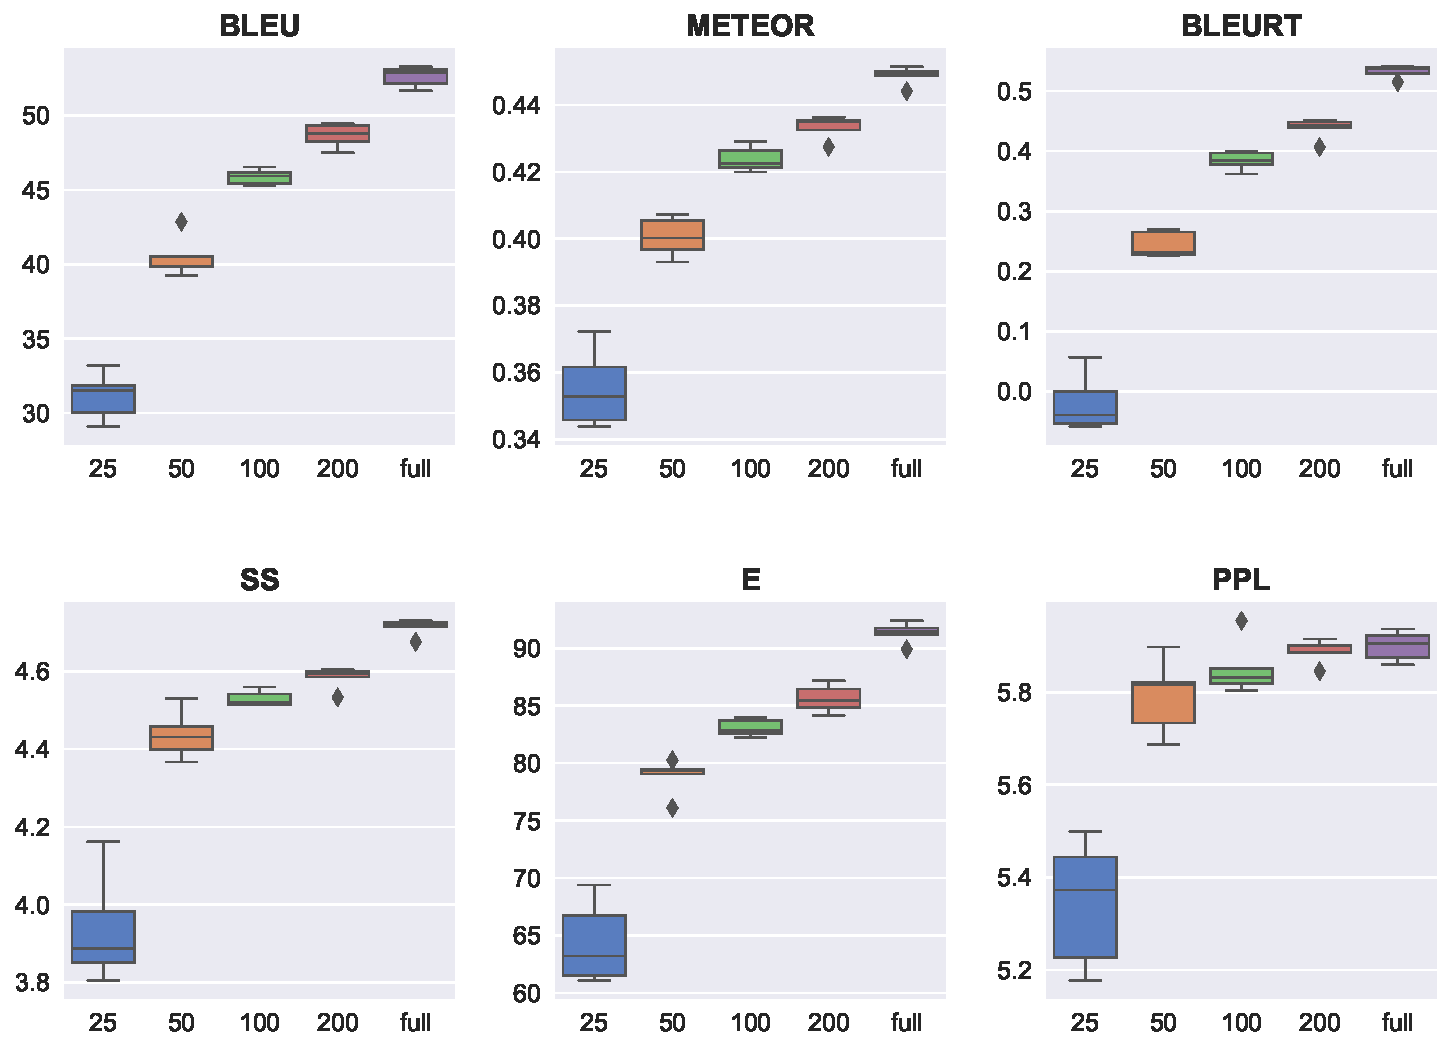
\includegraphics[width=\textwidth]{img/rel2text-fewshot.pdf}
    \caption{Boxplots for selected metrics from \autoref{tab:rel2text:auto} w.r.t. the number of examples (displayed on the \textit{x}-axis, $\textit{full} = 1522$), taking into account variance from individual random seeds.}\label{fig:rel2text:fewshot}
\end{figure}

\subsection{Findings from Manual Error Analysis}


\begin{figure}[t]
    \centering
    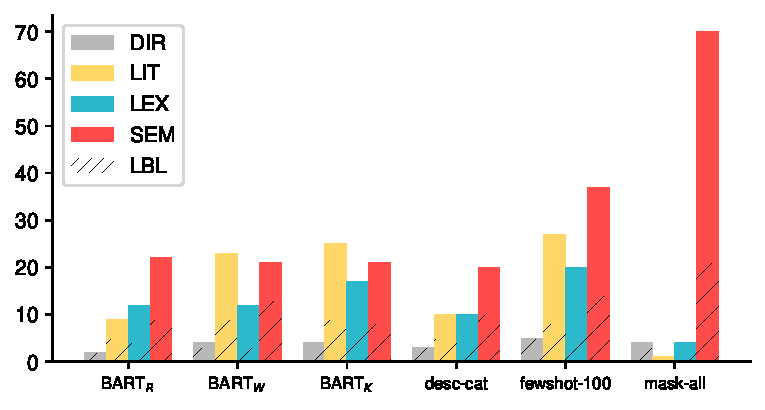
\includegraphics[width=0.7\textwidth]{img/rel2text-graph.pdf}
    \caption{Number of annotated errors per model (see \autoref{tab:rel2text:cat} for the description of error categories and \autoref{sec:rel2text:analysis} for the models). The striped part signifies that the label of the input was marked as unclear.}
    \label{fig:rel2text:manual}
\end{figure}
Results are summarized in \autoref{fig:rel2text:manual}; examples of model outputs for each error type are shown in \autoref{tab:rel2text:cat}.

\paragraph{Naturalness of Expressions} The \BARTk{} and \BARTw{} models use expressions that are too literal (\textsc{Lit}) in 23 and 29 cases, respectively, while the \BARTr{} and \textit{desc-cat} models do the same only in 11 cases (5 out of which are marked as \textsc{Lbl}, i.e., with an unclear label). This suggests that the variability of our dataset helps models to apply more natural expressions, especially if the relation is understandable from its label.

\paragraph{Semantic Errors} There is a near-constant portion of examples where the models make a semantic error (\textsc{Sem}) \textit{and} the input is marked as needing an extra description (\textsc{Lbl}). The models also make relatively many semantic errors, most prominently in the case of the \textit{fewshot-100} and the \textit{mask-all} models. The \textit{mask-all} model made a semantic error in 78 cases, suggesting that guessing the exact relation just from the entities is difficult (although still possible in 22 cases). Moreover, the outcomes from this model are fluent (only 4 \textsc{Lex} errors), making it hard to detect faulty cases.
The case of swapping the relation direction (\textsc{Dir}) is surprisingly not that common, which is probably down to having only a few examples in our dataset prone to this kind of error.

\paragraph{Additional Clues} There were only 12 out of 100 examples annotated as \textsc{Ent}, which suggests that the verbalization of the relation can be mostly decided irrespective of the entities in the triple. Notably, the results for \BARTr{} and \textit{desc-cat} are very similar, rendering the impact of extra descriptions negligible.


\subsection{Applications to Downstream Tasks}
\label{sec:rel2text:downstream}
Given that the \BARTr{} model can describe relations from their labels with high accuracy, we investigate if we can use the model to replace manually created templates in downstream tasks. We select two qualitatively different tasks, both using the idea of transforming individual input triples to simple sentences as a preprocessing step: tabular reasoning and zero-shot data-to-text generation.


\begin{table}[t]\centering
    \small
    \setlength{\tabcolsep}{4pt}
    \begin{tabular}{lcccc}\toprule
        \textbf{premise repr.}              & \textbf{dev} & $\alpha_1$ & $\alpha_2$ & $\alpha_3$ \\\midrule
        OPR \cite{gupta2020infotabs}        & 76.78        & 75.30      & 68.46      & 64.63      \\
        BPR \cite{neeraja2021incorporating} & 77.04        & 74.44      & 67.46      & 63.17      \\
        \BARTr{} (ours)                     & 74.44        & 74.31      & 64.59      & 63.46      \\
        \bottomrule
    \end{tabular}
    \caption{Accuracy for the dev set and test sets  $\alpha_{1,2,3}$ from the \textsc{InfoTabS} dataset. The results are averaged over 3 random seeds.}
    \label{tab:rel2text:nli}
\end{table}


\paragraph{Tabular Reasoning} For the task of \ac{nli} from a table, \citet{gupta2020infotabs} represent each table cell using a simple template \text{``The \textit{key} of \textit{title} are \textit{value}.''}. \citet{neeraja2021incorporating} extend their approach by preparing a fine-grained set of rules\footnote{Formalized using more than 250 lines of Python code: \url{https://github.com/utahnlp/knowledge\_infotabs/blob/main/scripts/preprocess/bpr.py\#L120}} for individual entity categories. We replicate the setup of \citet{neeraja2021incorporating} for the original (OPR) and better (BPR) paragraph representation using their public codebase. We then replace their templates with our \BARTr{} model, verbalizing the triple (\textit{title}, \textit{key}, \textit{value}). The results are summarized in Table \ref{tab:rel2text:nli}. Our manual evaluation suggests that the sentences from our model are indeed more grammatical (even compared to BPR), but we observe comparable performance across all three test sets. In line with \citet{mccoy2019right}, we conclude that for classification tasks such as NLI, the input content appears to be more important than the input form.


\begin{table}[t]\centering
    \small
    \setlength{\tabcolsep}{4pt}
    \begin{tabular}{clcccc}\toprule
        \textbf{dataset}                   & \textbf{model} & \textbf{BLEU} & \textbf{METEOR} & \textbf{O} & \textbf{H} \\\midrule
        \multirow{2}{*}{\textit{filtered}} & orig           & 43.19         & 39.13           & 0.152      & 0.073      \\
                                           & \BARTr{}       & 45.39         & 38.97           & 0.056      & 0.161      \\\cdashlinelr{1-6}
        \multirow{2}{*}{\textit{full}}     & orig           & 42.92         & 39.07           & 0.051      & 0.148      \\
                                           & \BARTr{}       & 44.63         & 38.93           & 0.058      & 0.166      \\
        \bottomrule
    \end{tabular}
    \caption{Lexical similarity metrics (BLEU, METEOR) and ommission (O) and hallucinaton (H) rate; following the setup in \citet{kasner2022neural}.}\label{tab:rel2text:zeroshot}
\end{table}

\paragraph{Zero-shot Data-to-Text Generation} In \autoref{sec:pipeline}, we described our approach for zero-shot D2T generation which requires transforming individual triples into text \cite{kasner2022neural}. Here, we replicate the setup on the WebNLG dataset, applying the \BARTr{} model instead of the templates. The results are summarized in Table \ref{tab:rel2text:zeroshot}.  We note that the pipeline using our model for preprocessing is able to achieve improvements of $\sim$2 BLEU points, at the cost of a slightly higher omission and hallucination rate, but crucially without needing the manual effort to create templates. A cursory examination shows that sentences produced by our model are qualitatively similar to the manual templates but more varied. Unlike the templates, our model may verbalize a relation differently depending on the context.
Overall, we argue that training a PLM on verbalizing individual relations can potentially replace the manual effort of creating simple templates, which will have a notable impact on scaling similar approaches to larger datasets.



\ZK{TODO: discuss ASPIRO: Any-shot Structured Parsing-error-Induced ReprOmpting for Consistent Data-to-Text Generation}


\section{Data-to-Text Generation with Large Language Models}
\label{sec:quintd}

\begin{refbox}
    This section is based on the paper \emph{Beyond Basic Benchmarks: Evaluating Open LLMs on Data-to-Text Generation} \cite{kasnerReferenceBasedMetricsAnalyzing2024}, joint work with Ondřej Dušek. The work \ZK{TODO}
\end{refbox}

% We analyze the behaviors of open \acp{llm} on the task of \ac{d2t} generation. To avoid the issue of \ac{llm} training data contamination with standard benchmarks, we design \datatool{} -- a tool for collecting novel structured data records from public APIs. Using a dataset collected with \datatool and leveraging reference-free evaluation, we analyze model behaviors on five D2T generation tasks.
% We find that recent open \acp{llm} (Llama2, Mistral, and Zephyr) can generate fluent and coherent text from standard data formats in zero-shot settings. However, we also show that the semantic accuracy of the outputs is a major issue: both according to our GPT-4-based metric and human annotators, more than 80\% of the outputs of open \acp{llm} contain a semantic error. We publicly release the code, data, and model outputs at \url{https://d2t-llm.github.io/}.


% Large language models (\acp{llm}; \citealp{ouyang2022TrainingLM,touvron2023llama,touvronLlamaOpenFoundation2023,jiangMistral7B2023,tunstallZephyrDirectDistillation2023}) have already left a mark in many areas of natural language processing (NLP). Surprisingly, their applicability to the task of data-to-text (D2T) generation \cite{reiter1997building,gatt2018survey} remains underexplored, with limited evaluation on a handful of well-established benchmarks only \cite{axelssonUsingLargeLanguage2023,yuanEvaluatingGenerativeModels2023}. Generating text from structured data is arguably challenging for \acp{llm}, given the specifics of D2T generation, such as long inputs, complex non-linear structure, and strict requirements on semantic accuracy. However, a more significant issue is perhaps the lack of testing grounds. The current D2T generation benchmarks are not only getting saturated \cite{vanmiltenburgBarriersEnablingFactors2023}, but also promote optimization towards traditional reference-based evaluation metrics, which were shown to correlate poorly with human judgment \cite{gehrmann2022repairing,vanderleeHumanEvaluationAutomatically2021,novikovaWhyWeNeed2017}. When it comes to the models, using closed \acp{llm} \cite{openai2023gpt4,chatgpt} is increasingly considered a bad research practice due to its non-reproducibility \cite{rogers2023closed,chen2023chatgpt}. On top of that, contamination of \ac{llm} training data with standard benchmarks further restricts the space for experiments \cite{golchin2023time,aiyappa-etal-2023-trust,balloccu2024leak}.


% In this paper, we propose an approach that allows us to analyze model behavior in D2T generation on novel, real-world structured data records with reference-free evaluation metrics. We begin by realizing that \textit{unlabeled data are plentiful}. To leverage the data for our experiments, we introduce \datatool\footnote{\underline{Q}uintet of \underline{U}nlabeled \underline{I}nputs for \underline{N}atural \underline{T}asks in \underline{D}ata-to-text, pronounced as ``quintet''} -- a tool for collecting structured data from five domains in standard formats: JSON,
% % \footnote{\url{https://www.json.org/}}
% CSV,
% % \footnote{\url{https://tools.ietf.org/rfc4180}}
% and Markdown.
% % \footnote{\url{https://www.rfc-editor.org/rfc/rfc7763.html}
% We choose the domains so that the data can be directly used as input for five distinct D2T generation tasks. Specifically, our tasks include generating weather forecasts, sports reports, product descriptions, chart captions, and entity descriptions (see Table \ref{tab:data}).
% %
% Next, we collect a set of 1,000 inputs with \datatool and use the inputs as an ad-hoc benchmark (called \benchmark) for testing the abilities of \acp{llm} for D2T generation. We assume that the data formats in \benchmark are common in the \acp{llm}' pretraining corpora, so we specify the task using instructions instead of standard finetuning with human-written outputs, capitalizing on the zero-shot abilities of instruction-tuned \acp{llm} (§\ref{sec:data}).


% We push towards better reproducibility by \textit{focusing on open \acp{llm}}, which -- apart from being more accessible -- also achieve increasingly better results across tasks \cite{zheng2023judging,open-llm-leaderboard}. For our experiments, we use three open \acp{llm} with 7B parameters: Llama-2 \cite{touvronLlamaOpenFoundation2023,llama-2-7b-32k}, Mistral \cite{jiangMistral7B2023}, and Zephyr \cite{tunstallZephyrDirectDistillation2023}. We also use GPT-3.5 \cite{chatgpt} as a closed model baseline for the final experiments. Given the behavioral nature of the experiments with \acp{llm} \cite{holtzmanGenerativeModelsComplex2023}, we put emphasis on reporting model behavior throughout the process  (§\ref{sec:experiments}).

% Another piece of the puzzle is \textit{reference-free evaluation}: using the input data as a ground for comparison instead of human references (§\ref{sec:eval}).
% % \cite{duvsek2017referenceless} 
% For evaluation, we use manual annotations from human crowdworkers \cite{vanderleeHumanEvaluationAutomatically2021}, along with a customized automatic metric based on GPT-4 \cite{liuGEvalNLGEvaluation2023,chiang-lee-2023-large,kocmiGEMBAMQMDetectingTranslation2023}. To get a fine-grained picture of model errors, we annotate semantic accuracy errors on the level of individual tokens \cite{thomsonGoldStandardMethodology2020,thomson2023evaluating}.

% Based on our results, we provide general recommendations about D2T generation with open \acp{llm} across tasks and formats (§\ref{sec:discussion}). Our main findings are as follows:
% \begin{itemize}
%     \item \textbf{Open \acp{llm} can generate fluent outputs from structured data} in common formats under zero-shot settings.
%     \item \textbf{Semantic accuracy is a major obstacle}: both human annotators and GPT-4-based metric report that over 80\% of outputs of open \acp{llm} on our data contain a semantic error.
%     \item \textbf{Long data inputs cause practical issues}, including the need for long-context models, increased GPU memory requirements, and unavailability of few-shot approaches.
%     \item \textbf{Outputs can be empirically improved by following several rules-of-thumb} for preprocessing the model input, such as including units, removing unnecessary fields, or prefixing the model answer.
% \end{itemize}


% \section{Reference-Free D2T Generation}
% \label{sec:data}

% \paragraph{Data Collection Tool}
% \label{sec:data_collection}
% We introduce a tool named \datatool{} for collecting ad-hoc test sets using public APIs in five different domains, and we collect one such set (\benchmark) for our experiments. Our main reasons for departing from the traditional scheme of benchmarking on well-established datasets are:
% \begin{enumerate}
%     \item Any published test sets may be potentially included in the training data of \acp{llm}.
%     \item Public sources of structured data offer enough resources for creating ad-hoc test sets.
%     \item Without human references, our data collection scheme is lightweight and replicable.
% \end{enumerate}

% Given the available public sources of data, we settled on the five tasks which are described in Table \ref{tab:data} (see Appendix \ref{app:data} for more details). The tasks are based on structured data in common formats: JSON, CSV, and Markdown.


% \begin{figure}[t]
%     \centering
%     \small
%     \textbf{Prompt}
%     \begin{verbatimbox}
%         Based on the given data:

%         \`{}\`{}\`{}

%         \{DATA\}

%         \`{}\`{}\`{}

%         Your task is to write a brief, fluent, and
%         coherent single-paragraph \{output\_type\} in natural
%         language. The text should be balanced and neutral.
%         Make sure that all the facts mentioned in the text
%         can be derived from the input data, do *not* add
%         any extra information.
%     \end{verbatimbox}
%     \textbf{Output prefix}
%     \begin{verbatimbox}
%         Sure! Here is the \{output\_type\}:

%         "
%     \end{verbatimbox}
%     \caption{The prompt $\mathcal{P}$ and the model output prefix we used for the experiments in this paper. \texttt{DATA} is filled with the data record  $x$ and \texttt{output\_type} is filled accordingly for each domain $\mathcal{D}$ (see Table \ref{tab:data}).}
%     \label{fig:quintd:prompt}
% \end{figure}


% \paragraph{\benchmark Dataset}
% \label{sec:dataset}
% The benchmark we collected using \datatool{} for our experiments in this paper (\datatool{}-1) contains 500 examples in the development set and 500 examples in the test set (100 examples per domain for each split). We keep the size of the dataset moderate for a quick experimental turnaround.

% We downloaded the data between November 2023 and January 2024. Note that the dataset contains only \textbf{unlabeled} data without any reference outputs (e.g., weather data, but not a textual weather forecast). New versions of the benchmark can be easily generated with the \datatool{} tool we provide.



% \paragraph{Task Definition}
% Each example in \benchmark consists of a structured data record $x$ from a domain $\mathcal{D} \in $ \{\texttt{openweather}, \texttt{gsmarena}, \texttt{ice\_hockey}, \texttt{owid}, \texttt{wikidata}\}. Given $x$ and a prompt $\mathcal{P}$, the goal is to generate natural language output $y$ faithful to the data $x$, according to the instructions in the prompt $\mathcal{P}$ (see Figure \ref{fig:prompt}).




% % Since diversity and controllability of the output style is generally an underexplored topic in D2T generation (although see \citealp{hanGeneratingDiverseDescriptions2021}; \citealp{perlitzDiversityEnhancedTabletoText2022}), we cover three scenarios with different prompts, focusing on \textit{stylized} and \textit{topic-centric generation}:
% % \begin{itemize}
% %   \item $\mathcal{P}_\text{direct}$ -- Generating \texttt{output\_type} in a neutral and balanced way.
% %   \item $\mathcal{P}_\text{stylized}$ -- Generating \texttt{output\_type} written in a specific style (\texttt{style}).
% %   \item $\mathcal{P}_\text{topic-centric}$ -- Generating \texttt{output\_type} focusing on a given aspect (\texttt{aspect}).
% % \end{itemize}

% % We selected the values of the style and aspect variables manually for each domain to accomodate for their specific purposes and data formats (see Table~\ref{tab:setups}).


% \section{Experiments}
% \label{sec:experiments}
% \paragraph{Experimental Process}
% \label{sec:process}
% Our goal is to avoid extensive data preprocessing and prompt engineering since these steps could harm the reproducibility and generalizability of our experiments. With this goal in mind, we decided to use the same prompt template $\mathcal{P}$ for all the domains and models.

% For a set of preliminary experiments, we first wrote down the initial version of the prompt and used the data without further preprocessing.
% We then iteratively improved our experimental setup by observing outputs on the development set.
% We describe all the observations and modifications we made before generating the final outputs on the test set in §\ref{sec:observations}.

% % https://drive.google.com/file/d/1vMj_to9BHdeX0BgD2eX_rN--Q2kl2uct/view?usp=sharing
% \begin{figure*}[ht]
%     \centering
%     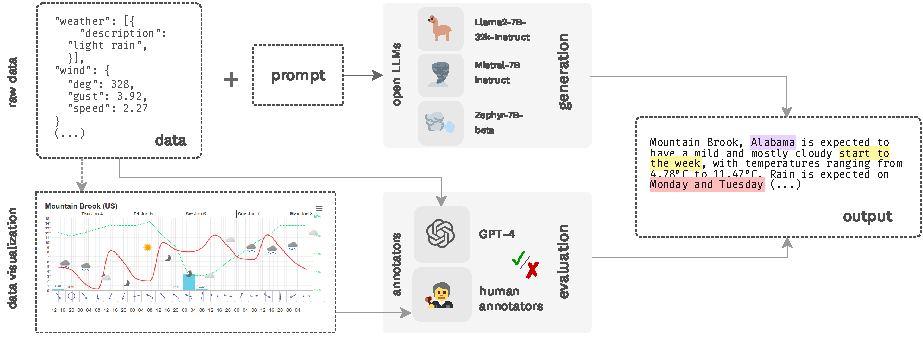
\includegraphics[width=\textwidth]{img/quintd_process.pdf}
%     \caption{Our experimental setup. We first generate the outputs using \acp{llm} that are given raw data and a task-specific prompt. We annotate the token-level semantic errors in the \ac{llm} outputs with (a) an automatic metric based on GPT-4 that matches the output to the raw data, and (b) human annotators, who annotate the errors in the output given the data visualization.}\label{fig:process}
% \end{figure*}

% \paragraph{Models}
% \label{sec:models}
% For our experiments, we selected the following \acp{llm} available under an open license:

% \begin{itemize}
%     \item \textbf{Llama2} \cite{touvron2023llama,llama-2-7b-32k},\\ \texttt{\small together\-computer\-/Llama-2-7B\--32K-Instruct}
%     \item \textbf{Mistral} \cite{jiangMistral7B2023},\\ \texttt{\small mistralai/Mistral-7B-Instruct-v0.1}
%     \item \textbf{Zephyr}  \cite{tunstallZephyrDirectDistillation2023}. \\ \texttt{\small HuggingFaceH4/zephyr-7b-beta}
% \end{itemize}

% The models are instruction-tuned, operate with 32k context, and perform well on recent benchmarks. All the models have 7B parameters and thus fit on a single NVIDIA A40 (48G VRAM) in 16-bit precision.  The models are available through HuggingFace \cite{wolf2019huggingface}.

% We accessed the models via an API provided by the \texttt{text-generation-webui} framework\footnote{\url{https://github.com/oobabooga/text-generation-webui}} running locally.
% For the final experiments, we also included GPT-3.5 (\texttt{gpt-3.5-turbo-1106}) accessed through the OpenAI API \cite{chatgpt}.

% \paragraph{Observations from Preliminary Experiments}
% \label{sec:observations}
% During development, we made several observations which we took into account for our final experimental setup:

% \paragraph{Any input field may appear in the output.} The models do not always select the most relevant fields for the given output. For example, we observed that the models commonly mention identifiers, timestamps, files, and other metadata, leading to unnatural outputs. Due to this, we decided not to include these irrelevant fields in the input.

% \paragraph{Units need to be specified explicitly.} If the units are not specified in the data record, the models tend to resort to their best guess. This may go unnoticed if the unit is evident from the context (e.g., the model will usually not report the temperature in Fahrenheit instead of Celsius), but it may get problematic if the value is ambiguous (e.g., wind speed in km/h versus m/s). Therefore, we explicitly add units to all data records where appropriate.

% \paragraph{Understandable labels are enough.} On the flip side, we decided not to add extra descriptions to the keys if the key was understandable from the label (e.g., \texttt{homeTeam} or \texttt{dimensions}). As discussed by \citet{kasner2023mind}, pretrained models tend to interpret the fields correctly as long as the label is human-readable. We only decided to include chart metadata for the CSV files in the \texttt{owid} domain.

% \paragraph{Long inputs can be troublesome.} The inputs in some domains can easily get longer than 10-20k tokens. This issue is amplified by the fact that the evaluated \acp{llm} tokenize numbers into individual digits. To accommodate for the long inputs, we picked models that accept up to 32k tokens.\footnote{For this reason, we use Llama-2-7B-32k with 32k token context \cite{llama-2-7b-32k} instead of the official Llama-2-7B-Instruct, which only supports 4k context \cite{touvronLlamaOpenFoundation2023}.} However, with long inputs, the GPU memory consumption also gets considerably higher, so we needed to downsample the data in \texttt{owid} and \texttt{openweather} to keep their length under \textasciitilde 8k tokens.


% \paragraph{Few-shot experiments are infeasible.} Due to the context-length limitations described above, we were not able to conduct few-shot experiments since we could not robustly fit an additional ($x_\text{example}$, $y_\text{example}$) pair in the prompt. We attempted to include only $y_\text{example}$ (making the setup ``half-shot''), but we observed that the models then tended to use entities from the example (unrelated to the actual input) in their outputs. Therefore, we decided not to follow this line of experiments (see §\ref{sec:future} for discussion).

% \paragraph{Deterministic decoding and sampling are on par.} In our preliminary experiments, we observed a roughly similar output quality for both deterministic decoding and sampling.\footnote{We used the \texttt{text-generation-webui} default decoding parameters: \texttt{temperature}=0.7, \texttt{top\_p}=0.9, and \texttt{top\_k}=20.} For the final experiments, we decided to use deterministic decoding, which is non-parametric and conceptually more suitable for D2T generation.

% \paragraph{Prefixing the output makes parsing easier.} Even with variations of a \textit{``generate only the output''} instruction appended to the prompt, the models (especially Llama2) tended to first confirm the request. For that reason, we decided to prefix the input for all the models with \textit{``Sure! Here is the \{output\_type\}: "''}. The opening quote at the end of the prefix allowed us to robustly parse the text simply by stripping the closing quote from the model output.

% \paragraph{The outputs are fluent but inaccurate.} We observed that the vast majority of model outputs were grammatically and stylistically correct, capturing the output type specified in the prompt. However, we also noticed that the outputs contained many factual errors (even after emphasizing the focus on factual accuracy in the prompt, see Figure \ref{fig:prompt}). This observation led us to evaluate the model outputs using token-level annotations focused on semantic accuracy errors \cite{reiterSharedTaskEvaluating2020}.



% \paragraph{Final Experiments}
% \label{sec:basic}

% Taking the observations in §\ref{sec:observations} into account, we proceeded to generate the outputs on the test set of \benchmark for token-level error analysis. We first preprocessed the data as mentioned: we stripped out unnecessary fields, added units, and downsampled the data to fit the context. For all the models mentioned in §\ref{sec:models}, we used the prompt in Figure \ref{fig:prompt} and deterministic decoding with a maximum length of 512 tokens.

% For comparison, we also generated outputs for the same inputs and identical prompts with GPT-3.5.\footnote{We did not include GPT-3.5 in our preliminary experiments since closed models are not our focus. We also did not use GPT-4 because we reserve the model for evaluation; see §\ref{sec:gpt4eval}.} Note that even though we fixed the temperature and seed to $0$, the rest of the decoding parameters are inaccessible to us and may differ from the parameters we used for the open models.





% \section{Evaluation}
% \label{sec:eval}
% For evaluation, we focus on \textit{semantic accuracy} errors. We compare the generated texts to the input data, looking for parts of texts that are not faithful to the input data. We annotate the errors on the token level, considering all the tokens in the output text as potential sources of errors.

% Regarding the error taxonomy, we settled on four error categories: \errinc{INCORRECT}, \errnc{NOT\_CHECKABLE}, \errmis{MISLEADING}, and \errother{OTHER}. The taxonomy is inspired by the methodology discussed in \citet{thomsonGoldStandardMethodology2020} and \citet{thomson2023evaluating}. To keep the annotation tractable, we decided not to distinguish between fine-grained categories (e.g., \textit{incorrect name} vs. \textit{incorrect number}). The descriptions of our error categories, as presented in the instructions for annotation, are included in Table \ref{tab:errors}.

% \begin{table*}[t]
%     \small
%     \centering
%     \begin{tabular}{p{2.25cm}p{12.5cm}} \toprule                                                                                        \\
%         \textbf{Error}         & \textbf{Description}                                                                        \\ \midrule
%         \errinc{INCORRECT}     & The fact in the text contradicts the data.                                                  \\
%         \errnc{NOT\_CHECKABLE} & The fact in the text cannot be checked given the data.                                      \\
%         \errmis{MISLEADING}    & The fact in the text is misleading in the given context.                                    \\
%         \errother{OTHER}       & The text is problematic for another reason, e.g., grammatically or stylistically incorrect,
%         irrelevant, or repetitive.                                                                                           \\\midrule

%         \textbf{Example}       &                                                                                             \\

%         \textit{data}          &
%         \textbf{Nokia 3310} |
%         \textit{color}: black, blue, grey |
%         \textit{display}: 320x240px                                                                                          \\
%         \textit{text}          &
%         Nokia 3310 is \errnc{produced in Finland} and features a \errinc{320x320} display. It is \errmis{misleading}{available in black color}. \errmis{other}{The data seem to provide only partial information about the phone.}
%         \vspace*{0.1cm}
%         \\ \bottomrule
%         % \textit{explanation}                             &
%         % \begin{description}[nosep]\item[produced in Finland] The country where the phone is produced is not mentioned in the data.
%         %   \item[320x320] The data mentions that the display has resolution 320x240px.
%         %   \item[available in black color] Misleadingly suggests that the phone is not available in other colors.
%         %   \item[The data seem to provide (...)] The note is irrelevant for the phone description.      \end{description}                                                                                                                                                                                                                                   \\\bottomrule
%     \end{tabular}
%     \caption{Categories of errors annotated in our evaluation and an example demonstrating the error types. See Appendix \ref{app:humeval} for an explanation of individual errors in the example.}
%     \label{tab:errors}
% \end{table*}

% We employ two complementary evaluation schemes:
% \begin{itemize}
%     \item \gptmetric{}: \textbf{an automatic metric} based on GPT-4 (§\ref{sec:gpt4eval}),
%     \item \humanmetric{}: \textbf{human evaluation} based on crowdsourcing (§\ref{sec:humaneval}).
% \end{itemize}

% These two schemes are based on similar instructions and produce (nearly) equivalent outputs. The main idea in introducing multiple schemes is to compensate for the shortcomings of each approach and thus increase the replicability and robustness of our results.


% \paragraph{GPT-4-based Evaluation}
% \label{sec:gpt4eval}

% \ac{llm}-based metrics can be customized for a particular task without the need for training data. For our experiments, we employ a metric based on GPT-4 (\texttt{gpt-4-1106-preview}, \citealp{openai2023gpt4}), which was shown to be superior in following fine-grained instructions compared to other \acp{llm} and to have high correlations with human judgment on evaluating generated texts  \cite{zhaoInvestigatingTabletoTextGeneration2023,sottanaEvaluationMetricsEra2023,kocmiGEMBAMQMDetectingTranslation2023,kocmiLargeLanguageModels2023}.
% % Compared to using fine-tuned models for token-level evaluation \cite{kasnerTextinContextTokenLevelError2021}, this allows us to customize the metric for a particular task without the need for training data.

% \gptmetric{} is instantiated using a prompt and a system message describing the task. We instruct the model to produce a JSON output with sequentially ordered errors using the following format:

% \small
% \begin{verbatim}
% {
%   "errors": [{
%     "reason": [REASON],
%     "text": [TEXT_SPAN],
%     "type": [ERROR_CATEGORY]
%     }, 
%     ...]
% }.
% \end{verbatim}
% \normalsize


% Note that we require that the model first generates the free-form text \textit{reason} for the error. Generating the reason incurs almost no extra cost, and our cursory observations suggest that requiring it leads to more precise outputs.

% Concerning the alignment of the model outputs with the original text, we perform matching on \texttt{TEXT\_SPAN}. We ensure that the model response is a valid JSON using OpenAI's \texttt{response\_format} parameter.  See Appendix \ref{app:gpt4eval} for more details about the metric, including the prompt and the system message.


% \paragraph{Human-based Evaluation}
% \label{sec:humaneval}

% An automatic metric based on a closed \ac{llm} makes the evaluation potentially non-reproducible and biased \cite{kocmiGEMBAMQMDetectingTranslation2023,wangLargeLanguageModels2023}, for which we compensate by obtaining annotations from human annotators.

% For the human annotation metric \humanmetric{}, we prepared a custom web interface
% %  based
% %%% TODO %%% 
% % \OD{remove cite for anonymized version?}
% %%% %%% 
% % on \textsc{TabGenie} \cite{kasner2023tabgenie}, 
% where an annotator is able to annotate a text span with a selected error category. We created custom visualizations for each data format. Unlike with \gptmetric{}, we did not ask the crowdworkers for free-form reasoning about the errors since that would make the annotation more complex.

% We hired annotators on the Prolific crowdsourcing platform.\footnote{\url{https://prolific.com}} In total, we hired 100 annotators, each annotating 20 examples (4 model outputs for each of the five domains). We selected annotators with at least 10 completed tasks and a 100\% approval rate, having English as their primary language. We paid the annotators \textsterling 9 per hour, according to the platform's recommendations. The median time for completing the annotations was 47 minutes. See Appendix \ref{app:humeval} for the instructions for the annotators and the annotation interface and Appendix \ref{app:outputs} for the data visualizations.




% % \paragraph{Evaluating Controllability}

% % Due to our resource limitations, we were not able to run the token-level error annotations for all the stylized outputs. Instead, we randomly selected 10 outputs for each domain on which we run the GPT-4 annotations, and two annotators (authors of the paper) rated the adherence to style along with free-form comments.

% \section{Results and Discussion}
% \label{sec:discussion}

% A summary of the token-level annotations is in Table \ref{tab:results_agg} and \ref{tab:results_errperex}, with detailed results per domain provided in Appendix \ref{app:full_results}.


% \begin{table*}[ht]
%     \small
%     \centering
%     \begin{tabular}{lccccccccccr}
%         \toprule
%                          & \multicolumn{2}{c}{\textbf{Incorrect}} & \multicolumn{2}{c}{\textbf{Not Checkable}} & \multicolumn{2}{c}{\textbf{Misleading}} & \multicolumn{2}{c}{\textbf{Other}} & \multicolumn{2}{c}{\textbf{All categories}} &                                                                                                     \\
%                          & \gptmetric{}                           & \humanmetric{}                             & \gptmetric{}                            & \humanmetric{}                     & \gptmetric{}                                & \humanmetric{} & \gptmetric{}  & \humanmetric{} & \gptmetric{}  & \humanmetric{} & \# \textbf{Tok.} \\\midrule

%         \textbf{Llama2}  & \textbf{2.46}                          & 1.57                                       & 0.90                                    & 1.25                               & \textbf{0.20}                               & 0.25           & 0.13          & \textbf{0.10}  & 3.70          & 3.18           & 83.8             \\
%         \textbf{Mistral} & 2.80                                   & 2.03                                       & 0.52                                    & 1.12                               & 0.37                                        & 0.44           & 0.11          & 0.25           & 3.80          & 3.85           & 114.9            \\
%         \textbf{Zephyr}  & 2.50                                   & \textbf{1.44}                              & \textbf{0.40}                           & \textbf{0.77}                      & 0.39                                        & \textbf{0.20}  & \textbf{0.06} & 0.16           & \textbf{3.35} & \textbf{2.58}  & 98.0             \\ \cdashlinelr{1-12}
%         \textbf{GPT-3.5} & 1.57                                   & 0.65                                       & 0.32                                    & 0.49                               & 0.42                                        & 0.18           & 0.02          & 0.07           & 2.32          & 1.39           & 84.9             \\ \bottomrule
%     \end{tabular}
%     \caption{The average \textit{numbers of errors per output} (lower is better) based on GPT-4 (\gptmetric{}) and human annotators (\humanmetric{}). We also include the average number of tokens per output in the rightmost column. The results of the best open \ac{llm}  are emphasized.}
%     \label{tab:results_agg}
% \end{table*}


% \begin{table*}[ht]
%     \small
%     \centering
%     \begin{tabular}{lcccccccccc}
%         \toprule
%                          & \multicolumn{2}{c}{\textbf{Incorrect}} & \multicolumn{2}{c}{\textbf{Not Checkable}} & \multicolumn{2}{c}{\textbf{Misleading}} & \multicolumn{2}{c}{\textbf{Other}} & \multicolumn{2}{c}{\textbf{All categories}}                                                                                    \\
%                          & \gptmetric{}                           & \humanmetric{}                             & \gptmetric{}                            & \humanmetric{}                     & \gptmetric{}                                & \humanmetric{} & \gptmetric{}  & \humanmetric{} & \gptmetric{}  & \humanmetric{} \\\midrule
%         \textbf{Llama2}  & 0.78                                   & 0.53                                       & 0.46                                    & 0.57                               & \textbf{0.15}                               & 0.17           & 0.09          & \textbf{0.08}  & 0.92          & 0.86           \\
%         \textbf{Mistral} & 0.78                                   & 0.54                                       & 0.32                                    & 0.50                               & 0.23                                        & 0.21           & 0.08          & 0.14           & 0.93          & 0.81           \\
%         \textbf{Zephyr}  & \textbf{0.77}                          & \textbf{0.47}                              & \textbf{0.26}                           & \textbf{0.42}                      & 0.27                                        & \textbf{0.16}  & \textbf{0.04} & 0.12           & \textbf{0.88} & \textbf{0.76}  \\\cdashlinelr{1-11}
%         \textbf{GPT-3.5} & 0.64                                   & 0.38                                       & 0.21                                    & 0.29                               & 0.26                                        & 0.13           & 0.02          & 0.06           & 0.75          & 0.61           \\ \bottomrule
%     \end{tabular}
%     \caption{The ratio of \textit{outputs containing at least one error} (lower is better) based on GPT-4 (\gptmetric{}) and human annotators (\humanmetric{}). The results of the best open \ac{llm}  are emphasized.}
%     \label{tab:results_errperex}
% \end{table*}



% \paragraph{How Accurate Are the Model Outputs?}
% Depending on the model, between 74-85\% of examples contain an error according to \humanmetric, suggesting that open \acp{llm} make semantic errors very often. According to \gptmetric, the number is as high as 88-93\%.

% The most common error type is \texttt{INCORRECT}. As shown in Table \ref{tab:results_agg}, all the open \acp{llm} make more than \textbf{two statements contradicting the data per output on average}. The \texttt{NOT\_CHECKABLE} errors are also relatively common: more than one per output on average according to \humanmetric, and at least one being present in more than 26\% of examples according to both metrics.

% The results vary widely according to the domain (see Appendix \ref{app:full_results}). For example, the outputs in \texttt{wikidata} contain much more \texttt{NOT\_CHECKABLE} errors on average (1.54 per output according to \humanmetric) than  \texttt{INCORRECT} errors (0.12 per output according to \humanmetric), suggesting that with simpler inputs, the models tend to introduce extra information. The \texttt{openweather} domain seems to be the most complex with the longest outputs (\textasciitilde 164 tokens), more than eight errors in the output on average, and >90\% of outputs containing an error.

% The differences between the open \acp{llm} are not major. Out of the open \acp{llm}, Zephyr has the best results across categories and metrics, followed by Llama2. However, the outputs of Mistral are longer on average, leaving more space for errors. GPT-3.5 (which we consider separately) does generally better according to both \gptmetric and \humanmetric, although it still makes an error in 60-75\% of examples (2 errors per example on average). In general, the results show that \acp{llm} make too many semantic errors to be usable in practice for D2T generation in a zero-shot setting.



% \paragraph{Do Evaluation Methods Agree?}
% \label{sec:metricscorr}
% To quantify the agreement of our evaluation metrics, we computed the Pearson correlation coefficient between the error counts on the level of tokens, examples, and domains (see Appendix \ref{app:corr} for details). The correlation on the level of tokens is weak ($r_{\text{token}}=0.26$) but gets better on the example-level ($r_{\text{example}}=0.55$) and even better on the domain-level ($r_{\text{domain}}=0.92$). In Table \ref{tab:errors_tokenlevel}, we show the percentage of tokens marked by individual metrics. The metrics agree on the specific tokens in less than 6\%, although they both mark around 21\% of tokens as erroneous.
% % , suggesting that the error spans may be subject to interpretation.

% We also measure inter-annotator agreement between human annotators. For that, we obtained annotations from two annotators for 100 model outputs. The results are similar: the annotators agree weakly on the token level ($r_{\text{token}}=0.36$), stronger on the example level ($r_{\text{example}}=0.53$), and even stronger on the domain level ($r_{\text{domain}}=0.85$). We conclude that while the details regarding error spans and categories may vary, the annotators as well as GPT-4 generally agree on the accuracy of model outputs for a given set of examples. In the future, the agreement could be improved by measuring errors on the phrase level \cite{vamvas2022little}.

% % The results show that while \gptmetric and \humanmetric do not agree much on individual token spans, they correlate well for high-level ranking of the models.

% \begin{table}[t]
%     \small
%     \centering
%     \begin{tabular}{lccc}
%         \toprule
%         {}                       & \gptmetric{} & \humanmetric{} & \gptmetric{} + \humanmetric{} \\
%         \midrule
%         \bfseries Incorrect      & 0.135        & 0.099          & 0.040                         \\
%         \bfseries Not checkable  & 0.039        & 0.076          & 0.016                         \\
%         \bfseries Misleading     & 0.022        & 0.022          & 0.001                         \\
%         \bfseries Other          & 0.008        & 0.018          & 0.001                         \\
%         \bfseries All categories & 0.204        & 0.214          & 0.059                         \\
%         \bottomrule
%     \end{tabular}
%     \caption{The ratio of \textit{tokens marked as erroneous} by GPT-4 (\gptmetric), human annotators (\humanmetric), and both metrics at the same time (\gptmetric + \humanmetric).}
%     \label{tab:errors_tokenlevel}
% \end{table}


% % \begin{table}[t]
% %   \small
% %   \centering
% %   \begin{tabular}{lrrrr}
% %     \toprule
% %                & \gptmetric{} & \humanmetric{} & \textbf{Both} & \textbf{None} \\
% %     \midrule
% %     Total (\%) & 11.68        & 12.72          & 5.88          & 66.89         \\    \bottomrule
% %   \end{tabular}
% %   \caption{Percentage of tokens annotated with an error (of any category) by GPT-4 (only), human annotators (only), both metrics at the same time, or none of the metrics.}
% % \end{table}


% \paragraph{Recommendations and Directions}
% \label{sec:future}
% \paragraph{Forget fluency, solve accuracy.} The output of \acp{llm} is satisfactory regarding the style, format, and purpose of the text. However, the amount of semantic errors remains very high. Improving the semantic accuracy of the models
% %%% TODO %%%
% % \OD{remove Pat's cite for anonymization} \cite{schmidtova2023semantic}
% %%% %%%
% \cite{li2022faithfulness}, along with new model-based evaluation metrics \cite{liuGEvalNLGEvaluation2023,xuINSTRUCTSCOREExplainableText2023}, could thus help to bring improve \ac{llm}-based D2T generation systems where it is most needed.



% \paragraph{Use efficient models.} The memory issues with long context, making few-shot experiments infeasible, can potentially be solved by using more efficient long-context models equipped with Flash Attention \cite{dao2022flashattention} and fast inference libraries such as \texttt{llama.cpp}.\footnote{\url{https://github.com/ggerganov/llama.cpp}} A potentially suitable open \ac{llm} in this respect is the long-context Llama2 (\citealp{xiong2023effective}; model to be released).


% \paragraph{Test the models in the wild.} Except for using an ad-hoc dataset of real-world data as we did in our work, the ecological validity of D2T evaluation can also be ensured by continuous evaluation with human users \cite{zheng2023judging} and evaluating the real-world impact of the systems \cite{reiter2023impact}.


% \paragraph{Multilinguality is an opportunity.}With the recent efforts in extending D2T generation to low-resource languages \cite{cripwell-etal-2023-2023}, multilingual D2T generation with open \acp{llm} seems a promising direction. Although we did not go beyond English, initial steps were already done by works such as \citet{lorandi2023data}.


% \paragraph{Be careful about subtle bugs.} During our preliminary experiments, we uncovered subtle bugs in API calls such as incorrect instruction templates\footnote{\url{https://huggingface.co/docs/transformers/chat_templating}} or involuntary input truncation. With the apparent ease of API access and robustness of \acp{llm}, such bugs could go unnoticed and artificially skew the model performance.






\chapter{Conclusions}
\label{chap:conclusions}

In this thesis, we set out to explore how to efficiently employ neural \acp{lm} in \ac{d2t} generation systems 
to improve their fluency and flexibility. 
Although the capabilities of \acp{lm} have increased rapidly, the issues that we were trying to solve---semantic inaccuracies in the generated texts, lack of automatic evaluation metrics, heterogeneous input data format, and unknown scope of \acp{lm} abilities---are still pressing. That is not to say that there has not been any progress on these topic, quite the opposite. We listed numerous research works which pushed the progress in these topics forward in \autoref{chap:background}.


Hopefully, we also contributed to the progress with our findings, including:
\begin{itemize}
    \item Our approaches for efficient employment of \acp{plm} in \ac{d2t} generation systems by constraining their role to improving text fluency (\autoref{chap:low-res}),
    \item Our automatic metrics for evaluating semantic accuracy of generated texts based on \acp{plm} (\autoref{chap:evaluation}),
    \item Our toolkit for unified processing and visualization of existing benchmarks (\autoref{chap:tabgenie}),
    \item Our analyses of generalization abilities of \acp{plm} to new data labels and \acp{llm} to common data formats.
\end{itemize}

As neural \acp{lm} proliferate in \ac{nlp}, we can now safely say that systems based on neural models are here to stay. Our best bet is therefore to devise ways to safely employ them in the existing systems. \ac{d2t} generation is a specific area that goes contrary to what \acp{lm} offer.


%
% TEXT END
%

\renewcommand{\chapterheadstartvskip}{\vspace*{0mm}} % chapter spacing

\cleardoublepage{}
\bibliographystyle{csplainnat}
\addcontentsline{toc}{chapter}{Bibliography}
{\small \bibliography{references}}

\cleardoublepage{}
\addcontentsline{toc}{chapter}{List of Abbreviations}
\renewcommand*{\acronymname}{List of Abbreviations}
\printglossary[type=\acronymtype,style=index]

\addcontentsline{toc}{chapter}{List of Tables}
{\small \listoftables\par}

\addcontentsline{toc}{chapter}{List of Figures}
{\small \listoffigures\par}

\cleardoublepage{}
\addcontentsline{toc}{chapter}{List of Publications}
\chapter*{List of Publications}

\phantom{\nobibliography*{references}}

% -----------------------------------------------------------------------------

\noindent\bibentry{kasnerTrainHardFinetune2020}
\begin{itemize}[noitemsep,topsep=0pt]

    \item The data-to-text generation system based on the finetuned mBART model (\autoref{sec:finetuning}).
    \item Our submission for the WebNLG+ shared task.
    \item Citations (without self-citations): 9
\end{itemize}\vspace{.5\baselineskip}

% -----------------------------------------------------------------------------
\noindent\bibentry{kasnerDatatoTextGenerationIterative2020}
\begin{itemize}[noitemsep,topsep=0pt]
    \item The data-to-text generation system based on iterative text editing (\autoref{sec:iterative}).
    \item Citations (without self-citations): 17

\end{itemize}\vspace{.5\baselineskip}

% -----------------------------------------------------------------------------
\noindent\bibentry{kasner2022neural}
\begin{itemize}[noitemsep,topsep=0pt]
    \item The data-to-text generation system based on a pipeline of neural modules (\autoref{sec:pipeline}).
    \item Citations (without self-citations): 21

\end{itemize}\vspace{.5\baselineskip}

% -----------------------------------------------------------------------------
\noindent\bibentry{dusekEvaluatingSemanticAccuracy2020}
\begin{itemize}[noitemsep,topsep=0pt]

    \item The metric for detecting omissions and hallucinations in generated texts (\autoref{sec:tok-eval}).
    \item Best short paper at INLG 2020.
    \item Citations (without self-citations): 47

\end{itemize}\vspace{.5\baselineskip}


% -----------------------------------------------------------------------------
\noindent\bibentry{kasnerTextinContextTokenLevelError2021}
\begin{itemize}[noitemsep,topsep=0pt]
    \item The metric for token-level error detection in generated texts (\autoref{sec:tok-eval})
    \item Our submission to the shared task Evaluating Accuracy in Generated Texts.
    \item Citations (without self-citations): 6

\end{itemize}\vspace{.5\baselineskip}


% -----------------------------------------------------------------------------
\noindent\bibentry{kasnerTabGenieToolkitTabletoText2023}
\begin{itemize}[noitemsep,topsep=0pt]

    \item The toolkit for processing and visualization of data-to-text generation datasets (\autoref{sec:tabgenie}).
    \item Citations (without self-citations): 2

\end{itemize}\vspace{.5\baselineskip}


% -----------------------------------------------------------------------------
\noindent\bibentry{kasnerMindLabelsDescribing2022}
\begin{itemize}[noitemsep,topsep=0pt]

    \item The analysis of verbalizing relations in knowledge graphs with pretrained language models (\autoref{sec:rel2text}).
    \item Citations (without self-citations): 3

\end{itemize}\vspace{.5\baselineskip}


% -----------------------------------------------------------------------------
\noindent\bibentry{kasnerReferenceBasedMetricsAnalyzing2024}
\begin{itemize}[noitemsep,topsep=0pt]

    \item The analysis of data-to-text generation with open large language models (\autoref{sec:quintd}).
    \item Citations (without self-citations): 2

\end{itemize}\vspace{.5\baselineskip}

\vfill

\noindent Only publications relevant to this thesis are included. The number of
citations was computed using Semantic Scholar API. Total number of citations of
publications related to the topic of the thesis (without self-citations) by June 14, 2024: {\bf 107}.


\end{document}
